\def \title{An SDR-based FRS Transceiver}
\def \subtitle{Prototyping a Multi-channel FRS Transceiver with CTCSS Support via GNU Radio and the Nuand bladeRF}

\def \authors{
  \begin{table}[h]
    \centering
    \begin{tabular}{ccc}
      Robert Ghilduta & Brian Padalino & Jon Szymaniak \\
      \href{mailto:robert.ghilduta@nuand.com?cc=bladeRF@nuand.com}{robert.ghilduta@nuand.com} & \href{mailto:bpadalino@nuand.com?cc=bladeRF@nuand.com}{bpadalino@nuand.com} & \href{mailto:jon@nuand.com?cc=bladeRF@nuand.com}{jon@nuand.com}
    \end{tabular}
  \end{table}
  ~\\
}

\def \tablerowcolor{\rowcolor[HTML]{C0C0C0}}
\def \tablecolcolor{\columncolor[HTML]{C0C0C0}}

\def \revisions {
  \begin{table}[h]
    \centering
    \begin{tabular}{|c|c|l|}
      \hline
      \tablerowcolor
      \textbf{Revision} & Date & \textbf{Summary} \hspace{4in}  \\ \hline
      1  & 2015-06-12 & Initial public draft \\ \hline
    \end{tabular}
  \end{table}
}

%-------------------------------------------------------------------------------
%
% This template is a modified version of what is provided at:
%    https://github.com/lungetech/proposal-template
% 
% Copyright (c) 2015, Nuand, LLC
% Copyright (c) 2013, Lunge Technology, LLC
% All rights reserved.
% 
% Redistribution and use in source and binary forms, with or without modification,
% are permitted provided that the following conditions are met:
% 
%   Redistributions of source code must retain the above copyright notice, this
%   list of conditions and the following disclaimer.
% 
%   Redistributions in binary form must reproduce the above copyright notice, this
%   list of conditions and the following disclaimer in the documentation and/or
%   other materials provided with the distribution.
% 
%   Neither the name of the Lunge Technology, LLC nor the names of its
%   contributors may be used to endorse or promote products derived from
%   this software without specific prior written permission.
% 
% THIS SOFTWARE IS PROVIDED BY THE COPYRIGHT HOLDERS AND CONTRIBUTORS "AS IS" AND
% ANY EXPRESS OR IMPLIED WARRANTIES, INCLUDING, BUT NOT LIMITED TO, THE IMPLIED
% WARRANTIES OF MERCHANTABILITY AND FITNESS FOR A PARTICULAR PURPOSE ARE
% DISCLAIMED. IN NO EVENT SHALL THE COPYRIGHT HOLDER OR CONTRIBUTORS BE LIABLE FOR
% ANY DIRECT, INDIRECT, INCIDENTAL, SPECIAL, EXEMPLARY, OR CONSEQUENTIAL DAMAGES
% (INCLUDING, BUT NOT LIMITED TO, PROCUREMENT OF SUBSTITUTE GOODS OR SERVICES;
% LOSS OF USE, DATA, OR PROFITS; OR BUSINESS INTERRUPTION) HOWEVER CAUSED AND ON
% ANY THEORY OF LIABILITY, WHETHER IN CONTRACT, STRICT LIABILITY, OR TORT
% (INCLUDING NEGLIGENCE OR OTHERWISE) ARISING IN ANY WAY OUT OF THE USE OF THIS
% SOFTWARE, EVEN IF ADVISED OF THE POSSIBILITY OF SUCH DAMAGE.
%
%-------------------------------------------------------------------------------

\documentclass[letterpaper,12pt]{article}

\usepackage[printonlyused]{acronym}
\usepackage{amsmath}
%\usepackage[font={small,sf},labelfont={small,sf}]{caption}
\usepackage{float}
\usepackage{caption}
\usepackage{color}
\usepackage{fancyhdr}
\usepackage[includeheadfoot,left=1in,top=.4in,right=1in,bottom=.75in,headsep=\dimexpr3cm-59pt\relax,headheight=59pt]{geometry}
\usepackage{graphicx}
%\usepackage[pagebackref,hyperindex=true]{hyperref}
\usepackage[hidelinks]{hyperref}
\usepackage{listings}
\usepackage{longtable}
\usepackage{mdwlist}
\usepackage{parskip}
\usepackage{setspace}
\usepackage{tabularx}
\usepackage[compact]{titlesec}
\usepackage{xfrac}
\usepackage{xspace}
\usepackage[table,xcdraw]{xcolor}

% default font packages
\usepackage{courier} % use courier for the mono-spaced font 
\usepackage{helvet}  % use a Helvetica clone for default text (sans-serif)

% Uses PDF page rotate attr. Change to lscape if PDF output is not desired.
\usepackage{pdflscape}  

% Drawings
\usepackage[siunitx, american, smartlabels, cute inductors, europeanvoltages]{circuitikz}

%%%
% default document settings
%%%

% setup the default fonts for section headers
\titleformat*{\section}{\sffamily\fontsize{16}{16}\selectfont\bfseries}
\titleformat*{\subsection}{\sffamily\fontsize{14}{14}\selectfont\bfseries}
\titleformat*{\subsubsection}{\sffamily\fontsize{12}{12}\selectfont\bfseries}
\titleformat*{\paragraph}{\sffamily\fontsize{12}{12}\selectfont\bfseries}
\titleformat*{\subparagraph}{\sffamily\fontsize{12}{12}\selectfont\bfseries}

% section numbering
\setcounter{tocdepth}{3}     % display only 3 sections deep in the table of contents
\setcounter{secnumdepth}{5}  % number to 5 sections deep

% add acronyms to the TOC (use chapter, if chapters are available, otherwise use sections
% Based off of suggestions at: http://jevopi.blogspot.com/2009/09/acronyms-and-latex.html
\providecommand{\listofacronymsname}{List of Acronyms and Abbreviations}
\providecommand{\listofacronyms}{
    \ifx\chapter\undefined
        \chapter*{\listofacronymsname}
	    % \addcontentsline{toc}{chapter}{\listofacronymsname}
    \else
        \section*{\listofacronymsname}
		% \addcontentsline{toc}{section}{\listofacronymsname}
    \fi
    \label{sec:acronyms}
	\markboth{\listofacronymsname}{\listofacronymsname}
    \begin{acronym}[AAAAAAAAAAA]
\acro{CPFSK}{Continuous-Phase Frequency Shift Keying}
\acro{CPU}{Central Processing Unit}
\acro{CTCSS}{Continuous Tone-Coded Squelch System}
\acro{CVSD}{Continuously Variable Slope Delta}
\acro{DAC}{Digital to Analog Converter}
\acro{FIR}{Finite Impulse Response}
\acro{FPGA}{Field Programmable Gate Array}
\acro{FRS}{Family Radio Service}
\acro{HDL}{Hardware Description Language}
\acro{IIR}{Infinite Impulse Response}
\acro{GMRS}{General Mobile Radio Service}
\acro{GRC}{GNU Radio Companion}
\acro{GUI}{Graphical User Interface}
\acro{LNA}{Low Noise Amplifier}
\acro{LPF}{Low Pass Filter}
\acro{NBFM}{Narrow-Band Frequency Modulation}
\acro{PLL}{Phase Locked Loop}
\acro{RF}{Radio Frequency}
\acro{RX}{Receive}
\acro{SIB}{Service Indicator Bit}
\acro{SINAD}{Signal-to-Noise and Distoration ratio}
\acro{SDR}{Software Defined Radio}
\acro{TX}{Transmit}
\acro{VCO}{Voltage Controlled Oscillator}
\acro{VGA}{Variable Gain Amplifier}
\acro{VSA}{Vector Signal Analyzer}
\acro{VSG}{Vector Signal Generator}
\end{acronym}

}

%%%
% custom page styles
%%%

\fancypagestyle{plain}{
    \ifdefined\headerleft
      \fancyhead[L]{\headerleft}
    \else
      \fancyhead[L]{}
    \fi
    \ifdefined\headercenter
      \fancyhead[C]{ \textbf{\headercenter}}
    \else
      \fancyhead[C]{ \textbf{\title}}
    \fi
    \fancyhead[R]{ Nuand, LLC}
    \fancyfoot[L]{}
    \fancyfoot[C]{}
    \fancyfoot[R]{\small \thepage}
}

% set the default page style to "plain"
\pagestyle{plain}

%%%
% page templates
%%%

\newcommand{\whitepapercover}{
    \begin{titlepage}
    \thispagestyle{empty}
    \vspace*{1.25in}

    \hfill \textsc{\sffamily\huge\bfseries \MakeLowercase{\title}} \\
    \begin{flushright}
      \ifdefined\subtitle
      \textsc{\sffamily\large \MakeLowercase{\subtitle}} \\
      \vspace*{0.25in}
      \fi
      \textsc{\sffamily\large \MakeLowercase{\today}}
    \end{flushright}

    \vspace{2.5in}
    \begin{center}
        
\includegraphics[width=4.0in]{images/logo.png}
    \end{center}

    \end{titlepage}
    \cleardoublepage
}

\newcommand{\bib}{
    \cleardoublepage
    \pagestyle{plain}
    \phantomsection
    \ifx\chapter\undefined
        \addcontentsline{toc}{chapter}{References}
    \else
        \addcontentsline{toc}{section}{References}
    \fi
    \bibliographystyle{unsrt} % unsrt = plain, except sorted by use, not date.
    {
        \raggedright
        \bibliography{include/refs}
    }
}

\newcommand{\docinfo}{
    \pagenumbering{roman}
    \thispagestyle{plain}
    \section*{License}
    This work by Nuand, LLC is licensed under:
    \begin{center}
      \footnotesize
      \href{http://creativecommons.org/licenses/by/4.0/}{\texttt{Creative Commons Attribution 4.0 International License}} \\
      \vspace{0.125in}
      \href{http://creativecommons.org/licenses/by/4.0/}{
\includegraphics[width=1in]{images/by.png}}
    \end{center}


    \section*{Authors}
    \authors

    \ifdefined\contributors
        \section*{Contributing Authors}
        \contributors
    \fi

    \newpage
    \section*{Revisions}

    Comments, feedback, improvements, and fixes may be sent to \href{mailto:bladeRF@nuand.com}{\textless{bladeRF@nuand.com}\textgreater}.

    \revisions

    \cleardoublepage

    \tableofcontents

    \cleardoublepage

    \ifdefined \enablefiguretableindex
      \listoftables
      \listoffigures
      \cleardoublepage
    \fi

    \ifdefined \enableacronymlist
      \listofacronyms
      \cleardoublepage
    \fi

    \pagenumbering{arabic}
}

%%%
% ease of use macros
%%%

% Example: \q{foo} 
% Results: "foo" - except the quote marks go the right way.
\newenvironment{q}[1]{``#1''} 

% example: C:$\bs$Program Files$\bs$Adobe$\bs$
% Results: C:\Program Files\Adobe\
\def \bs{\char`\\}

% example: \begin{fig}{figure label}{figure caption}{ ... }
% results: A figure, boxed in the center, with font slightly shrunk, with a label and caption
\newcommand{\temporarylabel}{}
\newcommand{\temporarycaption}{}
\newenvironment{fig}[2]{
    \renewcommand{\temporarylabel}{#1}
    \renewcommand{\temporarycaption}{#2}
    \begin{figure}[!htbp]
    \begin{center}
    \begin{small}
}{
    \end{small}
    \end{center}
    \caption{\temporarycaption \label{\temporarylabel}}
    \end{figure}
}

%%%
% Names of products and tool
%
% Use these to ensure capitalization, trademarks, etc., are consistent
% throughout documents.
%%%
\def \tm{\textsuperscript{\textregistered\:}}
\def \windows{Windows\tm}
\def \matlab{MATLAB\tm}
\def \simulink{Simulink\tm}
\def \fx3{FX3\tm}

%%%
% Macros for various conventions
%%%

% Filename
\newcommand{\fname}[1]{\texttt{#1}}
\newcommand{\program}[1]{\texttt{#1}}

%%%
% Styles for code listings
%%%

\definecolor{code-background}{gray}{0.90}
\definecolor{code-comment}{HTML}{005200}

\lstdefinestyle{cmdline}{
    backgroundcolor=\color{code-background},
    frame=single,
    basicstyle=\scriptsize\ttfamily,
    numberstyle=\tiny,
    numbers=left,
    captionpos=b,
    commentstyle=\itshape\color{code-comment},
    keepspaces=true,
    morecomment=[l]{\#},
}


\begin{document}

\whitepapercover
\docinfo

\section{Intended Audience}
The intended audience for this document is someone with a basic understanding
of frequency domain analysis, sampling theory, digital filtering, and analog
modulation techniques. Prior experience with GNU Radio, \ac{GRC}, \ac{SDR}, and
MATLAB is also beneficial. This paper is likely to be useful for SDR users
looking for examples of:
\begin{itemize}
    \item Narrow-band FM transmitters and receivers
    \item Filter design using software tools
    \item Usage of GNU Radio's polyphase channelizer and synthesizer blocks
    \item Full-duplex operation of the bladeRF
\end{itemize}

\vspace{0.25in}

\section{Abstract}

The Nuand bladeRF is a USB 3.0 \ac{SDR} featuring full-duplex
operation and configurable filter bandwidths that can cover up to 28 MHz.
These properties are leveraged to design and implement a real-time \ac{FRS}
transceiver capable of simultaneously transmitting and/or receiving on any
subset of its 14 channels, with optional \ac{CTCSS} support. The open source
GNU Radio framework and the \ac{GRC} tool are used to realize the transceiver
design as a graphical flowgraph and to create an interactive GUI interface for
the transceiver. This paper presents both a high-level description of the
design, as well as a detailed discussion of the GNU Radio blocks utilized and
the rationale for their associated parameter values. In doing so,
considerations for targeting the bladeRF and accounting for real-world
nonidealties are included. Lastly, the approaches for testing and evaluation
the design using RF test equipment and FRS handhelds is presented, along with
results.

\cleardoublepage

\section{Overview of the Family Radio Service}

\ac{FRS} is a private, 14-channel, two-way data communications service
intended for short-distance voice and data communications \cite{FCC_FRS}. Rules
governing this service are defined in Title 47, Part 95B \cite{FCC_PART_95B}.

The frequency allocations for each of the 14 channels are listed below. Each
channel is allocated 12.5 kHz of bandwidth, and the max deviation of the
narrow band FM signals used on these channels is 2.5kHz \cite{FCC_PART_95B}.

\begin{table}[h]
  \centering
  \caption{FRS frequency allocations}
  \footnotesize
  \begin{tabular}{|c|c||c|c|}
    \hline
    \textbf{Channel}    & \textbf{Frequency (MHz)} &
    \textbf{Channel}    & \textbf{Frequency (MHz)} \\ \hline
    1 & 462.5625 & 8    & 467.5625 \\ \hline
    2 & 462.5875 & 9    & 467.5875 \\ \hline
    3 & 462.6125 & 10   & 467.6125 \\ \hline
    4 & 462.6375 & 11   & 467.6375 \\ \hline
    5 & 462.6625 & 12   & 467.6624 \\ \hline
    6 & 462.6875 & 13   & 467.6875 \\ \hline
    7 & 462.7125 & 14   & 467.7125 \\ \hline
  \end{tabular}
\end{table}

Many handheld \ac{FRS} radios include \ac{CTCSS} support\footnote{CTCSS support
is often marketed as ``sub-codes'' or ``privacy codes.''}, in which receivers
require the presence of a sub-audible tone in order to break squelch. Table
\ref{tab:ctcss}  presents commonly used frequencies for these sub-audible tones.
Note that these CTCSS tones are not part of the FRS standard, but an
industry-created and adopted method for co-channel use between multiple
parties.

\begin{table}[h]
  \centering
  \caption{Common CTCSS tone frequencies, in Hz} \label{tab:ctcss}
  \footnotesize
  \begin{tabular}{|c|c|c|c|c|c|c|c|}
    \hline
    67.0  & 71.9  & 74.4  & 77.0  & 79.7  &  82.5 &  85.4 & 88.5  \\ \hline
    91.5  & 94.8  & 97.4  & 100.0 & 103.5 & 107.2 & 110.9 & 114.8 \\ \hline
    118.8 & 123.0 & 127.3 & 131.8 & 136.5 & 141.3 & 146.2 & 151.4 \\ \hline
    156.7 & 162.2 & 167.9 & 173.8 & 179.9 & 186.2 & 192.8 & 203.5 \\ \hline
    210.7 & 218.1 & 225.7 & 233.6 & 241.8 & 250.3 &       &       \\ \hline
  \end{tabular}
\end{table}

\cleardoublepage

\section{Transceiver Design} \label{sec:design}

The transceiver presented in this document is designed to simultaneously receive
and transmit on any subset of the 14 \ac{FRS} channels using GNU Radio
\cite{GNURADIO} and the Nuand bladeRF \ac{SDR} \cite{BLADERF}.  This section
first presents some of the driving factors of the design,
followed by a detailed description of both the \ac{TX} and \ac{RX} portions
of the flowgraph. It is recommend that one have the flowgraph (or the
screenshots in Section \ref{sec:diagrams})  readily accessible while reading
this section.

Although the individual \ac{FRS} channels have a very small bandwidth, there is
a 4.85 MHz separation between channels 7 and 8. Instead of re-tuning the
transceiver to the desired frequency, the bladeRF is tuned to an intermediate
frequency and its bandwidth and sample rate are configured to cover the entire
\ac{FRS} spectrum. As the bladeRF is capable of operating on up to 28 MHz of
bandwidth, this does not pose a significant challenge.

This approach has the following advantages:
\begin{itemize}
  \item No time is spent re-tuning or sweeping across channels.
  \item Calibration only needs to be performed for the intermediate
        frequencies used.
\end{itemize}

The tuning of the \ac{RX} and \ac{TX} channels in the context of the
\ac{FRS} spectrum is presented in Figure \ref{fig:tuning}.  Note that both
the \ac{TX} and \ac{RX} center frequencies are not in the ``center'' of the
\ac{FRS} spectrum, as also shown in Figure \ref{fig:iq_imbalance}(a).
If the transceiver were tuned directly to the ``center'' of the \ac{FRS}
spectrum, any IQ imbalance that remains after calibration could cause mirror
images of channels 1-7 to interfere with channels 8-14, and vice versa. This situation
is depicted in Figure \ref{fig:iq_imbalance}(b). To avoid this, the \ac{RX} and
\ac{TX} channels are tuned at 200 kHz offsets from the ``center'' of the
\ac{FRS} spectrum, which is illustrated in Figure \ref{fig:iq_imbalance}(c).

It is important to be aware of some trade-offs with this design, which must be
be kept in mind during the implementation and evaluation of the transceiver:

\begin{enumerate}
    \item Using over 5 MHz of bandwidth concurrently on TX and RX will exceed USB 2.0 capabilities. A USB 3.0 connection is required.
    \item By not tuning hardware to one of the \ac{FRS} channels, any LO leakage from the transmitter may interfere with other signals.
    \item The offset tuning approach places any IQ images out-of-band, which may interfere with neighboring signals.
\end{enumerate}

\begin{figure}[t]
  \centering
  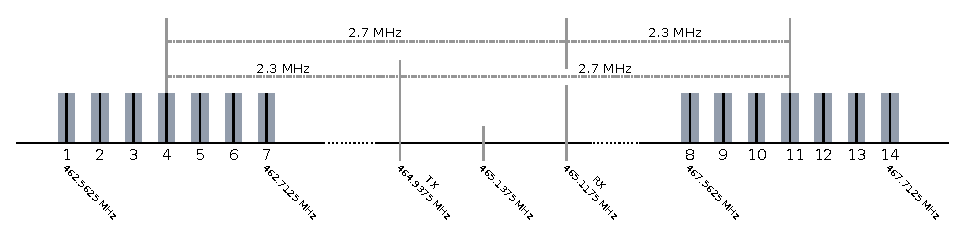
\includegraphics{images/frs/tuning.eps}
  \caption{Transceiver tuning with respect to FRS channel allocations}
  \label{fig:tuning}
\end{figure}

\begin{figure}[h]
  \centering
  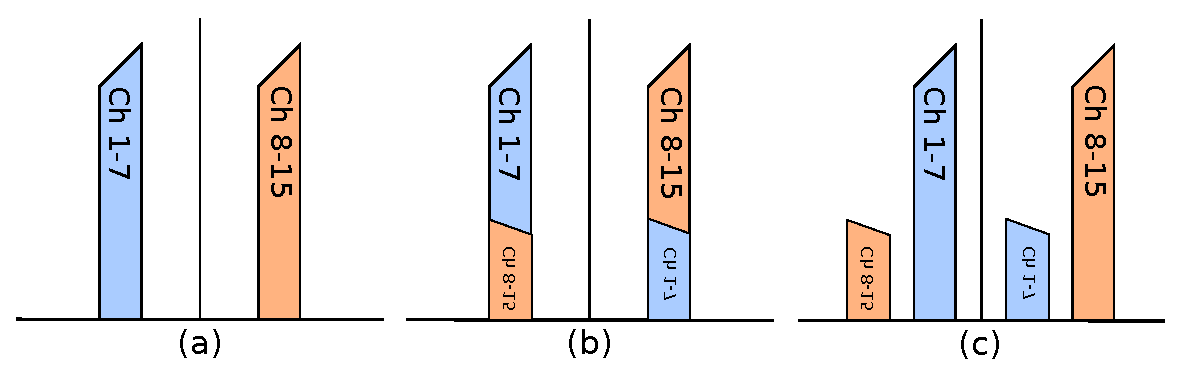
\includegraphics[width=6in]{images/frs/iq_imbalance_offset_tuning.eps}
  \\
  \footnotesize{
    (a) Nominal case: Tuning to ``center'' and no IQ imbalance.\\
    (b) Realistic case: IQ imbalance yields mirror images interfering with signals.\\
    (c) Offset tuning to ensure IQ imbalance images do not overlap.
  }
  \caption{Avoiding effect of IQ imbalance via offset tuning}
  \label{fig:iq_imbalance}
\end{figure}

We argue that \#1 is reasonable, given the ever increasing availability of USB 3.x controllers on modern systems.

Trade-offs \#2 and \#3 include interference and out-of-band emissions and are
therefore serious concerns. Fortunately, both DC offset and IQ imbalance can be
compensated for using hardware features of the bladeRF. In evaluating this
design, these signals will be important to measure and take note of.

In designing with this approach, we must first determine how the transmitter and
receiver will utilize the spectrum.  Given the 25 kHz separation between
channels and each channel's 12.5 kHz of bandwidth, this implies that the
bladeRF needs to be configured for a minimum bandwidth defined by the
following:

\begin{align*}
  \text{BW}_{\text{TX, min}} &=
  2 \times \left( \text{Max}\left(|F_{TX} - F_{CH1}|, |F_{TX} - F_{CH14}|\right) + 6.25 \,\text{kHZ} \right) \\
  &= 2 \times \left( \text{Max}\left(|464.9375 - 462.5625|, |464.9375 - 467.7125|\right) \, \text{MHz} + 6.25 \,\text{kHZ} \right) \\
  &= 5.5625 \, \text{MHz}
\end{align*}

The equation for $\text{BW}_{\text{RX, min}}$ is similar, but instead uses an
($F_{RX} = 465.1175 \,\text{MHz}$) term.

The Lime Microsystems LMS6002D transceiver \cite{LMS6002D_OVERVIEW} on the bladeRF has
discrete TX \ac{LPF} bandwidth settings, with the next largest value being 6.0
MHz in quadrature, which passes $[-3 \,\text{MHz}, 3 \,\text{MHz}]$ at baseband. The
rejection of the LMS6002D 3 MHz filter exceeds 50 dB at approximately $\pm$ 4
MHz \cite{LMS6002D_DATASHEET}. On RX, this filter is used as an anti-aliasing filter
to ensure incoming signals outside of the sampling bandwidth are sufficiently
attenuated before being converted by the ADC.  On TX, this filter is used to
remove the images created due to the zero-order hold nature of the DAC.
Therefore, to avoid these artifacts, an 8 MHz sample rate is used by the
\ac{TX} and \ac{RX} modules.

These sample rate and bandwidth calculations provide constraints which guide
the design of the \ac{TX} and \ac{RX} paths detailed in the following subsections.

MATLAB's \texttt{fdatool}, shown in Figure \ref{fig:fdatool} is used to design
the digital filters presented in this document. However, GNU Radio's
\texttt{gr\_filter\_design} program and/or Octave could also be used.

\begin{figure}[h]
  \centering
  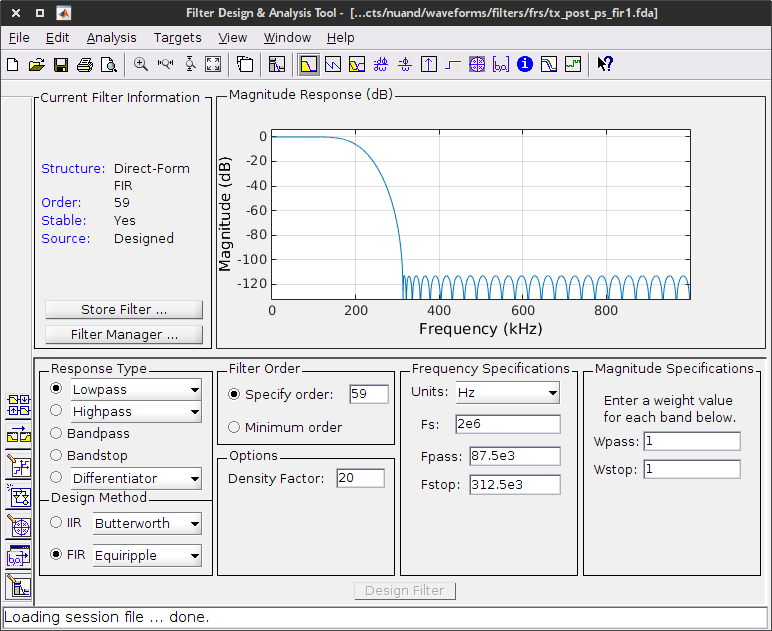
\includegraphics[width=5in]{images/fdatool.png}
  \caption{MATLAB Filter Design and Analysis Tool}
  \label{fig:fdatool}
\end{figure}

\cleardoublepage

\subsection{Transmit Path}

\subsubsection{Audio Input}
At the beginning of the TX path, audio enters through an \texttt{Audio Source}
block. Through the use of the ``pulse'' argument provided to this block, the
audio from the host machine's PulseAudio \cite{PULSE_AUDIO} subsystem is used.
A 25 kHz sample rate is selected
since it shares all common factors with the final DAC output sample  rate of 8 MHz.
This alleviates the need for digital resampling in the flowgraph prior to entering
a downstream \texttt{Polyphase Synthesizer} block.

\begin{figure}[h]
  \centering
  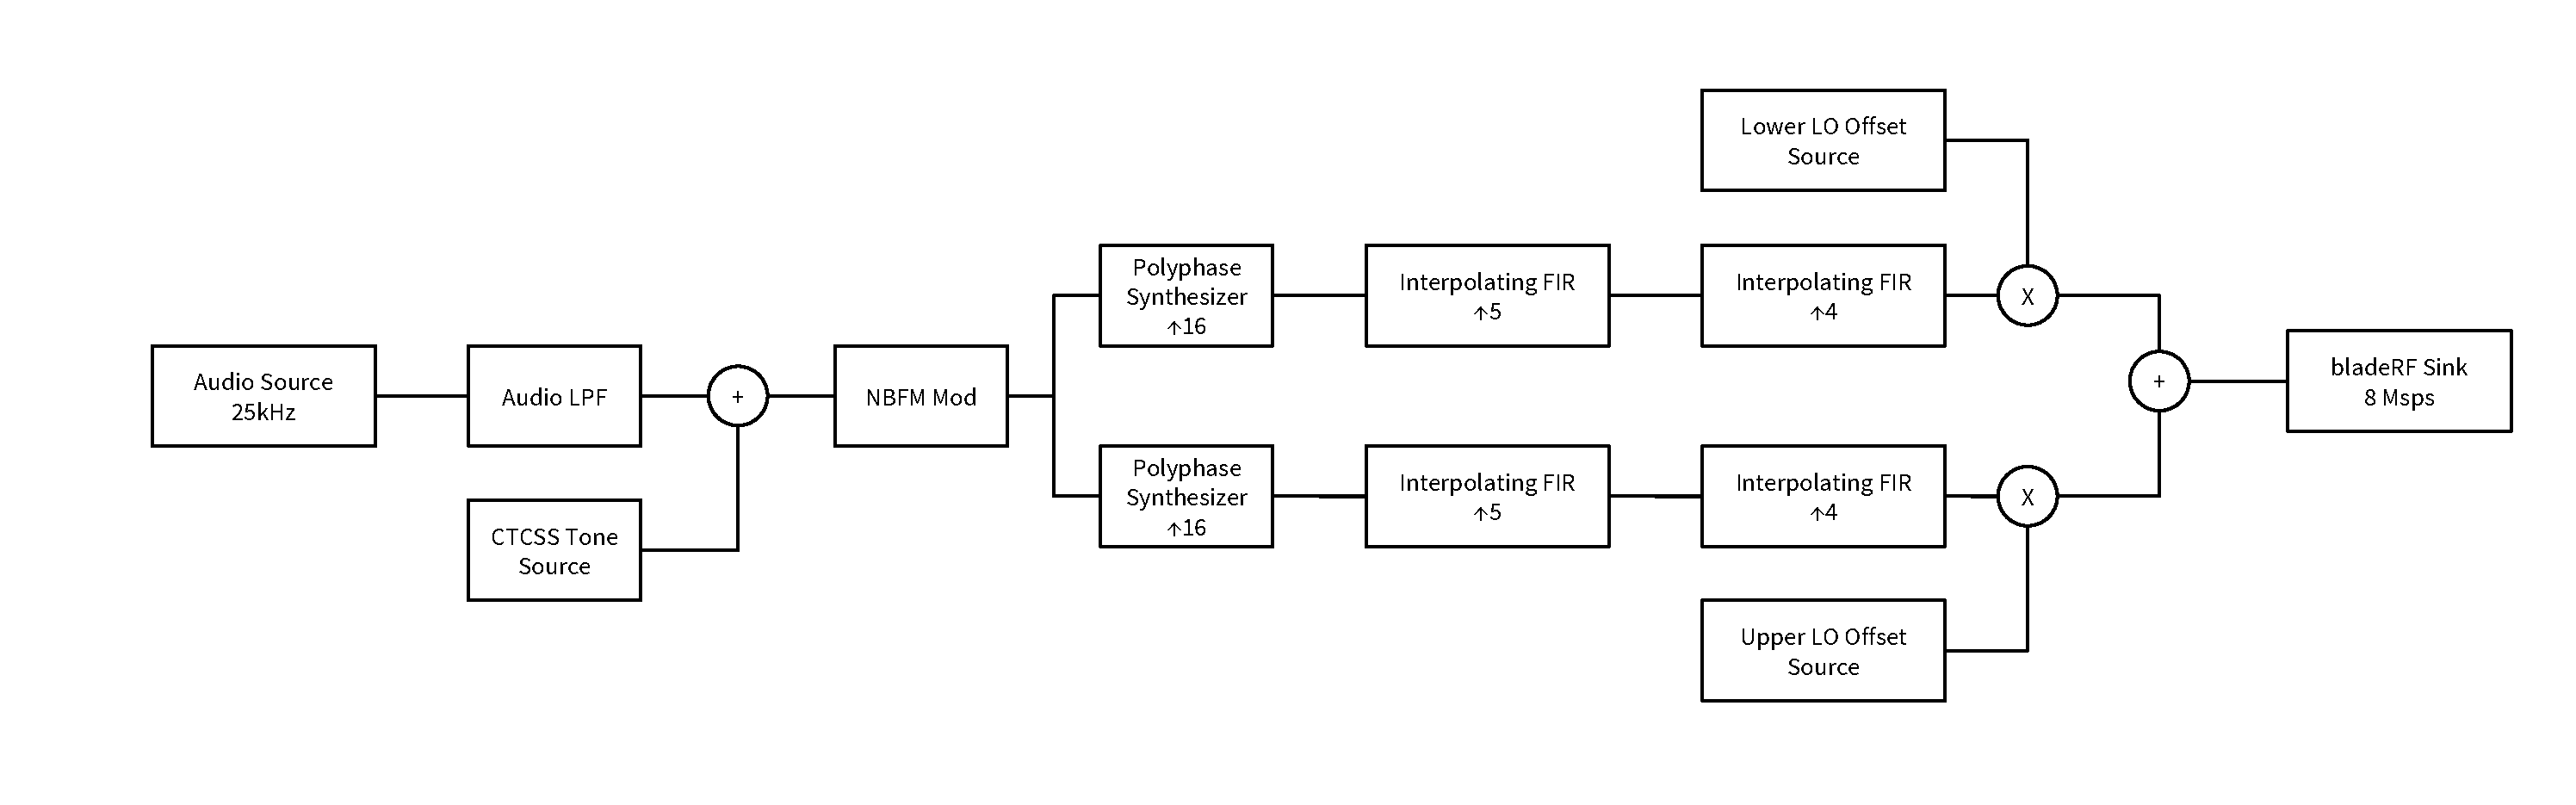
\includegraphics[width=6.5in]{images/frs/bladeRF_FRS_TX_block_diagram.pdf}
  \caption{FRS TX block diagram}
  \label{fig:frs_tx_block_diagram}
\end{figure}

A \texttt{Valve} block is used to start and stop the flow of samples to the
downstream portions of the flowgraph. This value is ``closed'' when the user
presses the ``Push to Talk'' \ac{GUI} button or checks the ``Continuous \ac{TX}'' checkbox.
When the valve is opened, downstream blocks are not processing samples which
saves CPU cycles when the transmit functionality is not enabled. When no channels
are selected to transmit, the bladeRF's \ac{TX} front end is turned off.  This
helps guarantee no residual carrier is being transmitted when there is nothing
to transmit.

A \texttt{\ac{FIR} Filter} block is used to realize an \ac{LPF} to limit the
audio frequency response to 3.125 kHz \cite{FCC_PART_95B}. Using
\texttt{fdatool} and the parameters shown in Table \ref{tab:filt_tx_audio},
a filter whose magnitude response is shown in Figure \ref{fig:filtresp_tx_audio}
is created.  From this filter's magnitude response, is is clear that
frequencies above the 3.125 kHz limit are attenuated by 60 dB, while the vast
majority of the human vocal range is passed.

\begin{table}[h]
  \centering
  \caption{Filter parameters of TX audio LPF}
  \label{tab:filt_tx_audio}
  \footnotesize
  \begin{tabular} {|l|l|}
    \hline
    \textbf{Design Method}              & FIR: Equiripple \\ \hline
    \textbf{Density Factor}             & 20              \\ \hline
    \textbf{Order}                      & 74              \\ \hline
    \textbf{Sampling Frequency (kHz)}   & 25              \\ \hline
    \textbf{Passband Frequency (kHz)}   & 2               \\ \hline
    \textbf{Stopband Frequency (kHz)}   & 3.125           \\ \hline
    \textbf{Passband Weight}            & 1               \\ \hline
    \textbf{Stopband Weight}            & 1               \\ \hline
  \end{tabular}
\end{table}

\begin{figure}[h!]
  \centering
  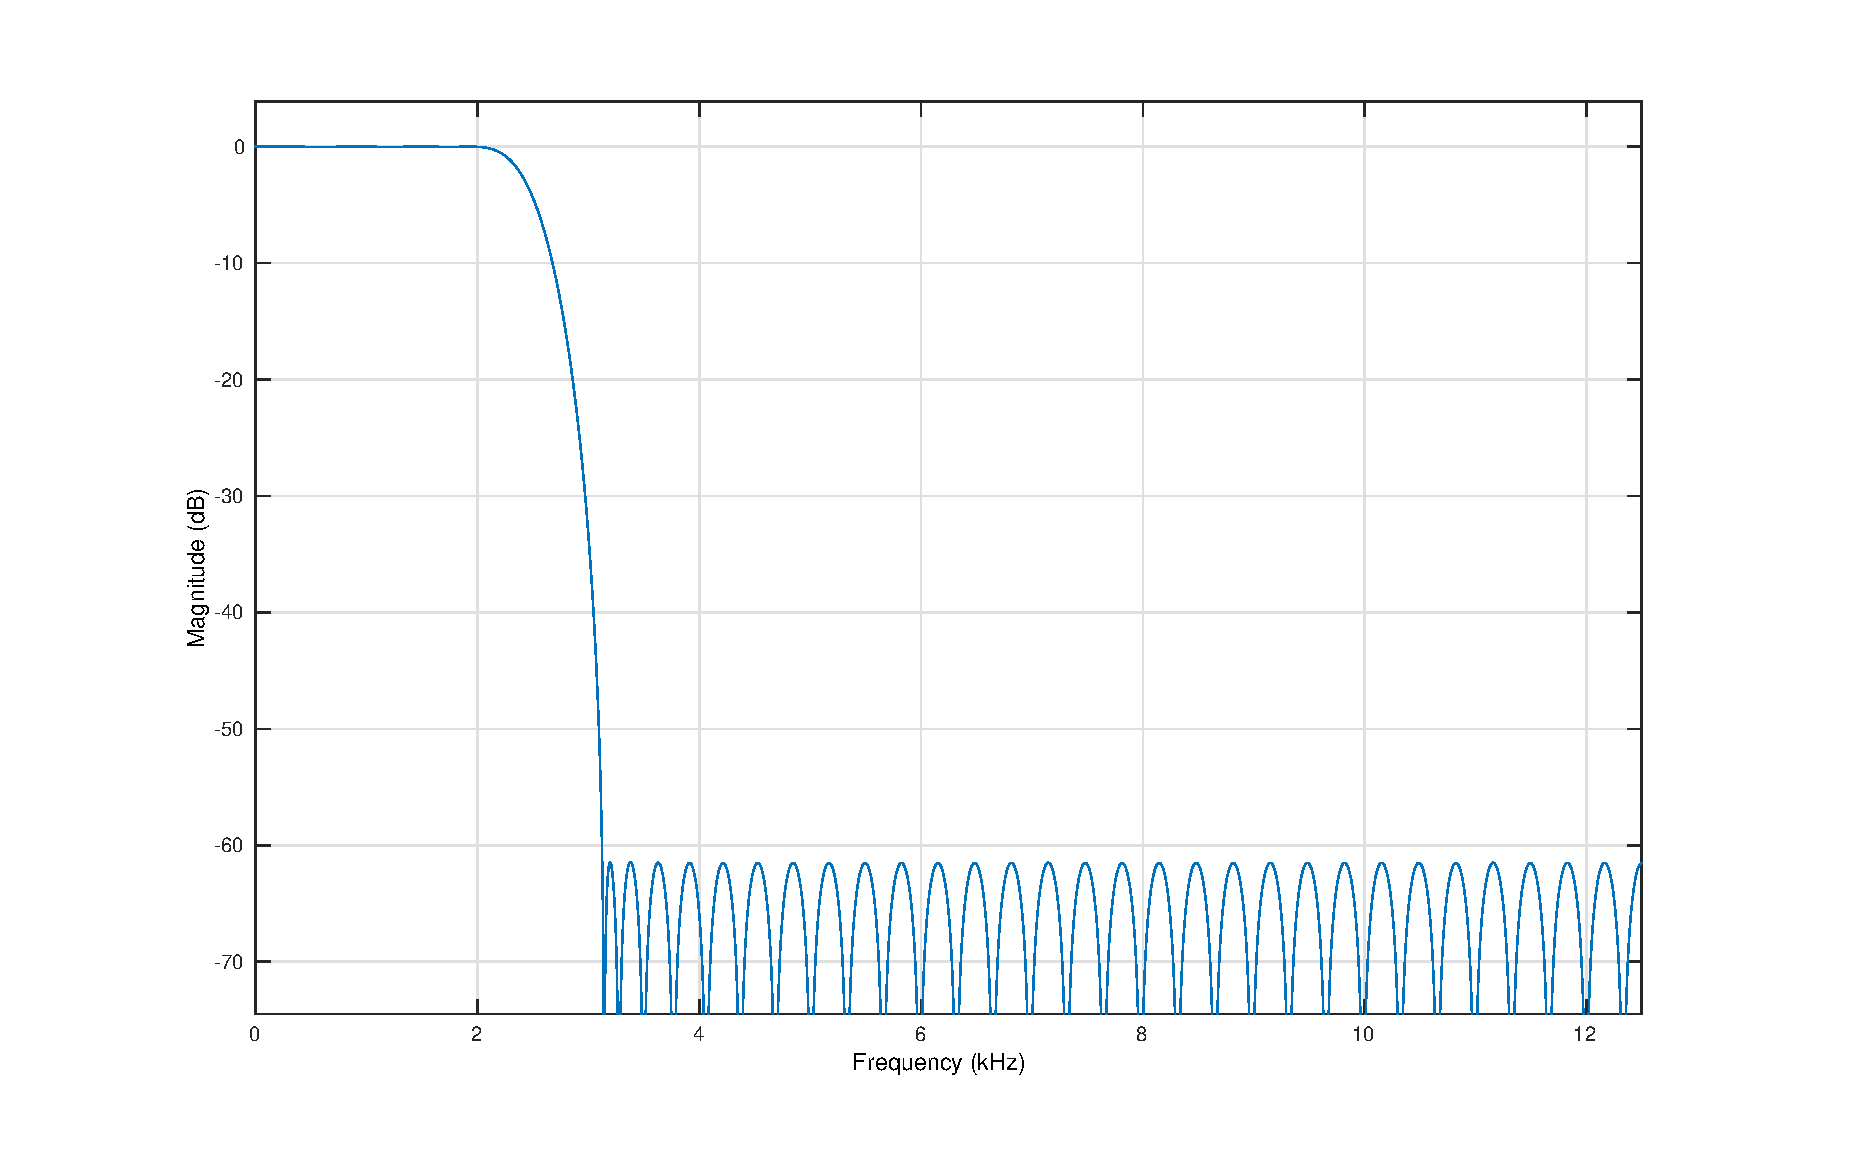
\includegraphics[width=5in]{images/frs/filter/tx/audio-fir.eps}
  \caption{Magnitude response of TX audio LPF}
  \label{fig:filtresp_tx_audio}
\end{figure}

\subsubsection{Optional CTCSS Tone}

Next, a \texttt{Selector} block is used to pass either the audio, or the audio
added with a sub-audible \ac{CTCSS} tone supplied by a \texttt{Signal Source} block, to the
next stage. The frequency of the \ac{CTCSS} tone is controlled by a drop-down
widget in the GUI.  When ``None'' is selected, the selector passes the audio
from the Audio Source block.  Otherwise, the \texttt{Signal Source} block is
configured for the desired \ac{CTCSS} frequency, and the \texttt{Selector}
passes the combination of the audio and this tone.

\subsubsection{FM Modulation and Mute Blocks}

The output of the \texttt{Selector} is fed into the \texttt{NBFM Transmit} block.
There is no need to interpolate here, so the \textit{Quadrature Rate} is left
the same as the sample rate of the incoming audio.

No pre-emphasis is desired. As of GNU Radio commit \texttt{ee369b92}
(2015-03-04), the \texttt{NBFM Transmitter} block does not currently implement
pre-emphasis\footnote{The IIR filter is constructed with hard-coded
feed-forward and feed-back taps set to 1.0.}, so the \textit{tau} parameter
is unused.  However, this \textit{tau} value is used simply to match the value
used on the RX side of the flowgraph, should this change in the future. The
rationale for this value is discussed in Section \ref{sec:fm_demod}.

The FM modulated signal is then fed into a series of \texttt{Mute} blocks. Each
of these blocks is associated with one of the \ac{FRS} channels, and is
controlled by a \ac{GUI} checkbox. When the channel is not muted, the FM modulated
signal is passed to the next stage. When muted, values of $(0 + 0j)$ are
supplied to the next stage. Note the important difference here between the
\texttt{Mute} and \texttt{Valve} blocks -- the former zeroes samples and keeps
the stream running, whereas the latter stops the flow of samples entirely.
Using a \texttt{Valve} here would cause the following block to stop running if
one or more channels were muted, which is undesirable.

\subsubsection{Polyphase Synthesizer} \label{sec:polysynth}
Because the \ac{FRS} channels within their groupings are evenly spaced,
GNU Radio's \texttt{Polyphase Synthesizer} \cite{TRONDEAU_PFB} provides a very
simple solution for combining multiple channels into a single interpolated signal.

Two \texttt{Polyphase Synthesizer} blocks are used in conjunction with each other to
construct two 400 kHz wide signals -- one containing \ac{FRS} channels 1-7, and a second
400 kHz wide signal containing \ac{FRS} channels 8-14. Channels 4 and 11 are
located at the center frequencies of their respective signals. Each channel in
the output is separated by the desired 25 kHz, as this is the input sample rate.

As noted in the previous section, input channels contain either the FM
modulated audio signal, or $(0 + 0j)$, depending on the state of the associated
\texttt{mute} block.

\begin{figure}[h!]
  \centering
  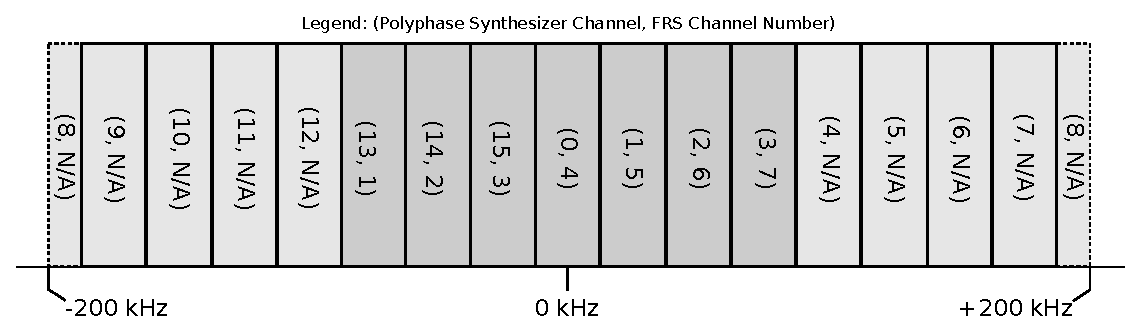
\includegraphics[scale=0.85]{images/frs/polyphase_synth_ch1-7.eps}
  \caption{Polyphase Synthesizer configuration for FRS channels 1-7}
  \label{fig:polyphasesynth}
\end{figure}

Although only 7 of these 25 kHz channels are required, these blocks are
configured for a total of 16 channels, with 9 of the channels left unused. This
is done to alleviate the need for more interpolation in later blocks; a
value of ``16'' is selected to avoid necessitating an additional factor of 2
in later interpolating blocks.  The extra unused channels
allow for a wider transition band to be used in the interpolating \ac{FIR}
filter that follows this stage, which reduces the required number of filter
taps\footnote{This reduces the number of convolution operations required.}.

The \textit{Channel Map} property is set to \texttt{[13, 14, 15, 0, 1, 2, 3]},
in order to position \ac{FRS} channels 1-7 (on input indices 0 through 6)
as shown in Figure \ref{fig:polyphasesynth}. With respect to channel mapping,
the same approach is taken for \ac{FRS} channels 8 through 14 in the second
\texttt{Polyphase Synthesizer} block.

To minimize the impact of aliases, the \texttt{Polyphase Synthesizer} applies
a per-channel filter at the output sample rate of 400 kHz. The filter used in
this block passes signals within the 12.5 kHz \ac{FRS} bandwidth limit.
Therefore, the pass band is located at $\frac{12.5}{2} \, \text{kHz}$.
To reject the image occurring at the next channel, the stop band is place before
the ``edge'' of the image, expected to occur at $18.75 \,\text{kHz} = 25
\,\text{kHz} - \frac{12.5}{2} \,\text{kHz}$.

The parameters used with \texttt{fdatool} to generate these
filter taps are shown in Table \ref{tab:tx_polysynth}. As shown by the magnitude
response in Figure \ref{fig:filtresp_tx_ps}, spectral content outside of the
desired region should be significantly rejected.

\begin{table}[h]
  \centering
  \caption{Filter parameters for polyphase synthesizer LPF}
  \label{tab:tx_polysynth}
  \footnotesize
  \begin{tabular} {|l|l|}
    \hline
    \textbf{Design Method}              & FIR: Equiripple \\ \hline
    \textbf{Density Factor}             & 20              \\ \hline
    \textbf{Order}                      & 191             \\ \hline
    \textbf{Sampling Frequency (MHz)}   & 400             \\ \hline
    \textbf{Passband Frequency (kHz)}   & 6.25            \\ \hline
    \textbf{Stopband Frequency (kHz)}   & 18.75           \\ \hline
    \textbf{Passband Weight}            & 1               \\ \hline
    \textbf{Stopband Weight}            & 1               \\ \hline
  \end{tabular}
\end{table}

\begin{figure}[h]
  \centering
  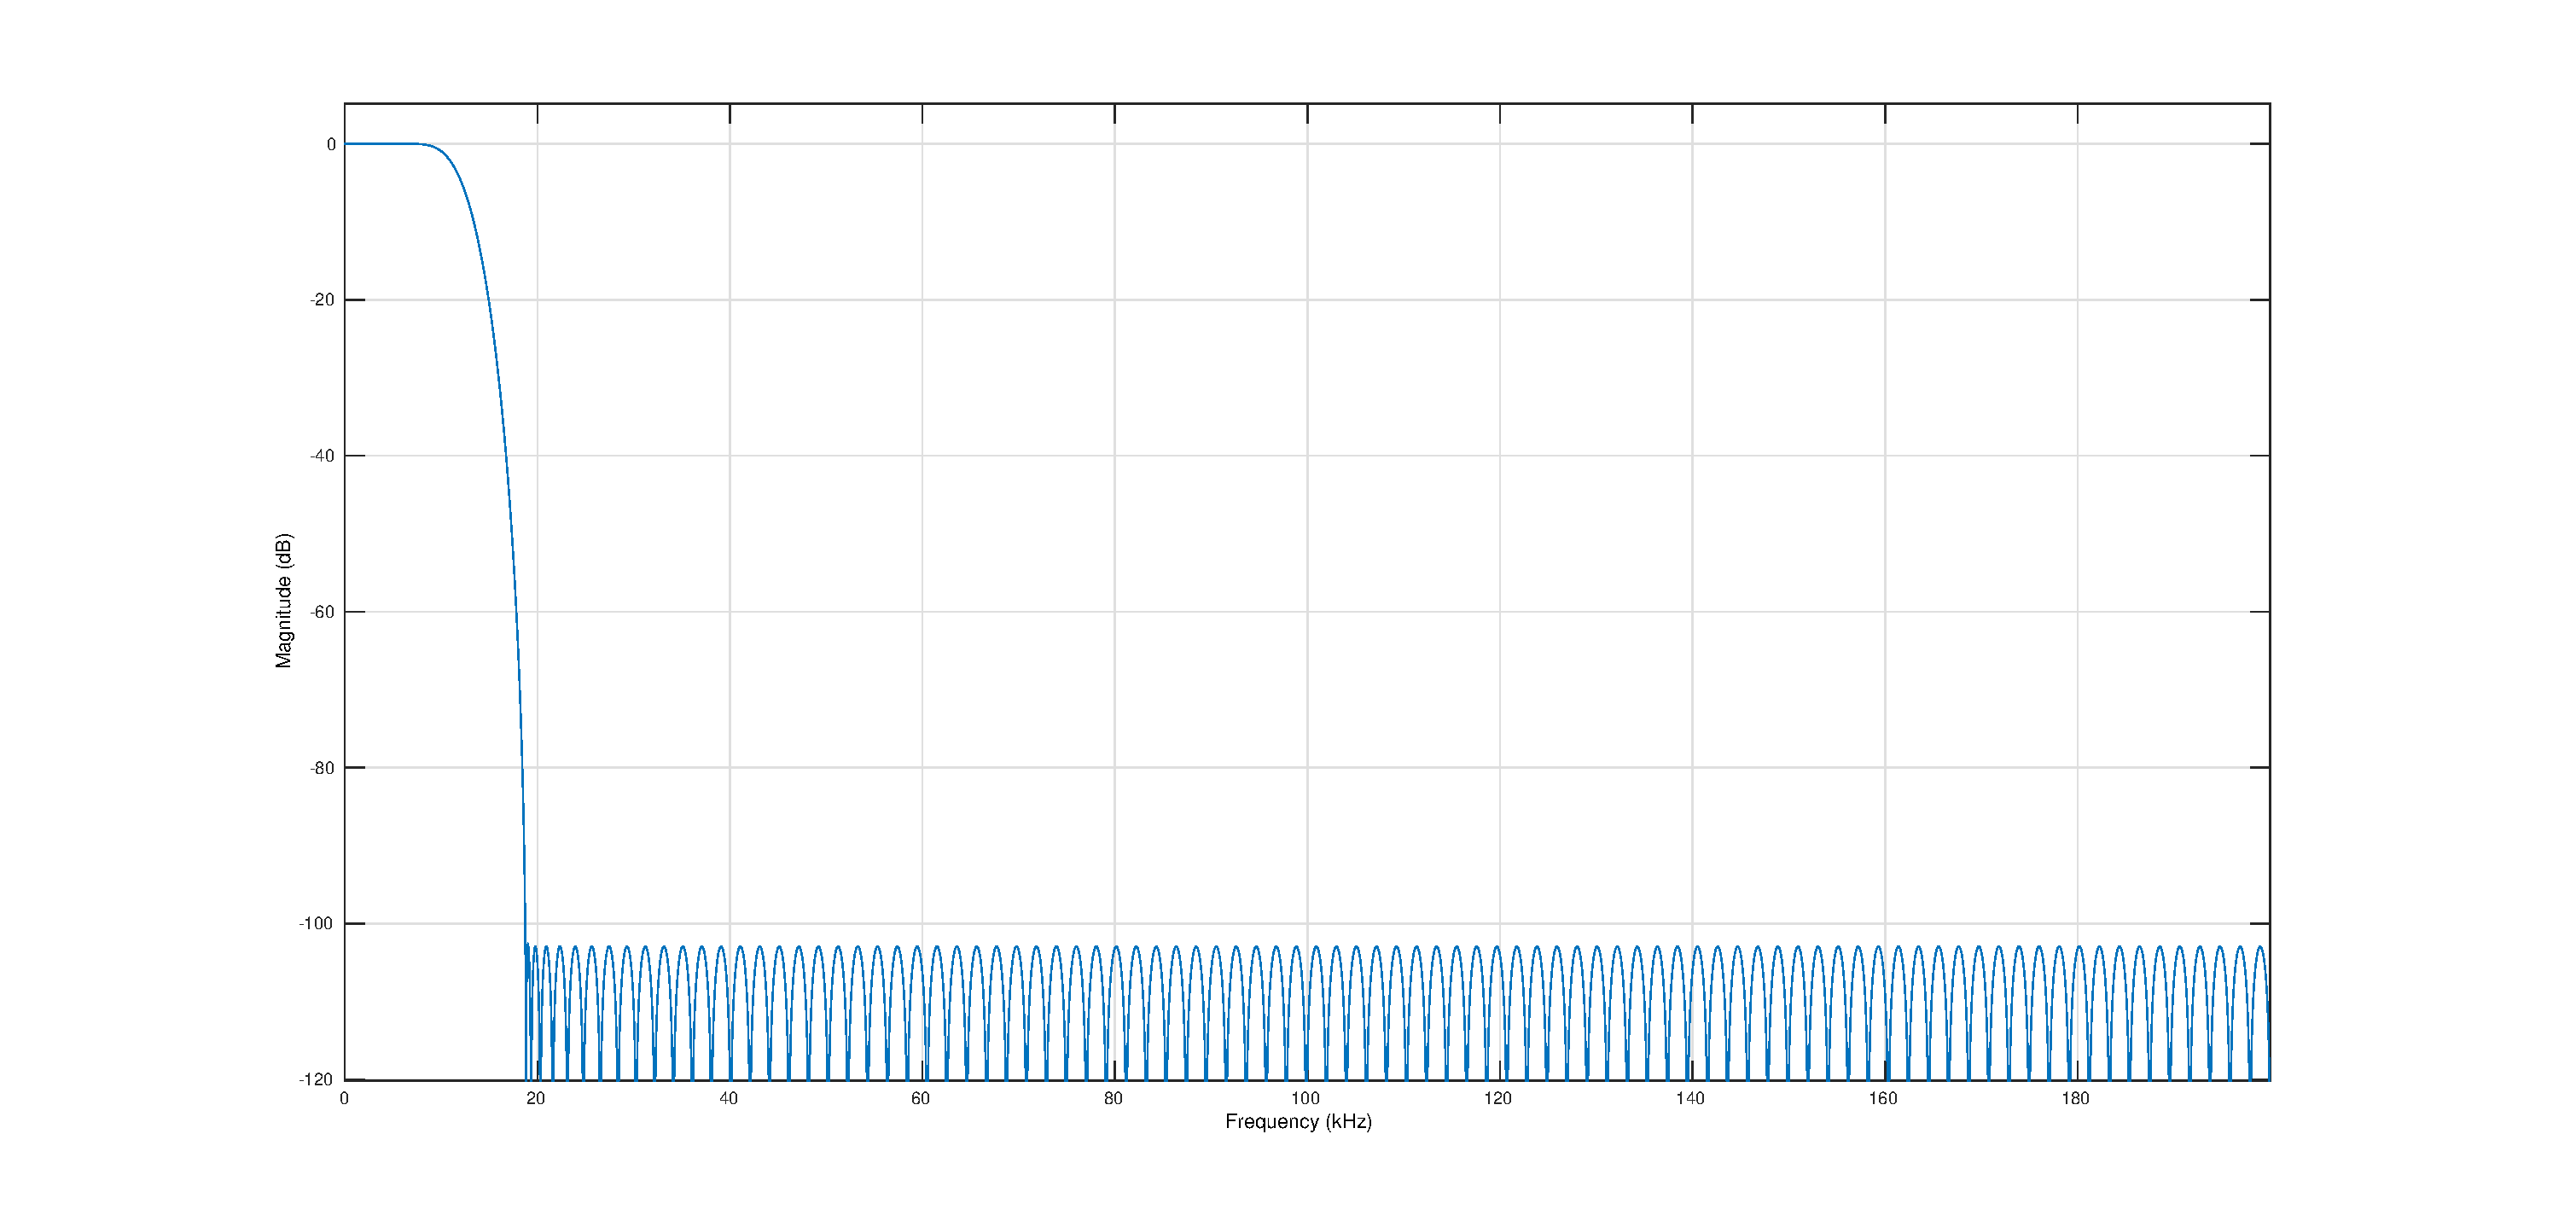
\includegraphics[width=6in]{images/frs/filter/tx/polyphase-synth-fir.eps}
  \caption{Magnitude response of polyphase synthesizer FIR filter}
  \label{fig:filtresp_tx_ps}
\end{figure}

The outputs of these blocks are connected to \texttt{Qt GUI Waterfall Sink}
blocks to provide feedback to the user that the channels selected via
checkboxes are indeed being transmitted on, as well as a confirmation of the
signal bandwidth.

\subsubsection{Interpolating Filters}

Ultimately, the two groups of \ac{FRS} signals must be recombined into a single
signal that has been interpolated by a factor of 20 to match the hardware's 8 Msps
sample rate.  This interpolation is achieved utilizing two
\texttt{Interpolating \ac{FIR} Filter} blocks. As indicated by the block name,
these first interpolate by zero-stuffing samples and then filter to reject
image artifacts that result from zero-stuffing.

The first \ac{FIR} filter interpolates by a factor of 5, yielding an output
sample rate of 2 MHz. The second stage interpolates by a factor of 4, yielding
the final output sample rate of 8 MHz.

The parameters for these filters are shown in Tables \ref{tab:tx_interp_fir1}
and \ref{tab:tx_interp_fir2}.

To account for energy lost due to the interpolation, the filter taps obtained
via \texttt{fdatool} are scaled by their associated interpolation factor. Figure
\ref{fig:tx_interp_firs} presents the magnitude responses of the individual
stages, as well the combined response of both stages.

The passband frequencies are selected to ensure all 7 of the 25 kHz channels
are passed without attenuation. Of the 400 kHz of bandwidth provided to the
input of the first filter, 175 kHz\footnote{Recall that seven 25 kHz inputs
are provided to the \texttt{Polyphase Synthesizer}.} may contain information.
Therefore, we set our passband to $85.7 \, \text{kHZ} = \frac{175}{2}
\,\text{kHz}$.

The stop band for the first filter is placed at the location where the first
image artifact caused by interpolation is expected to be. This is calculated as
follows:
\begin{align*}
  F_{\text{stop}} &= \frac{F_s}{2} + \left( \frac{F_s}{2} - \text{BW} \right) \\
  &= 200 \,\text{kHz} + \left( 200 \,\text{kHz} - 87.5 \,\text{kHz} \right) \\
  &= 312.5 \,\text{kHz}
\end{align*}

The position of the second filter's stop band is selected such that the first
null of this filter aligns with null occurring before the image of the previous
filter's response. This can be quickly achieved through an iterative process of
measuring the location of the first null, changing the $F_{\text{stop}}$ value
in \texttt{fdatool}, and repeating until the nulls align sufficiently.

\begin{table}[h]
  \centering
  \caption{Filter parameters for first TX interpolating (5x) FIR filter}
  \label{tab:tx_interp_fir1}
  \footnotesize
  \begin{tabular} {|l|l|}
    \hline
    \textbf{Design Method}              & FIR: Equiripple \\ \hline
    \textbf{Density Factor}             & 20              \\ \hline
    \textbf{Order}                      & 59              \\ \hline
    \textbf{Sampling Frequency (MHz)}   & 2               \\ \hline
    \textbf{Passband Frequency (kHz)}   & 87.5            \\ \hline
    \textbf{Stopband Frequency (kHz)}   & 312.5           \\ \hline
    \textbf{Passband Weight}            & 1               \\ \hline
    \textbf{Stopband Weight}            & 1               \\ \hline
  \end{tabular}
\end{table}

\begin{table}[h]
  \centering
  \caption{Filter parameters for second TX interpolating (4x) FIR filter}
  \label{tab:tx_interp_fir2}
  \footnotesize
  \begin{tabular} {|l|l|}
    \hline
    \textbf{Design Method}              & FIR: Equiripple \\ \hline
    \textbf{Density Factor}             & 20              \\ \hline
    \textbf{Order}                      & 27              \\ \hline
    \textbf{Sampling Frequency (MHz)}   & 8               \\ \hline
    \textbf{Passband Frequency (kHz)}   & 87.5            \\ \hline
    \textbf{Stopband Frequency (MHz)}   & 1.67            \\ \hline
    \textbf{Passband Weight}            & 1               \\ \hline
    \textbf{Stopband Weight}            & 1               \\ \hline
  \end{tabular}
\end{table}

\begin{figure}[h]
  \centering
  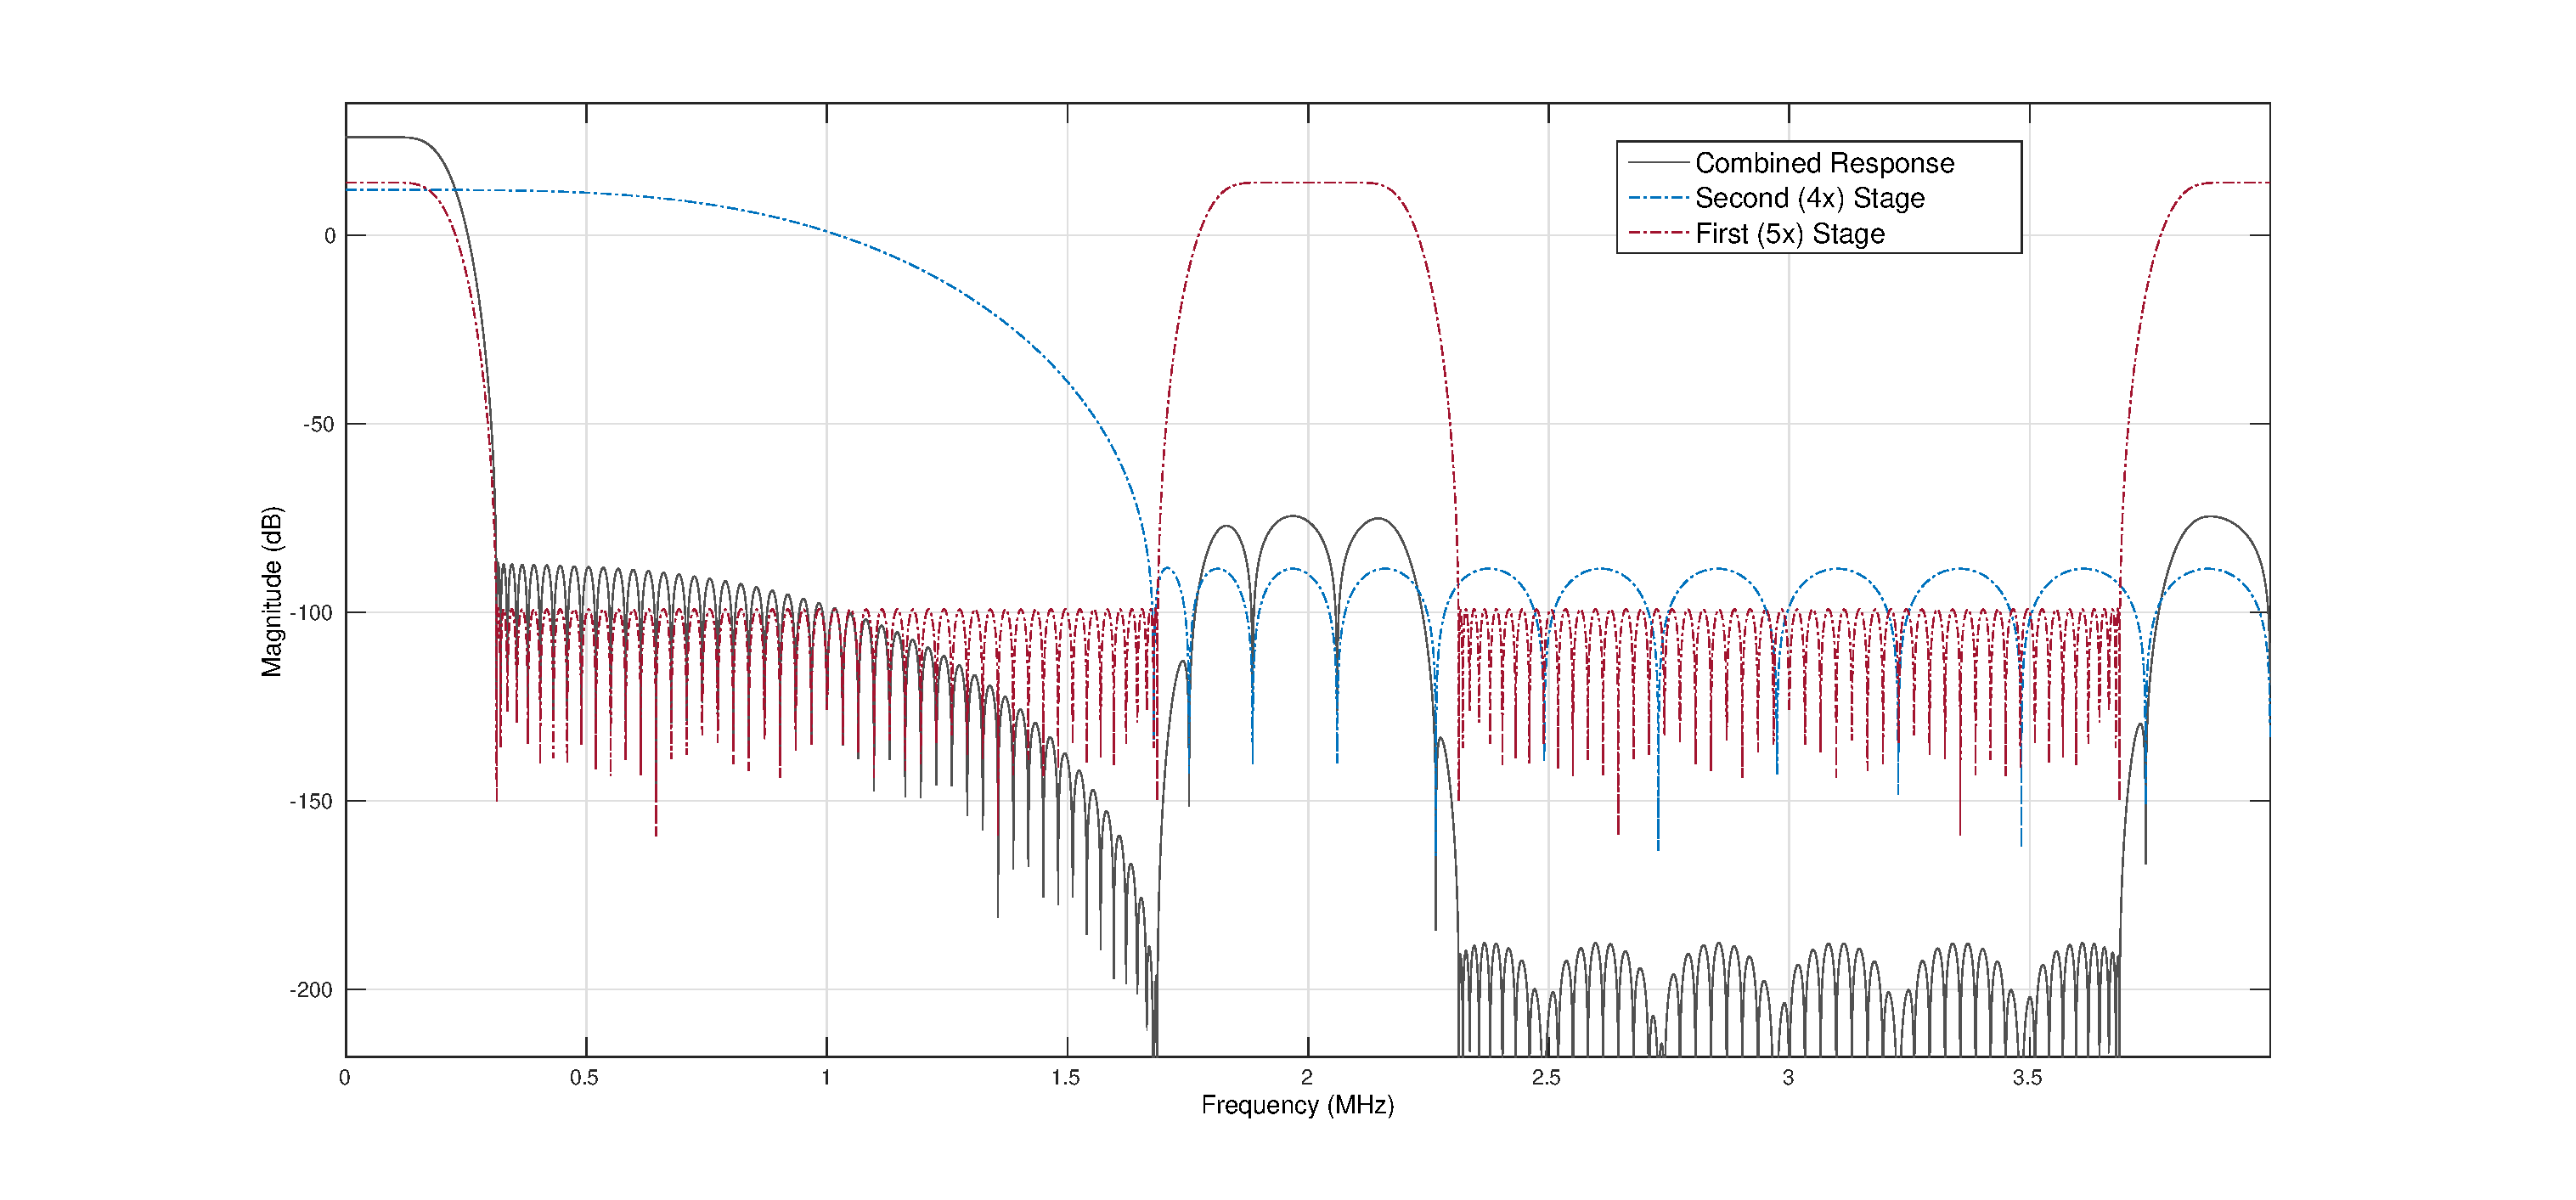
\includegraphics[width=6.5in]{images/frs/filter/tx/interp-firs.eps}
  \caption{Magnitude response TX interpolating FIR filters}
  \label{fig:tx_interp_firs}
\end{figure}

The motivation behind using two stages rather than one is to minimize the
number of convolution operations performed by the filter per unit of time.
If a single interpolation by 20 were performed, all of the filtering would
be done at the final 8 MHz samplerate. Because the \ac{FRS} spectral content is in a relatively
small percentage of the interpolated signal, this requires a large number
of taps to achieve the desired transition band and rejection. This combination
of higher sample rate and more taps leads to higher computational load.
In general, by performing the interpolation and filtering in stages, it is
possible to achieve fewer operations per stage, with each stage running at a
fraction of the final sample rate.

\subsubsection{Mixing and Hardware Sink}

After the previous stages of interpolation, there is ample bandwidth to combine
the two groups of 7 \ac{FRS} channels. Each group is mixed from baseband to
a target frequency offset, per Figure \ref{fig:tuning}, and then added to form
the final output signal. This mixing is performed though multiplication with
the output of a \texttt{Signal Source} block.

The \texttt{Signal source} is configured to provide a cosine at the target
offset frequency (-2.3 MHz for Ch 1-7 and 2.7 MHz for Ch 8-14). The amplitude
of this cosine is set to 0.5 in order to ensure that the final output is within
(-1.0, 1.0).

The final output signal is sent to the bladeRF via an \texttt{osmocom Sink}
block, which presents a hardware-agnostic sink interface. 

The sink's frequency, sample rate, and bandwidth are set to the values
described at the beginning of this section -- 464.9375 MHz, 8Msps, and 6 MHz,
respectively.

The bladeRF has two \ac{VGA} stages in its \ac{TX} path, as shown in
\cite{LMS6002D_DATASHEET}. Generally, TXVGA1 should be increased before
TXVGA2. Sliders for these parameters have been provided in the \ac{GUI}, via
\texttt{QT GUI Range} block. The \texttt{osmocom Sink} block maps its
\textit{BB Gain} to TXVGA1, and the \textit{RF Gain} to TXVGA2.

The device-specific arguments are provided via the \textit{Device Parameters}
property string, which includes the following:

\begin{center}
  \texttt{bladerf=0,buffers=128,buflen=8192,transfers=32}
\end{center}

The first argument specifies that the first instance of a bladeRF device found
on the system should be used. The remaining items configure properties of the
data stream, including number of sample buffers to use, the size of each sample
buffer, and the number of USB transfers to pre-allocate. Additional buffering
ensures that samples are not dropped during periods of heavy CPU load, with
trade-offs of added latency and memory usage.

\newpage
\subsection{Receive Path}

The design of the \ac{RX} path is very similar to the \ac{TX} path, but in
reverse.  The same sample rate and bandwidth settings from the \ac{TX} path are applied.
Also, the filter designs from the \ac{TX} path are used as a starting point for the
associated filter in the \ac{RX} path, implying that the decimation rates follow
the same interpolation rates.

\begin{figure}[h]
  \centering
  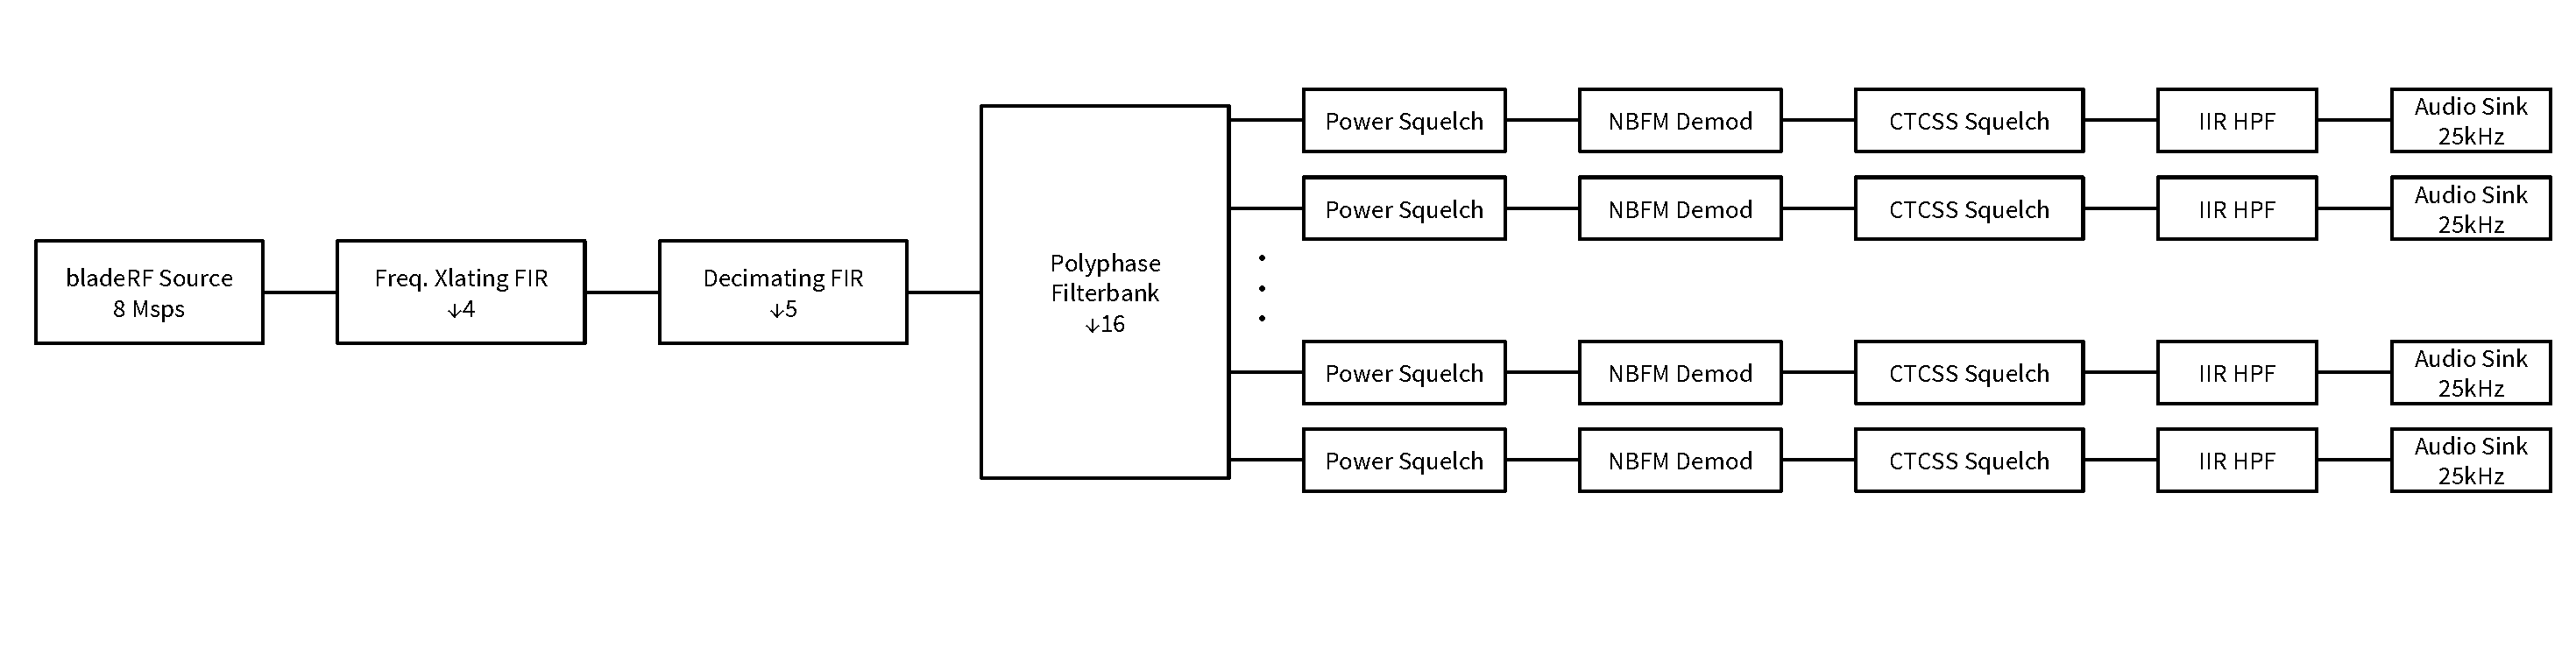
\includegraphics[width=6.5in]{images/frs/bladeRF_FRS_RX_block_diagram.pdf}
  \caption{FRS RX block diagram}
  \label{fig:frs_rx_block_diagram}
\end{figure}

\subsubsection{Hardware Source and Valve}

An \texttt{osmocom Source} block is used to receive samples from the bladeRF.
Per previous calculations, it is tuned to 465.3375 MHz, with a sample rate
of 8 Msps, and a bandwidth of 6 MHz.

In the \ac{RX} path, the LMS6002D provides a \ac{LNA} gain stage, and two
\ac{VGA} gain stages. The \ac{LNA} stage should be adjusted first, followed by
RXVGA1 and then RXVGA2. The \texttt{osmocom Source} block maps the \textit{RF
Gain} field to the \ac{LNA} gain, and the \textit{BB Gain} to the sum of RXVGA1
and RXVGA2, where RXVGA2 is incremented after RXVGA1 reaches its max value.

The output of this hardware source is connected to a \texttt{Valve} block
allowing all \ac{RX} processing to be stopped.

\subsubsection{Power Meter}
The instantaneous power of the received signal passing through the \texttt{Valve} is
filtered via a \texttt{Single Pole IIR Filter}, converted to dBFs, and then
displayed via a \texttt{QT GUI Number Sink}. This \ac{GUI} Widget provides a
thermometer-style bar that allows the user to quickly gain a sense of the input
power over the full 8 MHz captured at the ADC.

If strong in-band signals cause this \ac{GUI} item to display a value
greater than 0 dBFS, the input will saturate and likely result in artifacts
and distortion. Upon observing the power meter nearing or exceeding 0dBFS, a
user should reduce \ac{RX} gain values, or introduce external attenuation if
gain values are already at a minimum.

\subsubsection{Frequency Translation and Decimating FIR Filters}
The signals passed by the \texttt{Valve} are also routed to sections of
the flowgraph that perform frequency translation, filtering, and decimation.
Again, like in the \ac{TX} case, the decimation and filtering is performed
in two stages instead of a single stage in order to reduce computational load.

The first block is a \texttt{Frequency Xlating FIR Filter}, which efficiently
translates a signal to a desired frequency offset, while filtering and
decimating.

The \texttt{Frequency Xlating FIR Filter} for \ac{FRS} channels 1-7 centers
the input originally at -2.7MHz, and the block for channels 8-14 centers the
input originally at 2.3 MHz, per Figure \ref{fig:tuning}.

These blocks are configured to decimate by a factor of 4, yielding an output
sample rate of 2 MHz. To avoid aliasing caused by decimation, the \ac{FIR}
filter applied prior to decimation must reject frequencies outside [-1 MHz, 1
MHz]. Frequencies within [-87.5 kHz, 87.5 kHz] must be passed, as this region
of the spectrum contains the \ac{FRS} channels. The parameters used to create a
filter that meets these constraints are shown in Table \ref{tab:rx_xlat_fir}.

\begin{table}[h]
  \centering
  \caption{Filter parameters for RX frequency translating and decimating FIR filter}
  \label{tab:rx_xlat_fir}
  \footnotesize
  \begin{tabular} {|l|l|}
    \hline
    \textbf{Design Method}              & FIR: Equiripple \\ \hline
    \textbf{Density Factor}             & 20              \\ \hline
    \textbf{Order}                      & 39              \\ \hline
    \textbf{Sampling Frequency (MHz)}   & 8               \\ \hline
    \textbf{Passband Frequency (kHz)}   & 21.875          \\ \hline
    \textbf{Stopband Frequency (MHz)}   & 1               \\ \hline
    \textbf{Passband Weight}            & 1               \\ \hline
    \textbf{Stopband Weight}            & 1               \\ \hline
  \end{tabular}
\end{table}

Note that although the pass band frequency specified for use with
\texttt{fdatool} is 21.875 kHz, the resulting response of this stage (Figure
\ref{fig:rx_firs}) does not impose any significant attenuation up through
the 87.5 kHz region of interest. In this case, it is found that relaxing the
passband constraint allows \texttt{fdatool} to design a filter with better
stop band attenuation.

Next, the 2 MHz signal is passed through a \texttt{Decimating FIR Filter},
which performs filtering and an additional decimation by a factor of 5,
resulting in a 400 kHz signal. This implies that frequencies outside of
[-200 kHz, 200 kHz] must be rejected, while ensuring the \ac{FRS} content in
[-87.5 kHz, 87.5 kHz] is passed without attenuation. Table \ref{tab:rx_dec_fir}
presents the filter design parameters.

\begin{table}[h]
  \centering
  \caption{Filter parameters for RX decimating FIR filter}
  \label{tab:rx_dec_fir}
  \footnotesize
  \begin{tabular} {|l|l|}
    \hline
    \textbf{Design Method}              & FIR: Equiripple \\ \hline
    \textbf{Density Factor}             & 20              \\ \hline
    \textbf{Order}                      & 39              \\ \hline
    \textbf{Sampling Frequency (MHz)}   & 2               \\ \hline
    \textbf{Passband Frequency (kHz)}   & 87.5            \\ \hline
    \textbf{Stopband Frequency (kHz)}   & 200             \\ \hline
    \textbf{Passband Weight}            & 1               \\ \hline
    \textbf{Stopband Weight}            & 1               \\ \hline
  \end{tabular}
\end{table}

As shown in Figure \ref{fig:rx_firs}, this filter does indeed meet the
desired requirements, as does the entire response of the two filtering stages.

\begin{figure}[h!]
  \centering
  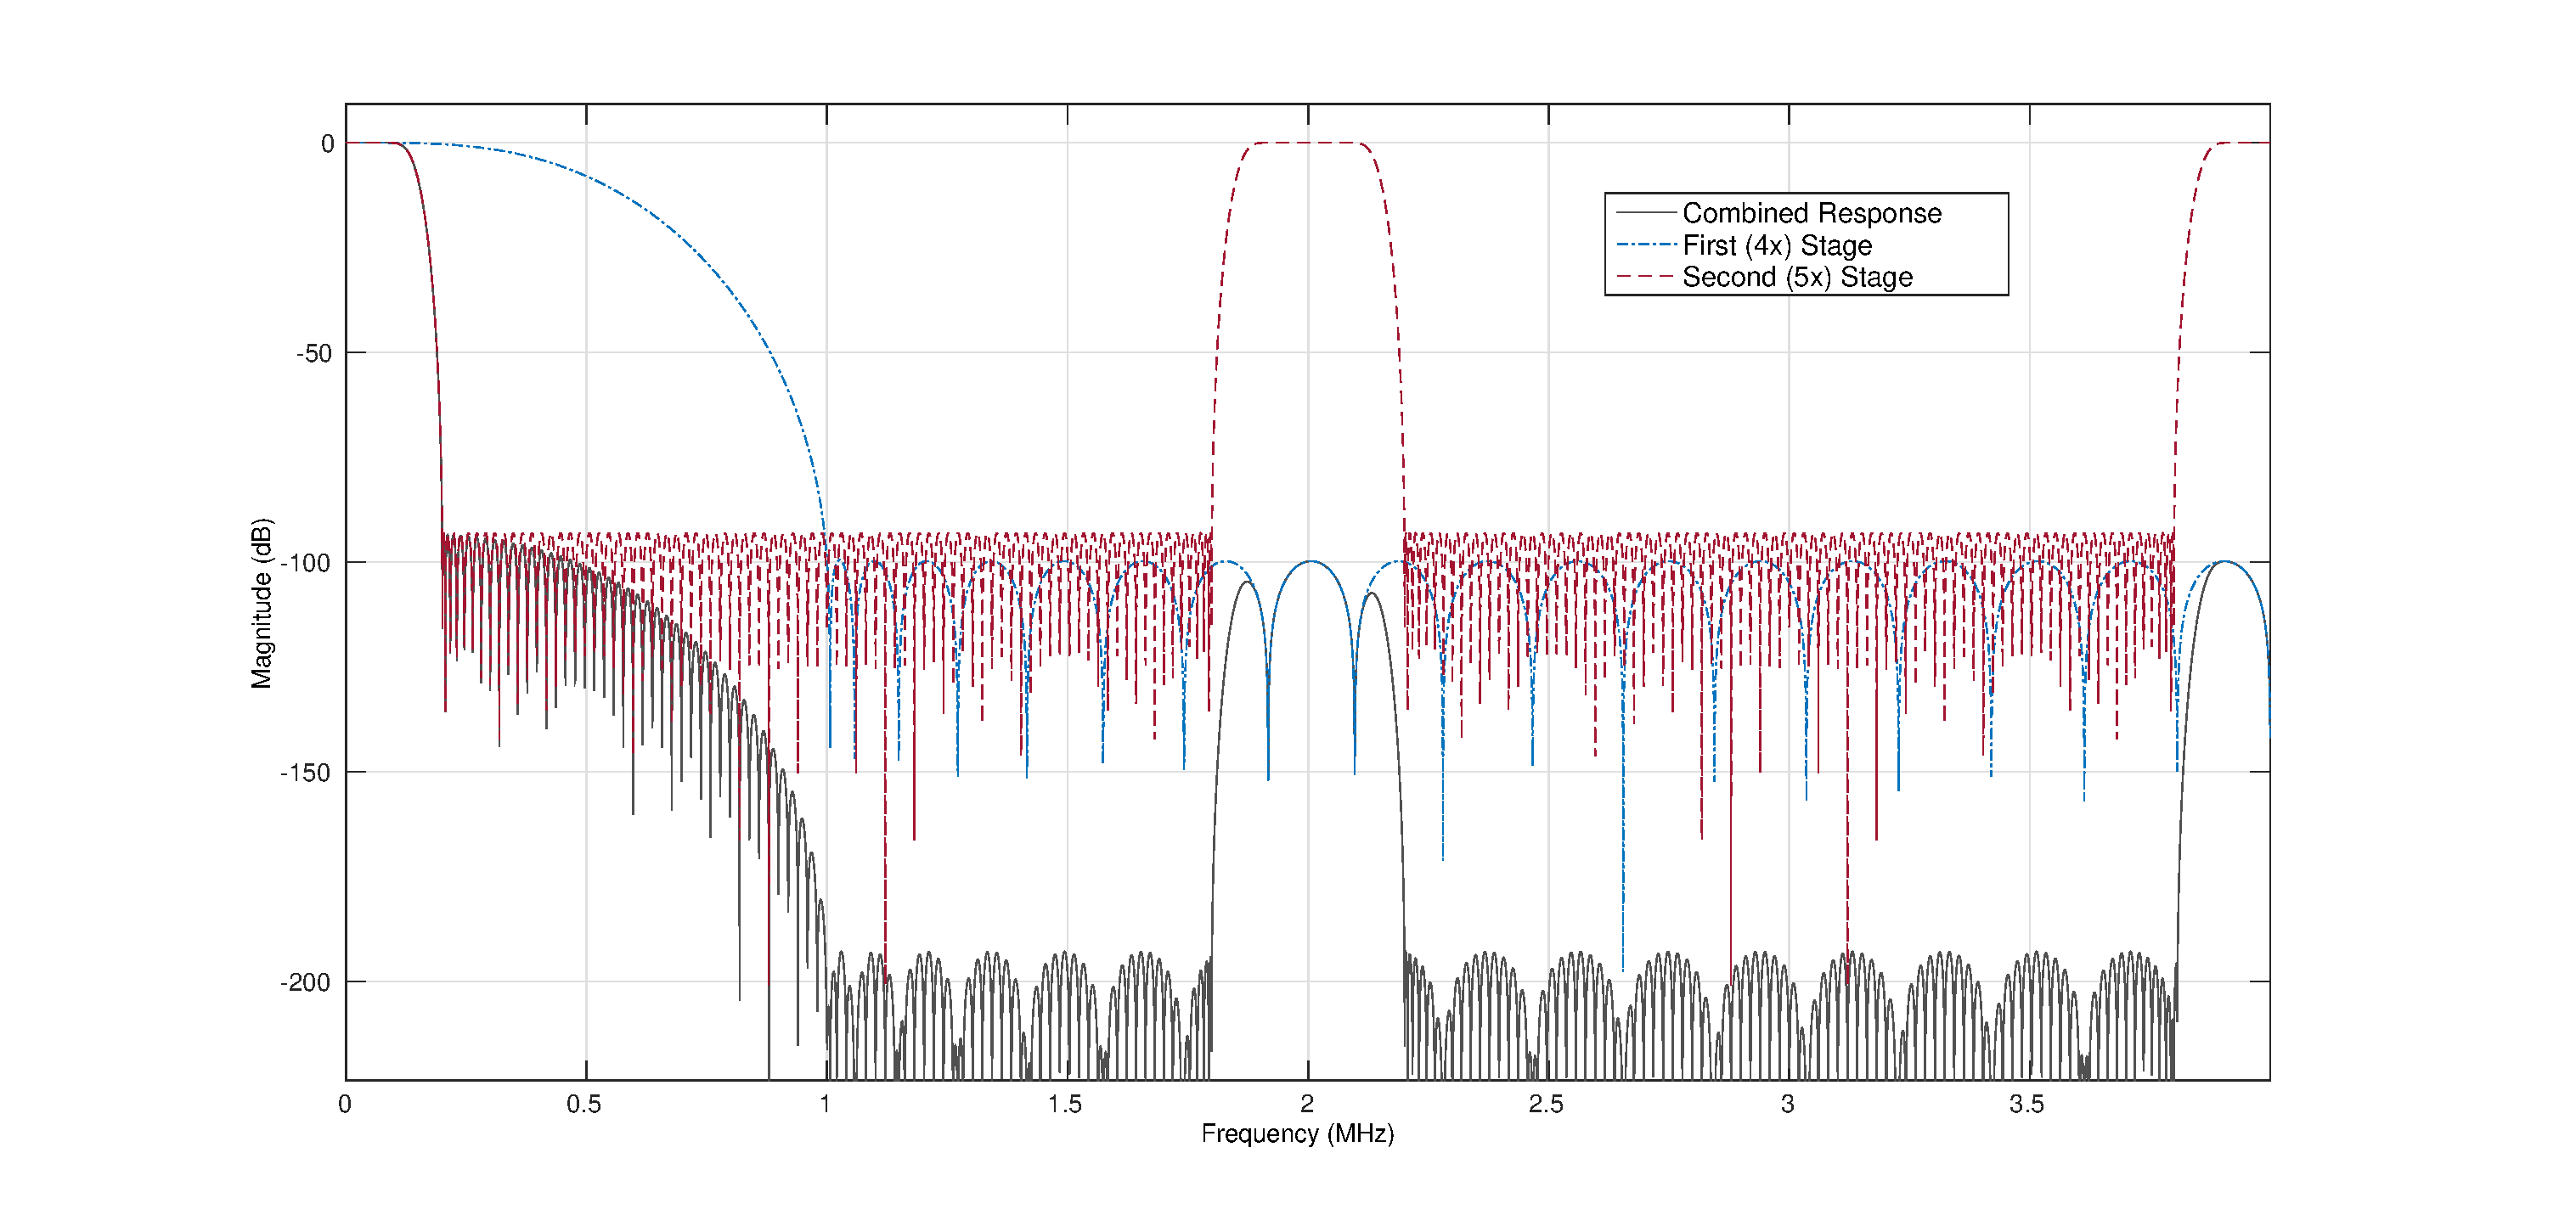
\includegraphics[width=6.5in]{images/frs/filter/rx/dec-firs.eps}
  \caption{Magnitude response of RX decimating FIR filters}
  \label{fig:rx_firs}
\end{figure}

\subsubsection{Polyphase Channelizer}

In this flowgraph, the usage of the \texttt{Polyphase Channelizer} is very
similar to that of the \texttt{Polyphase Synthesizer} in the \ac{TX} path.

The input to each channelizer is a 400 kHz wide signal, centered on \ac{FRS}
channels 4 or 11 (see Figure \ref{fig:polyphasesynth}). By configuring the
channelizer for 16 channels and using the same channel mapping presented in
Section \ref{sec:polysynth}, indices 0-6 are associated with \ac{FRS}
channels 1-7 or 8-14.

Each of the outputs containing a single \ac{FRS} channel are routed to
a \texttt{Valve} block.  Similar to the \texttt{Mute} blocks used in the \ac{TX}
path, these are controlled by \ac{GUI} checkboxes to allow the user to select which
\ac{FRS} channels to listen to. However, the \texttt{Valve} is used
to disable downstream blocks when opened. This eliminates the unnecessary
processing of channels that the user is not interested in.

Bus ports \cite{TRONDEAU_BUSPORT} are used to route the remaining 9 unused
outputs to a single \texttt{Null Sink}, rather than having 9 separate
\texttt{Null Sinks} displayed on the flowgraph; this is merely a matter of
preference to reduce visual clutter in the flowgraph.

\subsubsection{Squelch and FM Demodulation} \label{sec:fm_demod}

A \texttt{Power Squelch} block is placed before the \texttt{NBFM Receive} block
to prevent the CPU from performing all the demodulations simultaneously when no
active signal is being received. The \textit{Gate} option is set to ``Yes,''
meaning that when the incoming signal does not exceed a specified power threshold,
no samples will be passed to the output causing downstream blocks to stop. This
is intended to further eliminate unnecessary processing.

The squelch level is controllable by the user via a slider provided by a
\texttt{QT GUI Range} block. The required level for this block is expected to
vary with the operating environment. A fairly high squelch threshold default
has been selected for to avoid immediately passing noise when the flowgraph is
started.

A value of 0.0125 for the \texttt{alpha} parameter of the \texttt{Power Squelch} is
selected to significantly favor past samples in order to avoid breaking squelch
due to any transient spikes. This parameter can be tuned in the flowgraph via
an \texttt{rx\_power\_squelch\_alpha}.

After breaking squelch, a signal then enters the \texttt{NBFM Receive} block.
No decimation is necessary\footnote{Decimation by a factor of two here
could be performed to further reduce computational load.}, so the \textit{Audio
Rate} (output sample rate) parameter is set equal to the \textit{Quadrature
Rate} (input sample rate).

The \textit{Max Deviation} parameter of 2.5 kHz is derived from the \ac{FRS}
specification \cite{FCC_PART_95B}.

The \texttt{NBFM Receive} block is designed to perform de-emphasis using an
\ac{IIR} filter, however, de-emphasis is not needed in this design. Therefore
a value for the RC time constant \textit{tau} parameter is selected such that
the resulting filter response is flat up to at least the 3.125 kHz max audio
frequency.

The IIR filter taps (in transfer function from) are calculated by the
\texttt{NBFM Receive} block as follows\footnote{As found in fm\_emph.py as of
GNU Radio commit \texttt{ee369b92}}:

\begin{align*}
  \omega &= \tan\left(\frac{\frac{1}{\tau}}{F_s \times 2}\right) \\
  a_0 = 1                             & \qquad  b_0 = \frac{\omega}{1 + \omega}   \\
  a_1 = \frac{\omega - 1}{\omega + 1} & \qquad b_1 = b_0 \\
  \text{taps}_{\text{feed-back}}    = [a_0, a_1] & \qquad
  \text{taps}_{\text{feed-forward}} = [b_0, b_1]
\end{align*}

Given the $F_s = 25 \text{kHZ}$ sample rate, MATLAB's \texttt{fvtool} can be
used to view the response for various values of $\tau$. A value of $\tau
= 5 \times 10^{-6}$ is found to yield a stable filter with a sufficiently flat
response through the frequencies up to 3.125 kHz \ac{FRS} maximum, as shown in
Figure \ref{fig:deemph_iir}

\begin{figure}[h]
  \centering
  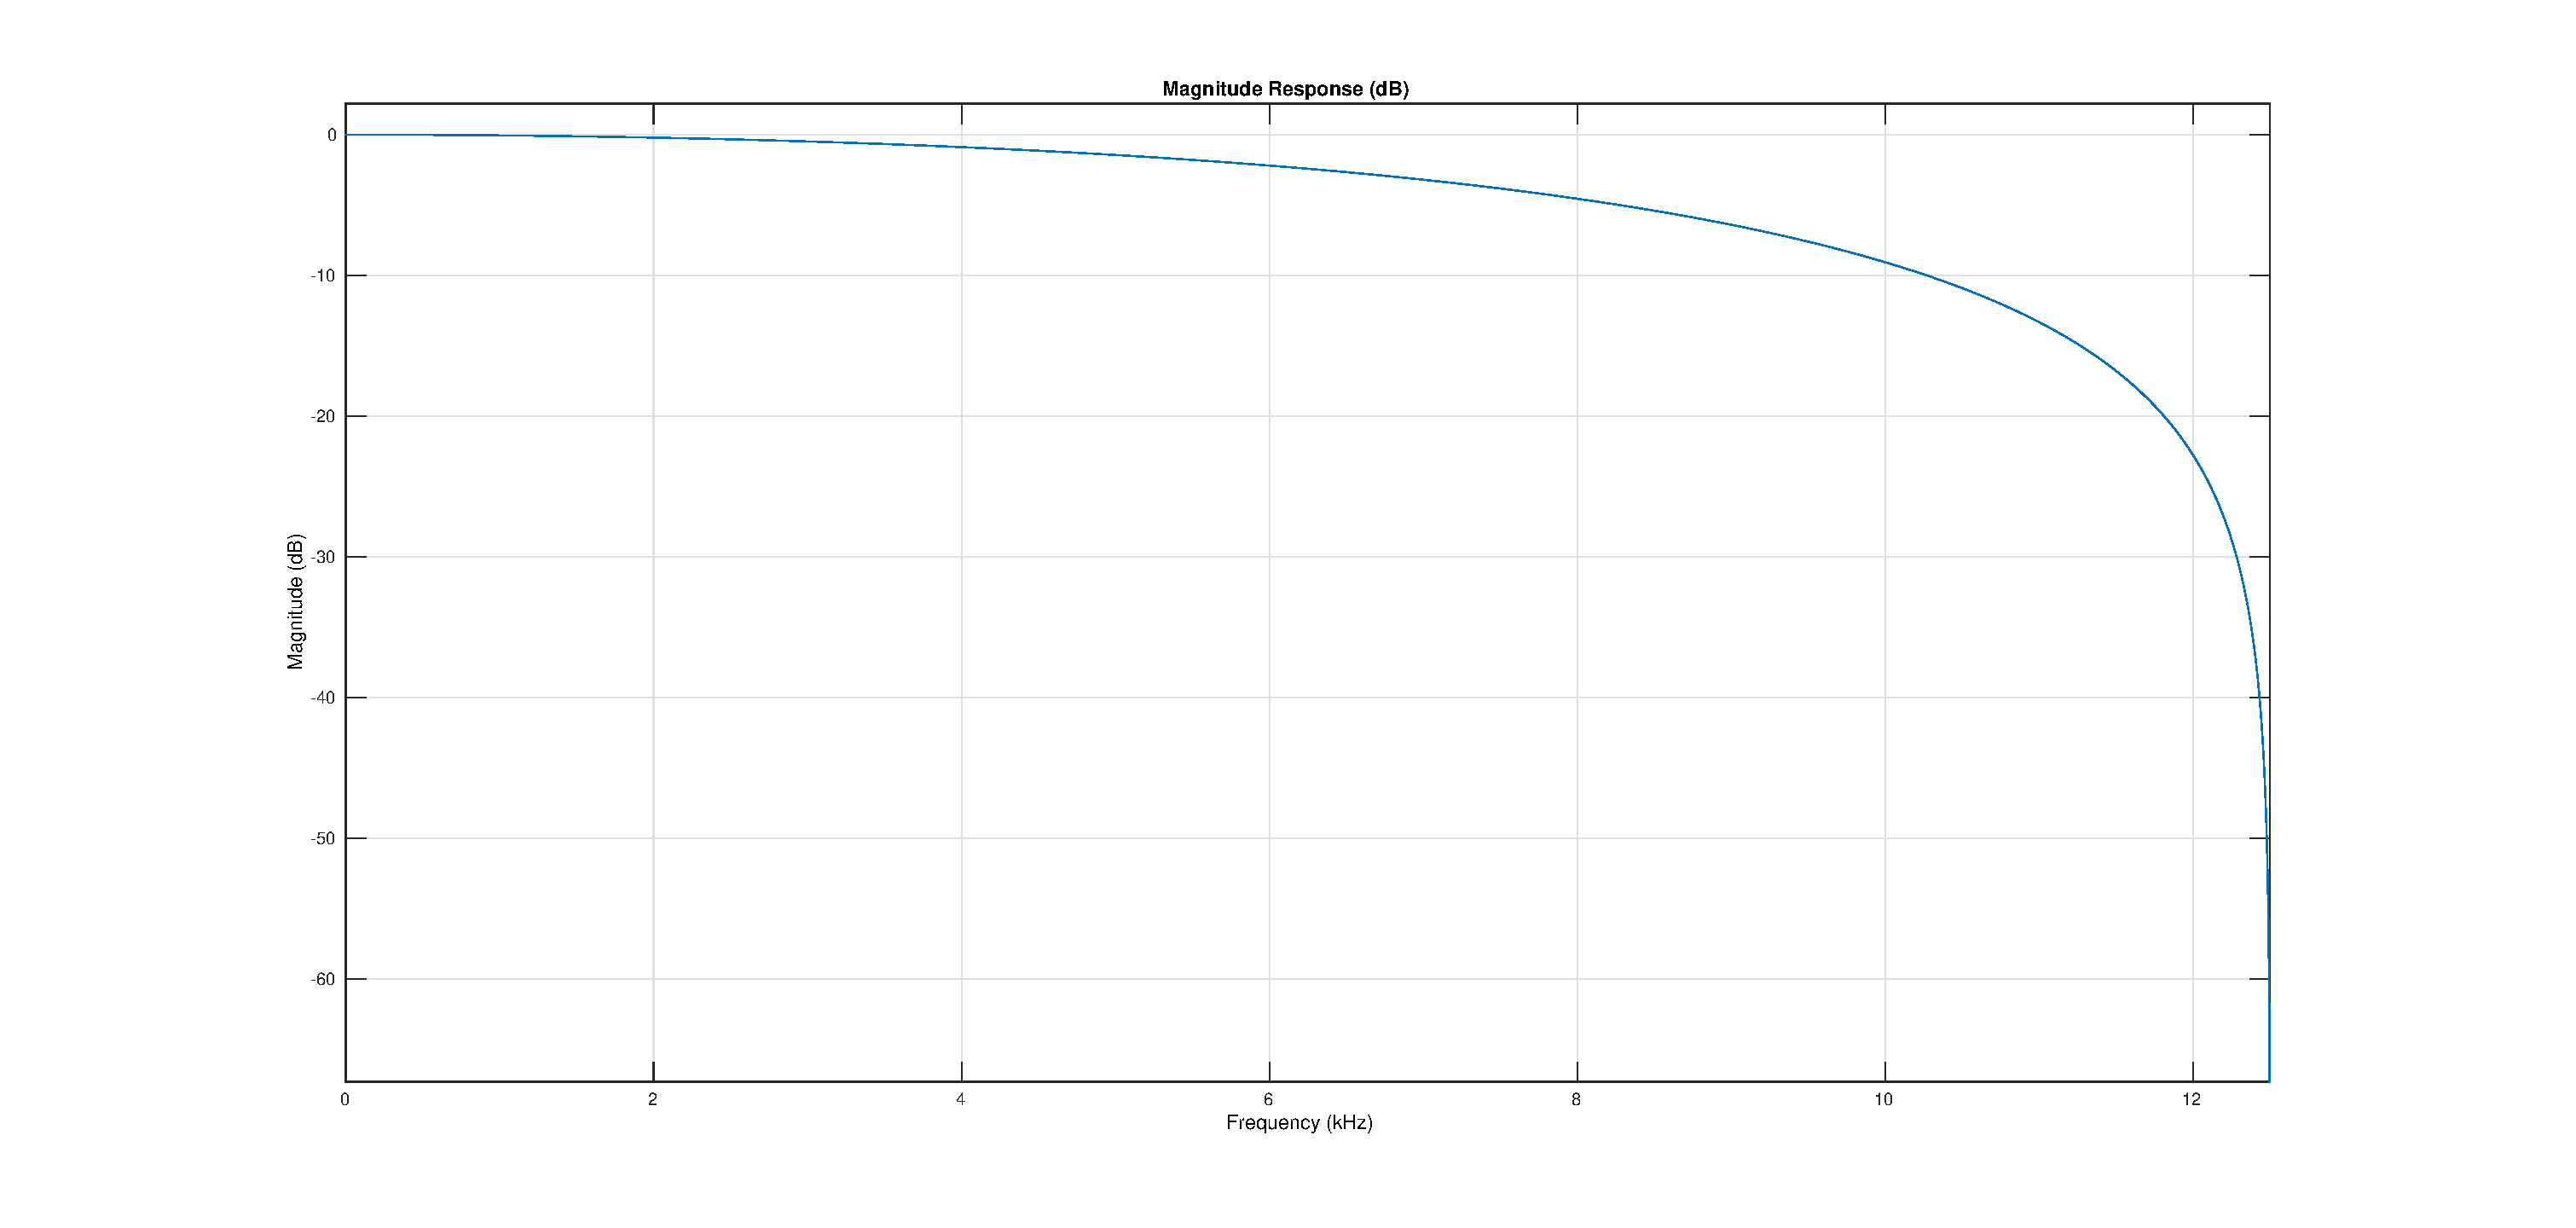
\includegraphics[width=6in]{images/frs/filter/rx/fmdemod_tau_mag.eps} \\
  \caption{Magnitude response of NBFM de-emphasis filter}
  \label{fig:deemph_iir}
\end{figure}

As of GNU Radio commit \texttt{ee369b92}, the \texttt{NBFM Receive} block also
performs a \ac{LPF} operation to limit the audio output.  The limit is hard coded
at 2.7 kHz with a 0.5 kHz transition band using a Hamming window.

Following the FM demodulation, the audio signal is routed to both a
\texttt{CTCSS Squelch} block and directly to a \texttt{Selector} block. When the
\ac{GUI} dropdown for the desired \ac{CTCSS} tone is set to ``None'' the
\texttt{Selector} passes the output of the \texttt{NBFM Receive} block to
the next stage. Otherwise, the \texttt{Selector} passes the output of the
\texttt{CTCSS Squelch} block, which is configured to pass samples when the
\ac{CTCSS} tone associated with the current \ac{GUI} dropdown widget selection
is detected.

Adequate values for the \texttt{CTCSS Squelch} values are determined
experimentally by interfacing with handheld \ac{FRS} radios, such as those
described in Section \ref{sec:testing}.
A \textit{Length} value of 6250 samples (250 ms at 25 kHz) and \textit{Level} of
0.010 are found to provide desirable squelch functionality.

\subsubsection{CTCSS Tone IIR Filter}

An astute listener can hear a number of the higher-frequency \ac{CTCSS} tones.
Therefore, a high-pass filter is needed to reject audio below 250.3 Hz. At a 25
kHz sample rate, an acceptable \ac{FIR} filter is found to require a large
number of taps \footnote{Approximately 900 taps for a FIR: Equiripple and 50dB of
stopband attenuation.}.  Instead, an \ac{IIR} filter is designed using \texttt{fdatool},
as this is expected to yield significantly fewer taps. The design parameters are
shown in Table \ref{tab:ctcss_filt}, and the filter response is presented in
Figure \ref{fig:ctcss_filt}.

\begin{table}[h]
  \centering
  \caption{Filter parameters of RX CTCSS-blocking high pass filter}
  \label{tab:ctcss_filt}
  \footnotesize
  \begin{tabular} {|l|l|}
    \hline
    \textbf{Design Method}                  & IIR: Elliptic         \\ \hline
    \textbf{Option: \textit{Match Exactly}} & both (pass and stop)  \\ \hline
    \textbf{Order}                          & 7                     \\ \hline
    \textbf{Sampling Frequency (kHz)}       & 25                    \\ \hline
    \textbf{Stopband Frequency (Hz)}        & 250.3                 \\ \hline
    \textbf{Passband Frequency (Hz)}        & 300                   \\ \hline
    \textbf{Passband Attenuation (dB)}      & 1                     \\ \hline
    \textbf{Stopband Attenuation (dB)}      & 50                    \\ \hline
  \end{tabular}
\end{table}

\begin{figure}[h!]
  \centering
  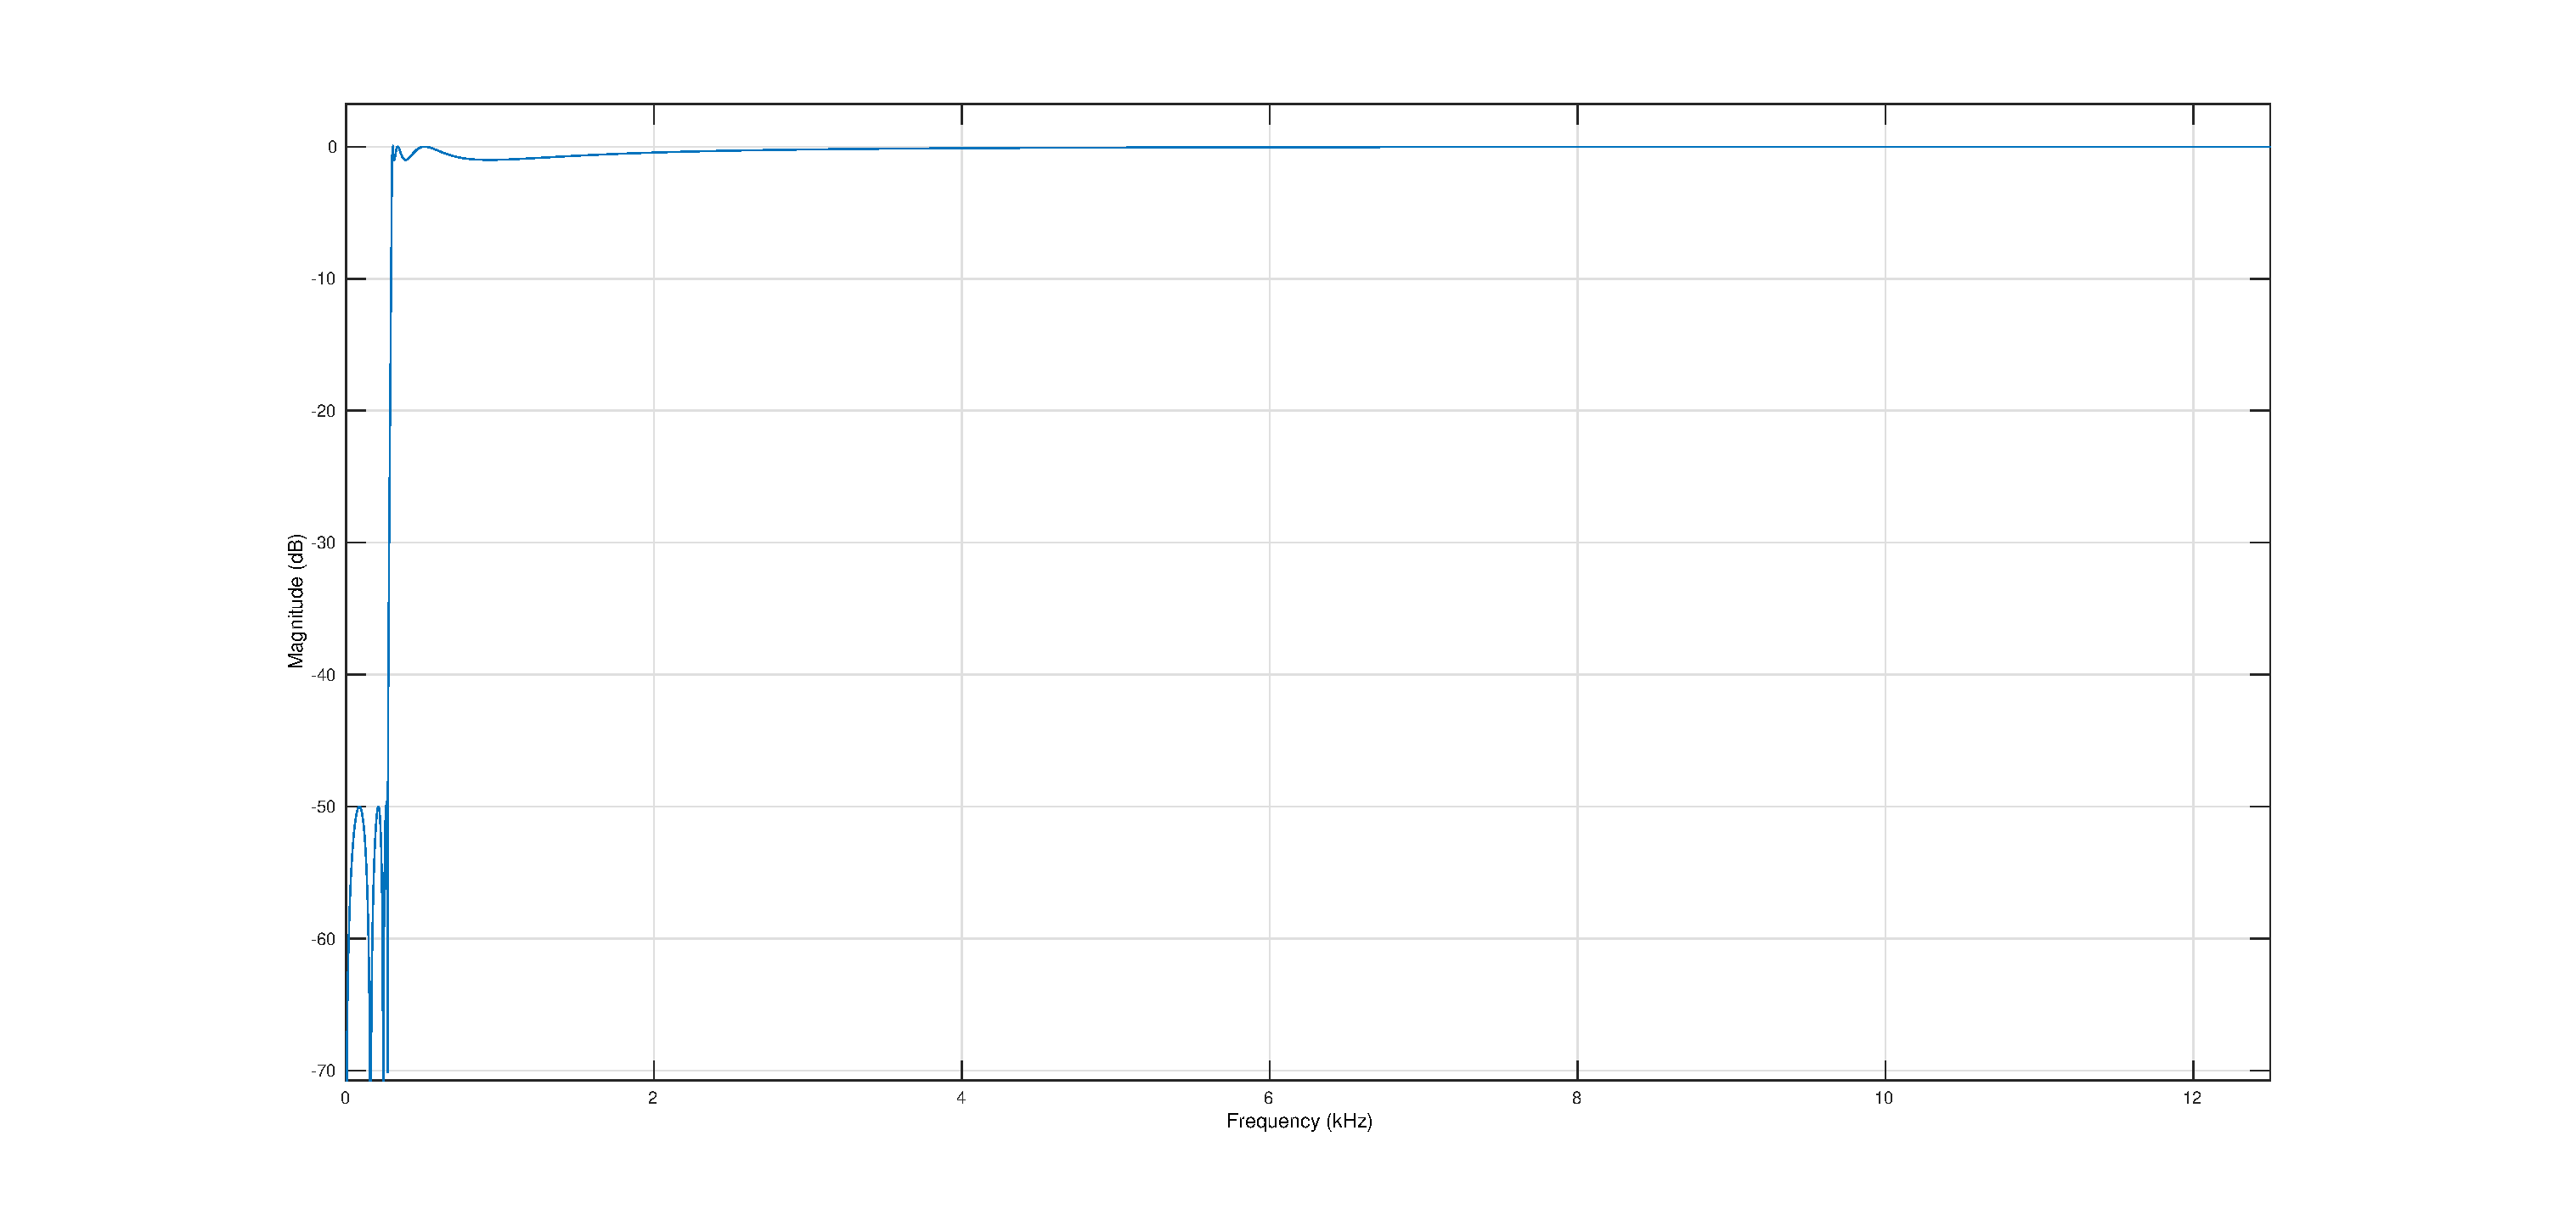
\includegraphics[width=6.5in]{images/frs/filter/rx/ctcss_hpf_mag.eps} \\
  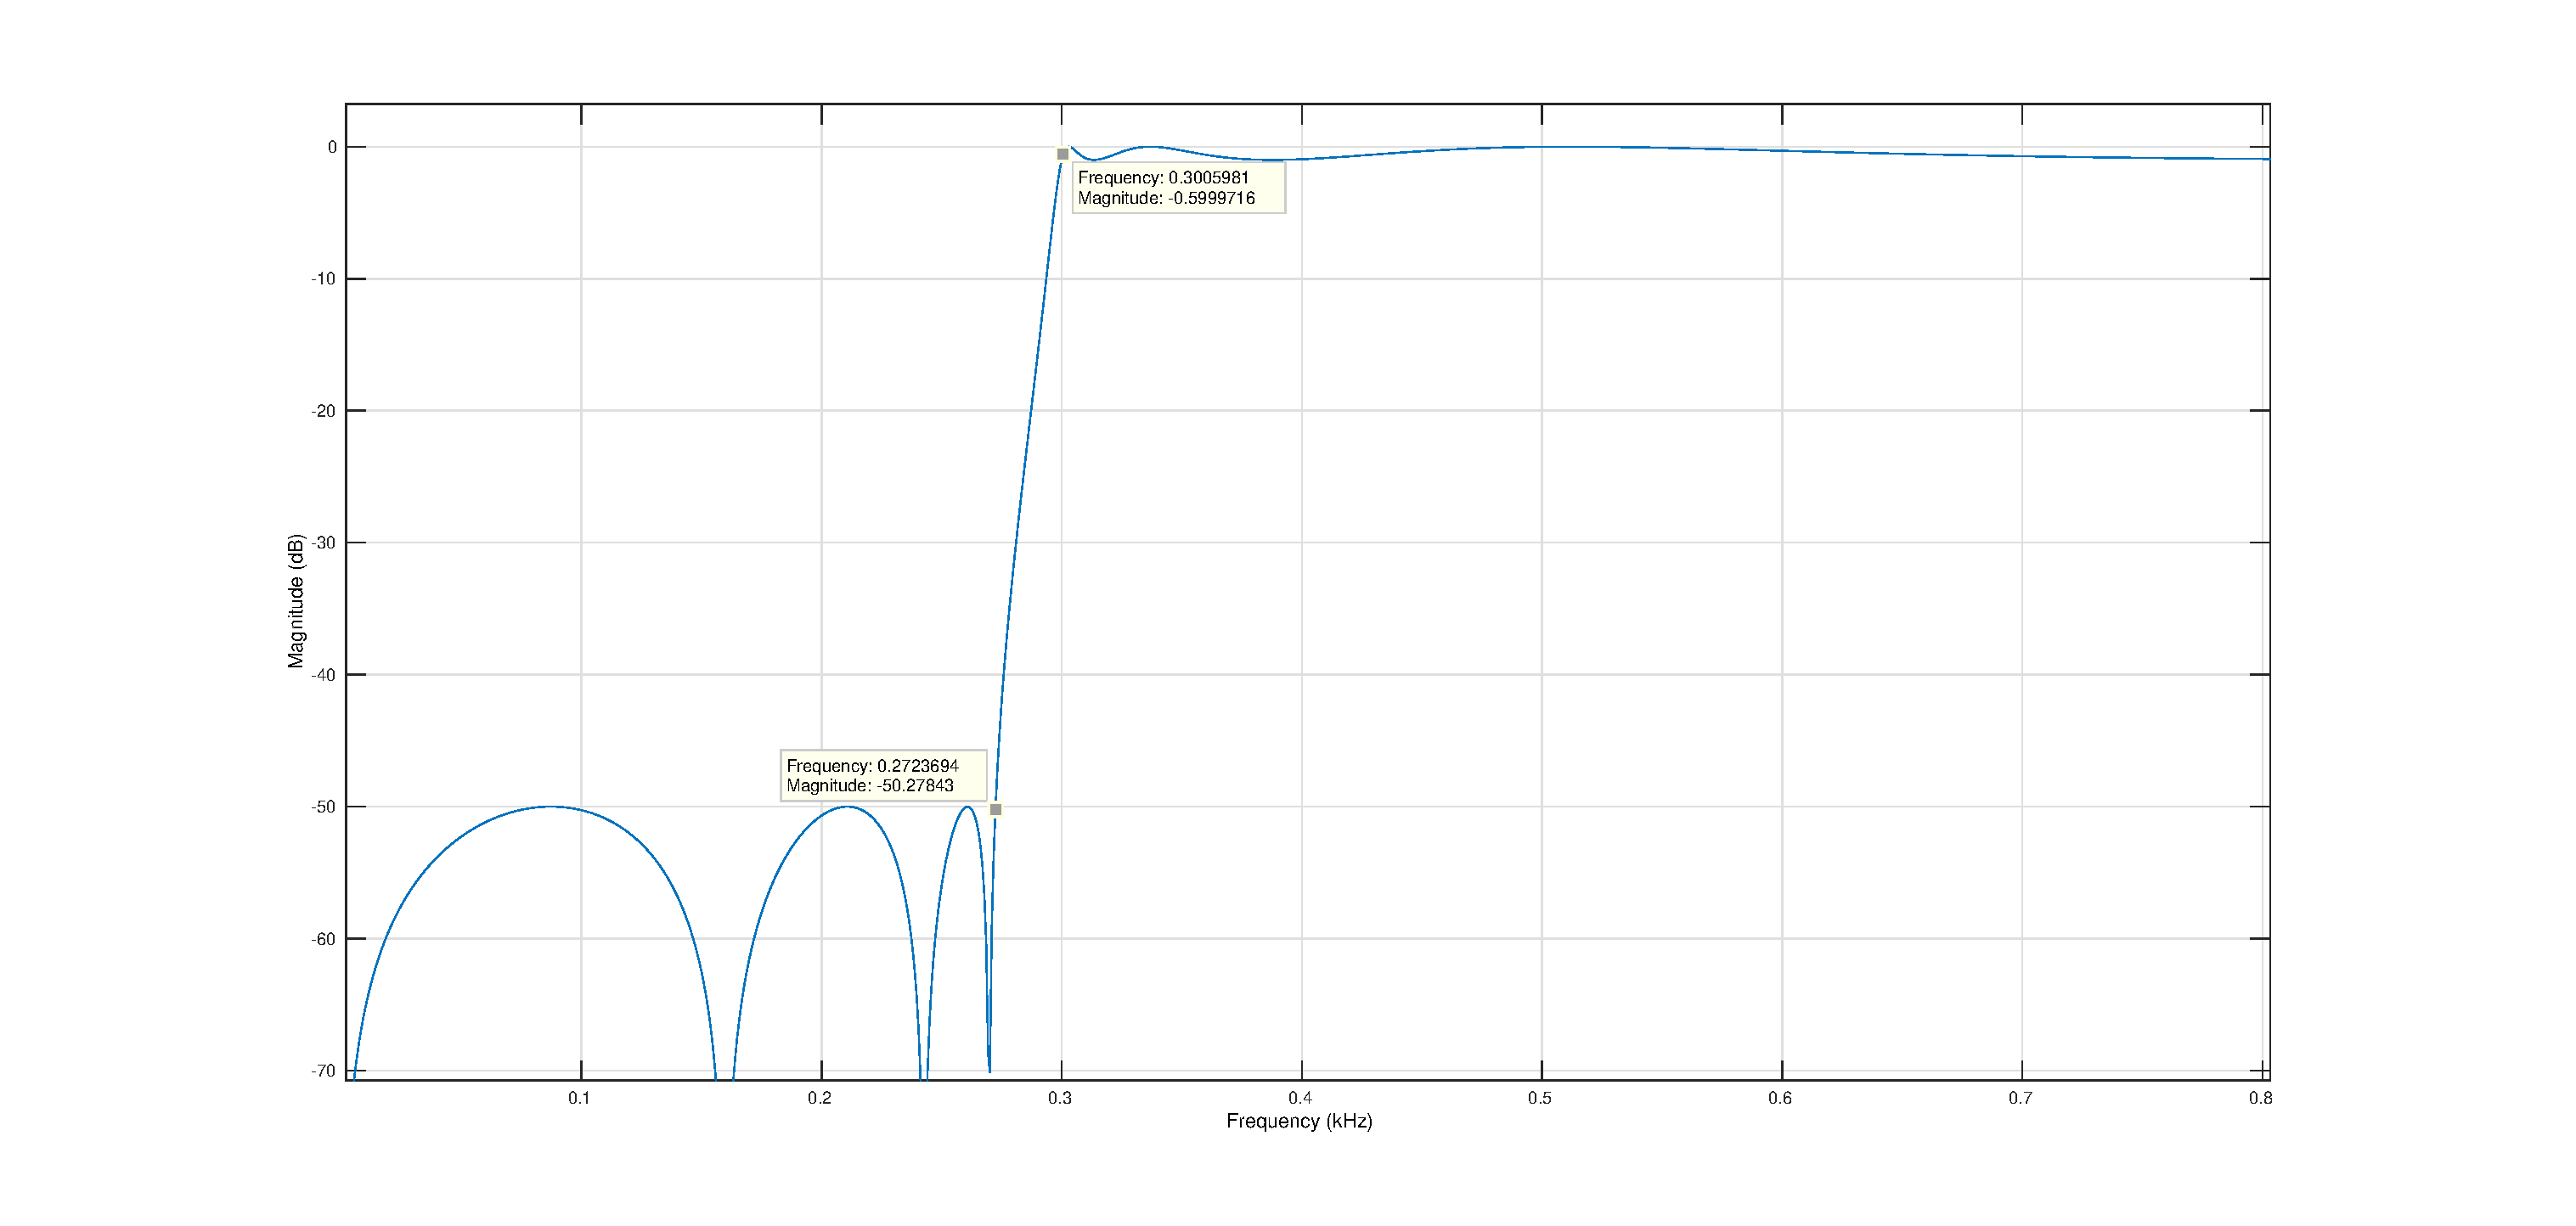
\includegraphics[width=6.5in]{images/frs/filter/rx/ctcss_hpf_mag_zoomed.eps} \\
  \caption{Response of RX CTCSS-blocking high pass filter}
  \label{fig:ctcss_filt}
\end{figure}

\subsubsection{Audio Sinks}
The audio from each \ac{FRS} channel is provided to
the system via the \texttt{Audio Sink} block. As done in the \ac{TX} path,
``pulse'' is specified for the \textit{Device Name} parameter to utilize the
PulseAudio subsystem. It is possible to use one sink per channel because the
underlying audio subsystem handles multiple inputs (from each sink). When
multiple channels are being received, all of them will be heard and combined
by the PulseAudio subsystem.

\cleardoublepage

\section{Testing and Evaluation} \label{sec:testing}

\subsection{Flowgraph GUI}
As noted in previous sections, various blocks provide \ac{GUI} widgets that may
be used to control and interact with the running flowgraph. Screen captures of
this \ac{GUI} are shown in Figures \ref{fig:gui_rx} and \ref{fig:gui_tx}.

The top of the \ac{GUI} provides quick access to \ac{CTCSS} tone selection and
the ability to enable/disable the \ac{RX} and \ac{TX} functionality.

By default, the \ac{CTCSS} dropdown is set to ``None.'' This can be changed at
any time, but it is recommended to make changes while \ac{RX} and \ac{TX} are
disabled, as portions of the flowgraph will be reconfigured.

The ``Enable RX'' checkbox is a master enable for all reception. Two master
enable options are provided for \ac{TX}. A ``Continuous Enable" checkbox enables
the \ac{TX} front end while the checkbox is marked. The ``Push to Talk'' button
enables the \ac{TX} front end only while this button is pressed.

The remainder of the \ac{GUI} is split between an \ac{RX} tab and a \ac{TX}
tab. Both views provide checkboxes for each \ac{FRS} channel. Marking the
checkbox enables reception/transmission of the associated channel. Gain controls
are also provided in each view.

The \ac{RX} view also provides control over the \texttt{Power Squelch} block
as the noise floor may vary in different environments.

Waterfall plots are provided for both groups of channels (1-7 and 8-14). These plots
display received signals in the frequency domain prior to any squelch blocks.
An ``Input Power'' meter is placed between these plots to provide a quick means
to determine if gains are set too high or too low.

The \ac{TX} side also provides waterfall plots. These are intended to provide
feedback in response to the user's checkbox selections.

\begin{figure}[H]
  \centering
  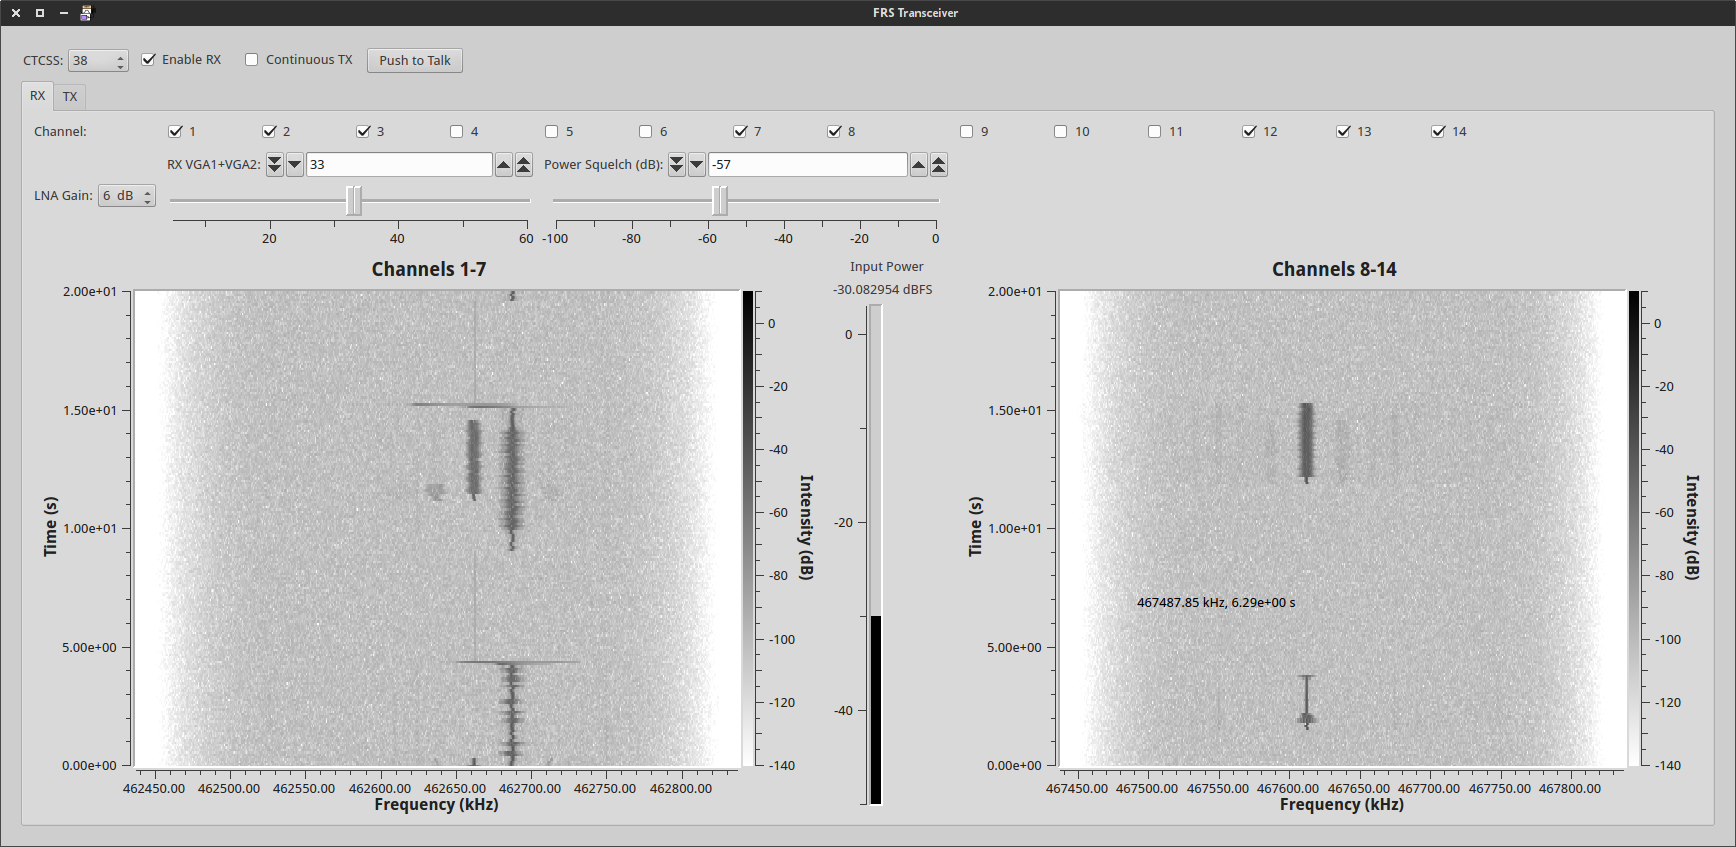
\includegraphics[width=6.5in]{images/frs/gui_rx.png}
  \caption{RX Section of the flowgraph GUI}
  \label{fig:gui_rx}
\end{figure}

\begin{figure}[H]
  \centering
  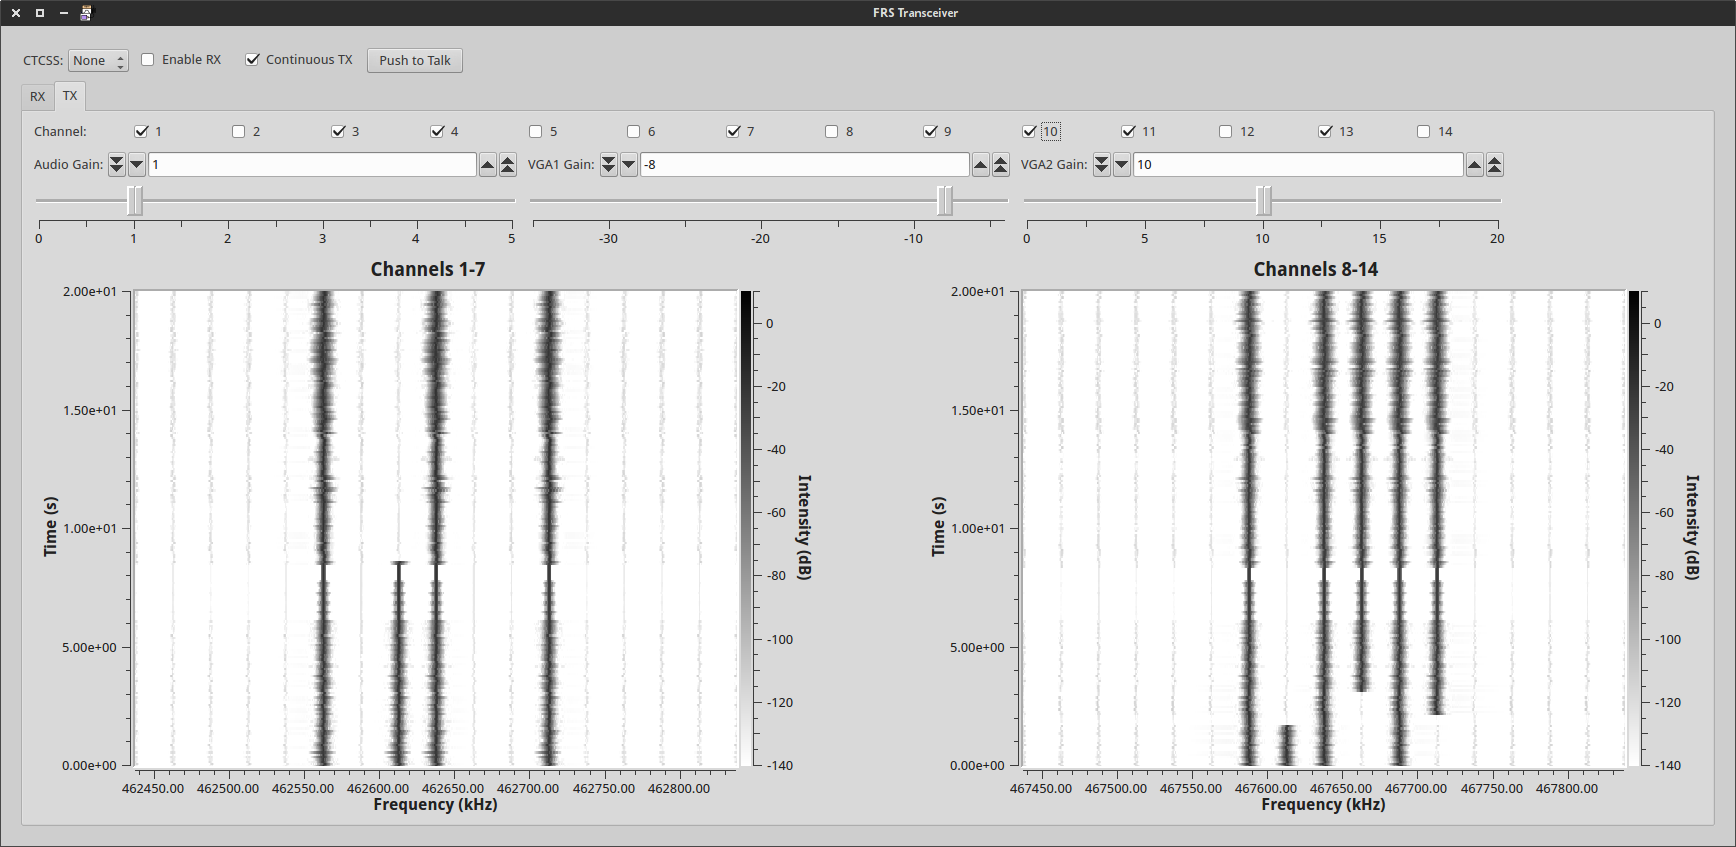
\includegraphics[width=6.5in]{images/frs/gui_tx.png}
  \caption{TX Section of the flowgraph GUI}
  \label{fig:gui_tx}
\end{figure}

\subsection{Nuand bladeRF SDR}
The Nuand bladeRF is a USB 3.0 \ac{SDR} with a frequency
range of 300~MHz to 3.8~GHz, full-duplex capabilities, a maximum bandwidth of
28~MHz, 12-bit samples, and a maximum sample rate of 40~MHz
\cite{BLADERF_BRIEF}. The architecture of the platform is illustrated in
Figure \ref{fig:bladerf_architecture}.

The bladeRF utilizes a Cypress FX3 USB3 device controller, which allows data to
be transferred between its USB 3.0 SuperSpeed connection and its parallel GPIF II
interface (running half-duplex at a speed of 100MHz). This is connected to an
Altera Cyclone IV E \ac{FPGA}. The \ac{FPGA} provides buffering and additional
signal processing, as well as control of the Lime Microsystems LMS6002D
Field-Programmable RF Transceiver.

The LMS6002D transceiver IC, whose architecture is depicted in in Figure
\ref{fig:lms6002d_architecture}, has multiple input and output RF ports
which are tuned to different frequency ranges.  The architecture is split into
a low band (300 MHz - 1500 MHz) and high band (1500 MHz - 3800 MHz). The LMS6002D contains
independently configurable RX and TX signal chains, which allows the bladeRF platform
to provide full-duplex capabilities. Also note that the RX and TX mixers each
have their own PLLs, which synthesize desired tuning frequencies from a
common input clock. These are what allow the device to operate the RX and TX
paths at different frequencies.

A single VCTCXO running at 38.4MHz supplies the FX3 and Silicon Labs Si5338
low-jitter clock generator.  All sample rate clocks are generated by the Si5338 with high
accuracy, allowing for flexible and arbitrary clocking of the ADC/DAC. The Si5338 also
supplies clocks to the Altera Cyclone \ac{FPGA} and to the Lime Microsystems LMS6002D.

\begin{figure}[H]
  \centering
  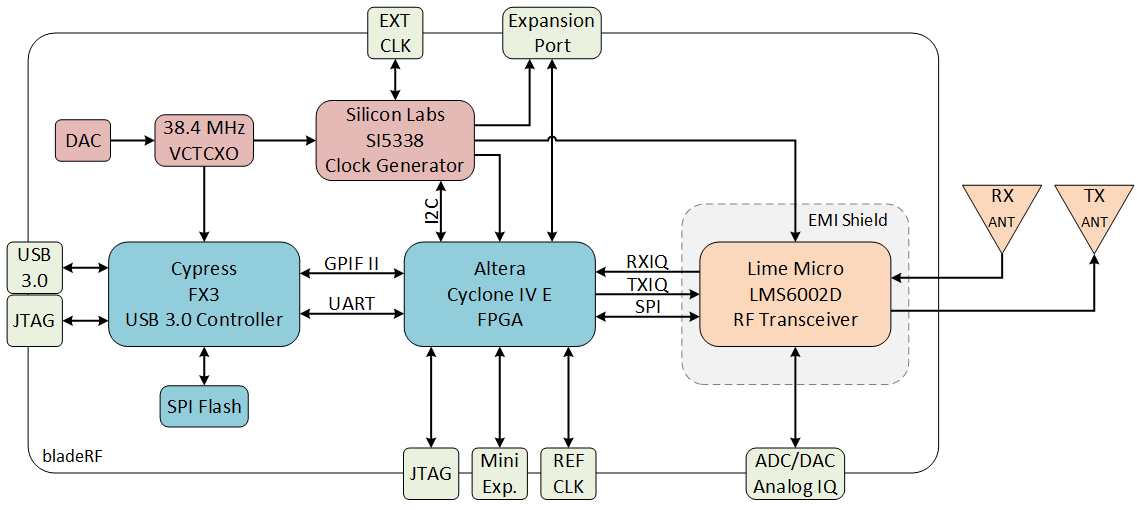
\includegraphics[width=6.5in]{images/bladerf_block_diagram.png}
  \caption{Nuand bladeRF architecture}
  \label{fig:bladerf_architecture}
\end{figure}

\begin{figure}[H]
  \centering
  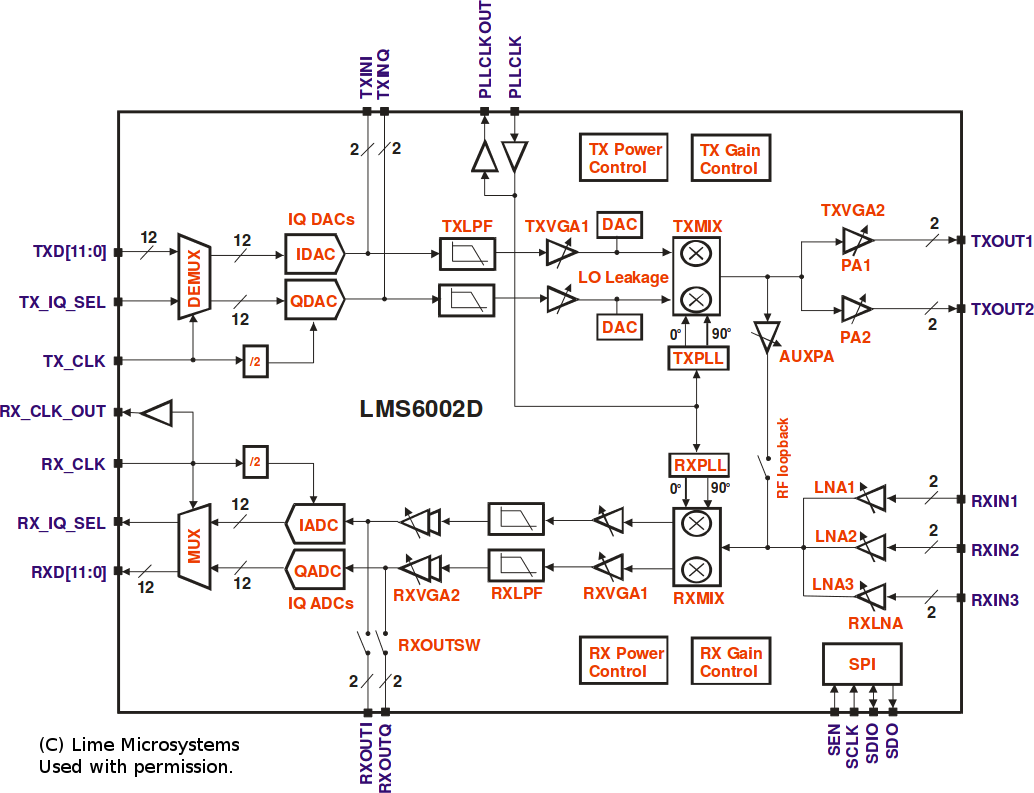
\includegraphics[width=5in]{images/lms6002d_block_diagram.png}
  \caption{Lime Microsystems LMS6002D architecture}
  \label{fig:lms6002d_architecture}
\end{figure}

\subsection{Reception}
To initially test reception, an Agilent E4433B signal generator \cite{SIGGEN}
is used to supply FM modulated tones to the bladeRF. This device is configured
to supply an FM-modulated 600 Hz tone with a deviation of 2.5 kHz and an
amplitude of -60 dBm.

The channel mapping is verified by supplying a signal at a specific \ac{FRS}
channel and checking that the demodulated signal is played only when that
associated channel is enabled in the \ac{GUI}. This is repeated for each of the 14
\ac{FRS} channels.

The per-channel filters are evaluated in a similar fashion, by verifying that
supplying a signal to the bladeRF on one channel does not yield significant
interference on neighboring channels.

Next, it is verified that none of the channels are attenuated significantly
more than others, as one might expect to occur if the decimating \ac{FIR}
filters had been designed to be too narrow. This is done by sweeping across
200 kHz of bandwidth with the signal generator, and noting the signal level
in the waterfall plots provided in the designed \ac{FRS} Transceiver \ac{GUI}. As
expected, attenuation begins occurring before channels 1 and 8, and after
channels 7 and 14. No significant attenuation is observed with the regions
containing the groups of 7 \ac{FRS} channels.

\begin{figure}[h]
  \centering
  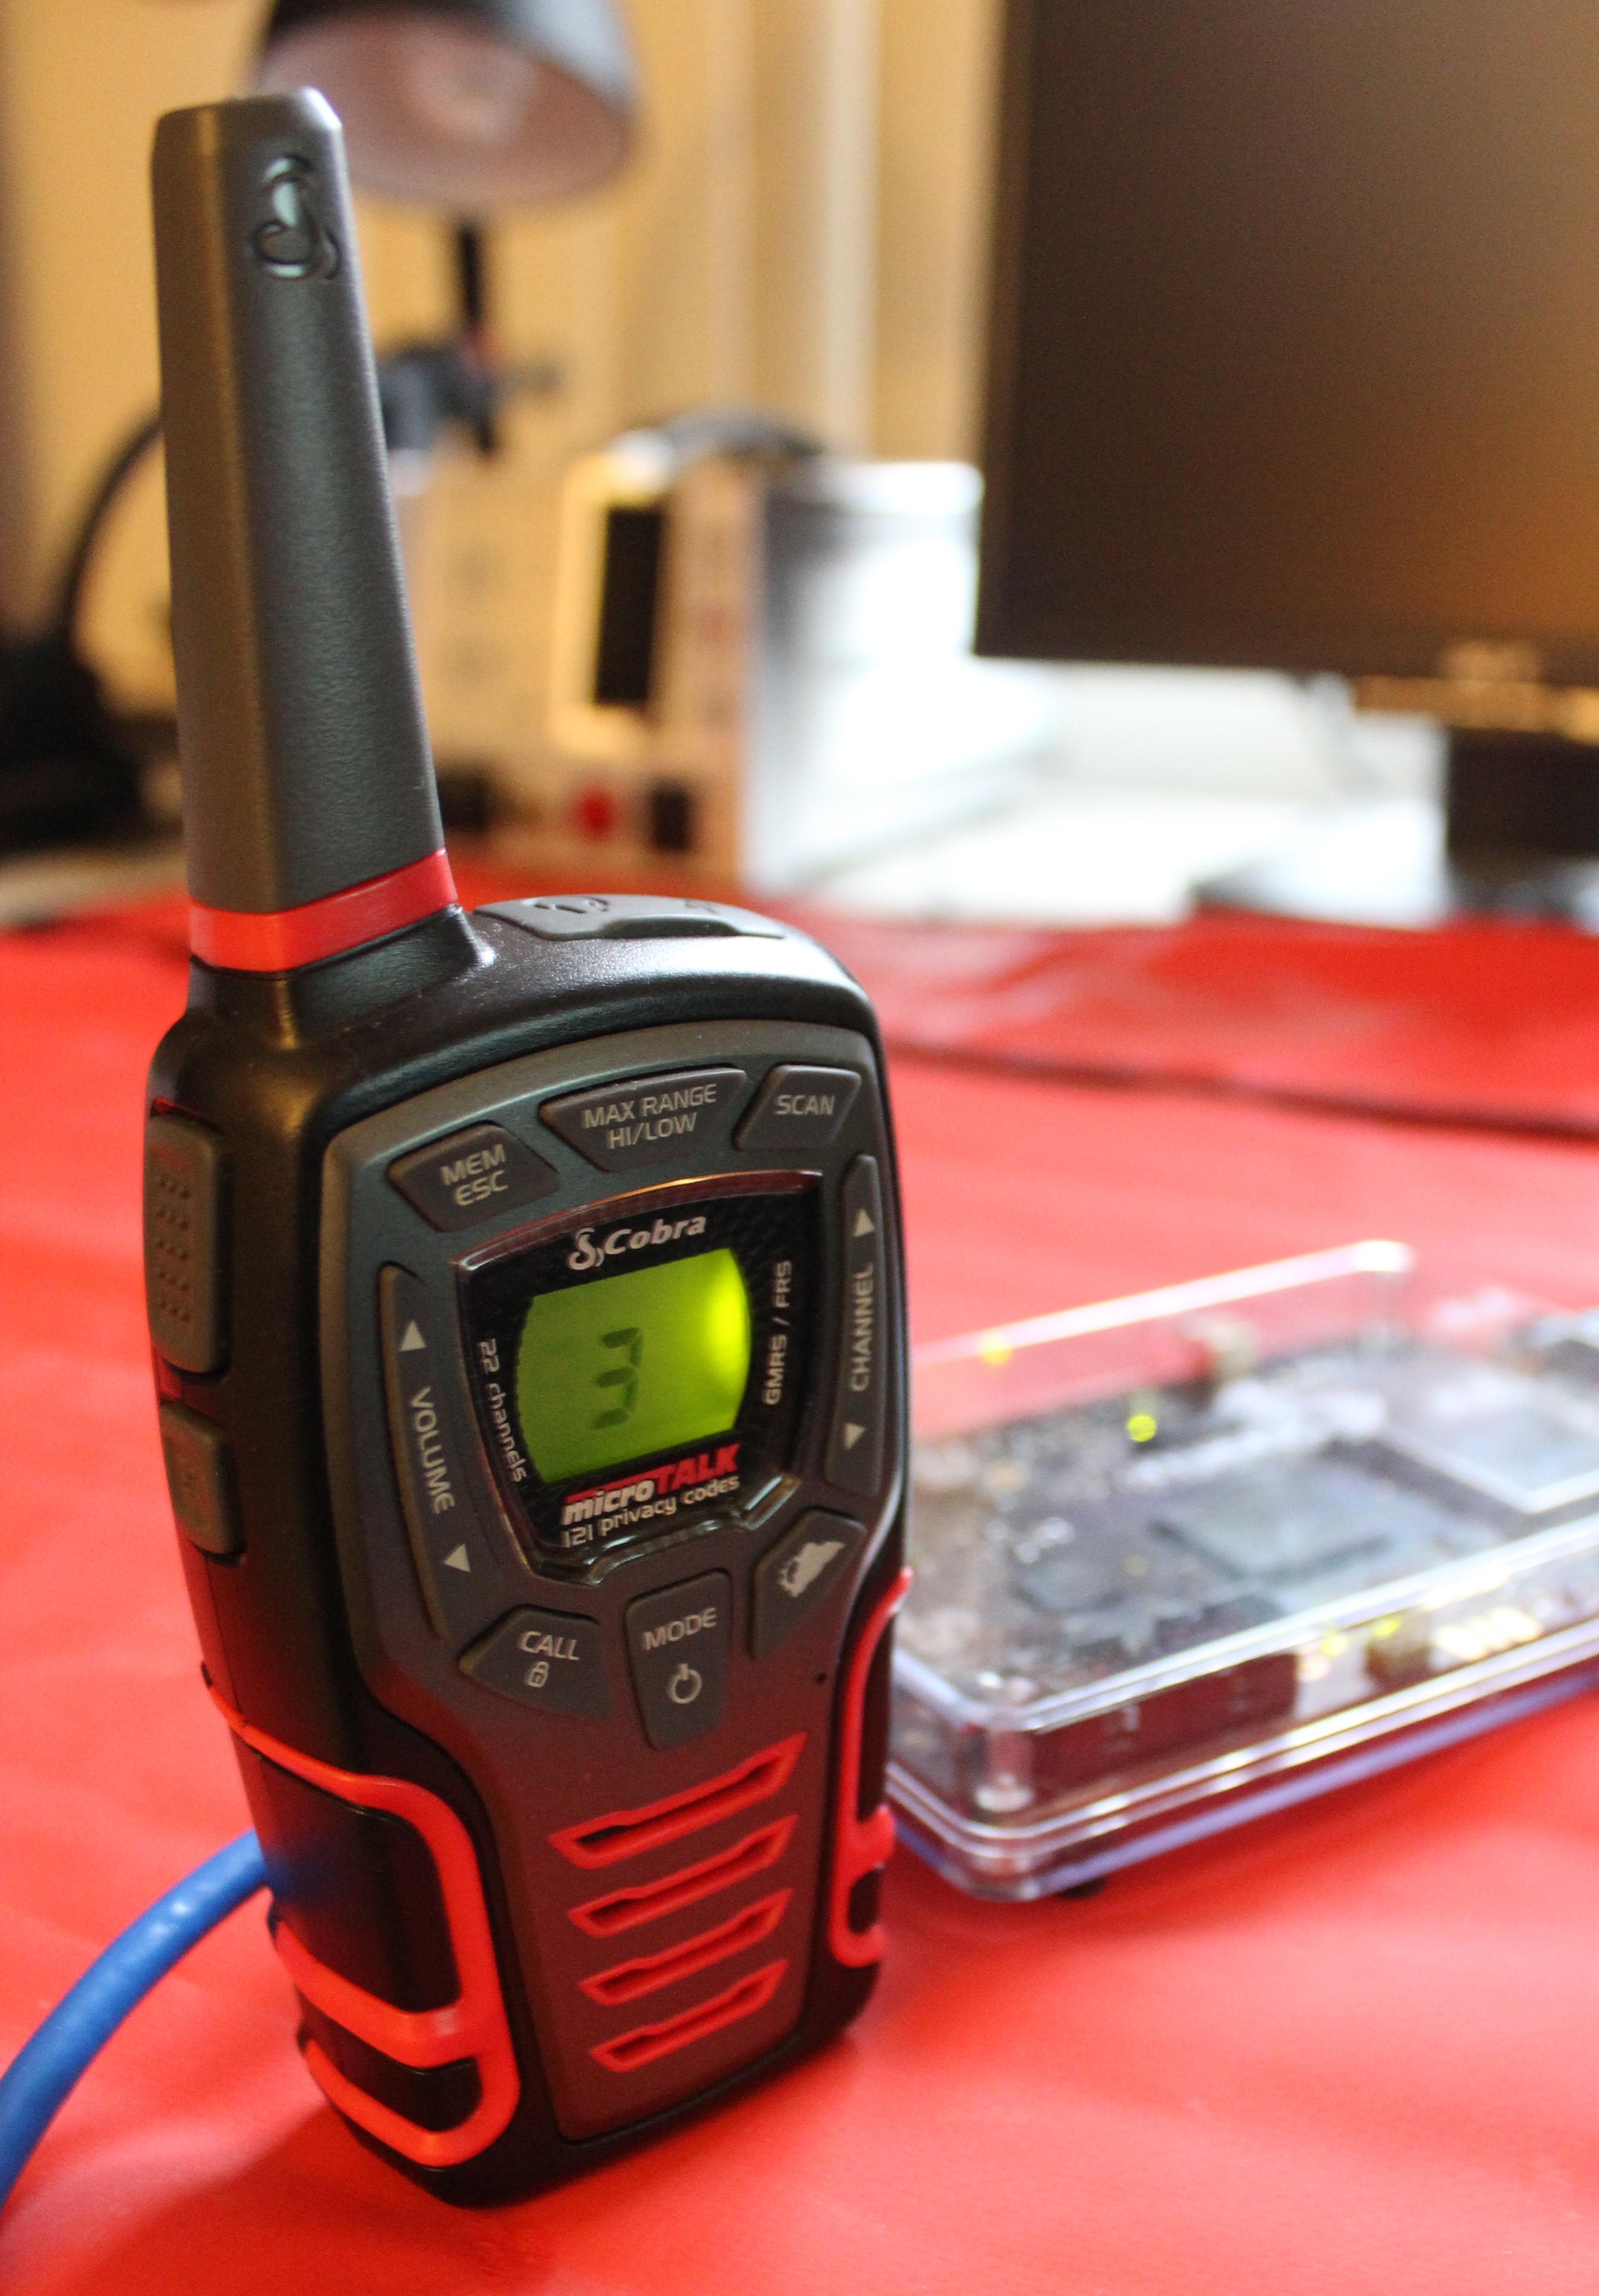
\includegraphics[width=2.5in]{images/frs/handheld.jpg}
  \caption{Cobra CXT545 FRS handheld transceiver used to test flowgraph}
  \label{fig:handheld}
\end{figure}

Next, interoperability with commercially-available handheld \ac{FRS}
transceivers is tested. A pair of Cobra CXT545 \cite{COBRA_CXT545} walkie
talkies, configured for low power operation on FRS channels (Figure
\ref{fig:handheld}) are used.  These devices support all 38 of the commonly used
\ac{CTCSS} tones listed in Table \ref{tab:ctcss}, with 67.0 Hz being \ac{CTCSS}
tone \#1, and 250.3 Hz being tone \#38.

Within the confines of a lab environment, the output power of these radios
is found to saturate the bladeRF input. This is addressed by reducing the
gain values used for reception and/or using external attenuators.

The channel mapping and per-channel filter tests are performed again using
these devices. The \ac{CTCSS} squelch functionality is verified by transmitting
with each tone on the handheld, and confirming that the audio is played by the
flowgraph only when ``None'' or the associated \ac{CTCSS} tone is selected in
the \ac{GUI}.

\subsection{Transmission}

The waterfall plots in the \ac{TX} portion of the flowgraph are used to provide
confirmation that each channel's signal is located at the correct offset.
To further evaluate the signal being supplied to the bladeRF for transmission, a
\texttt{Qt GUI Frequency Sink} is connected in parallel to the
\texttt{osmocom Sink} block. For a higher-resolution view of a group of channels,
a frequency sink block is placed in parallel with the first
\texttt{Interpolating FIR Filter} block.

Figure \ref{fig:osmo-ch8-14} depicts the digital representation of the signal
containing a concurrent transmission on channels 8 through 14 while Figure
\ref{fig:osmo-ch8} show a transmission containing only channel 8. A plot
containing the simultaneous transmission on all 14 channels is presented in
Figure \ref{fig:osmo-all}.

\begin{figure}[H]
  \centering
  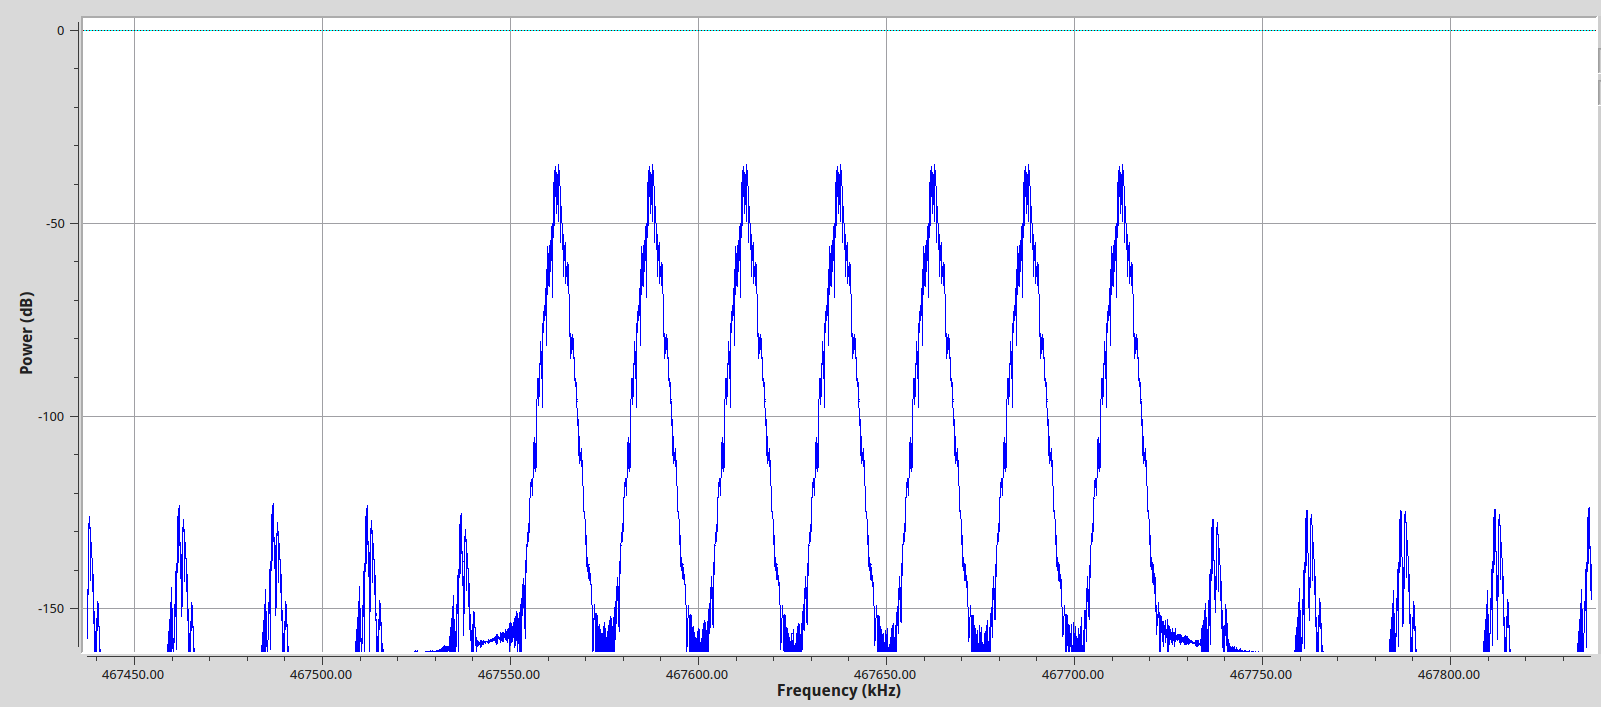
\includegraphics[width=4.75in]{images/frs/results/osmo-ch8-14.png}
  \caption{FFT plot of digital signal containing FRS channels 8-14}
  \label{fig:osmo-ch8-14}
\end{figure}

\begin{figure}[H]
  \centering
  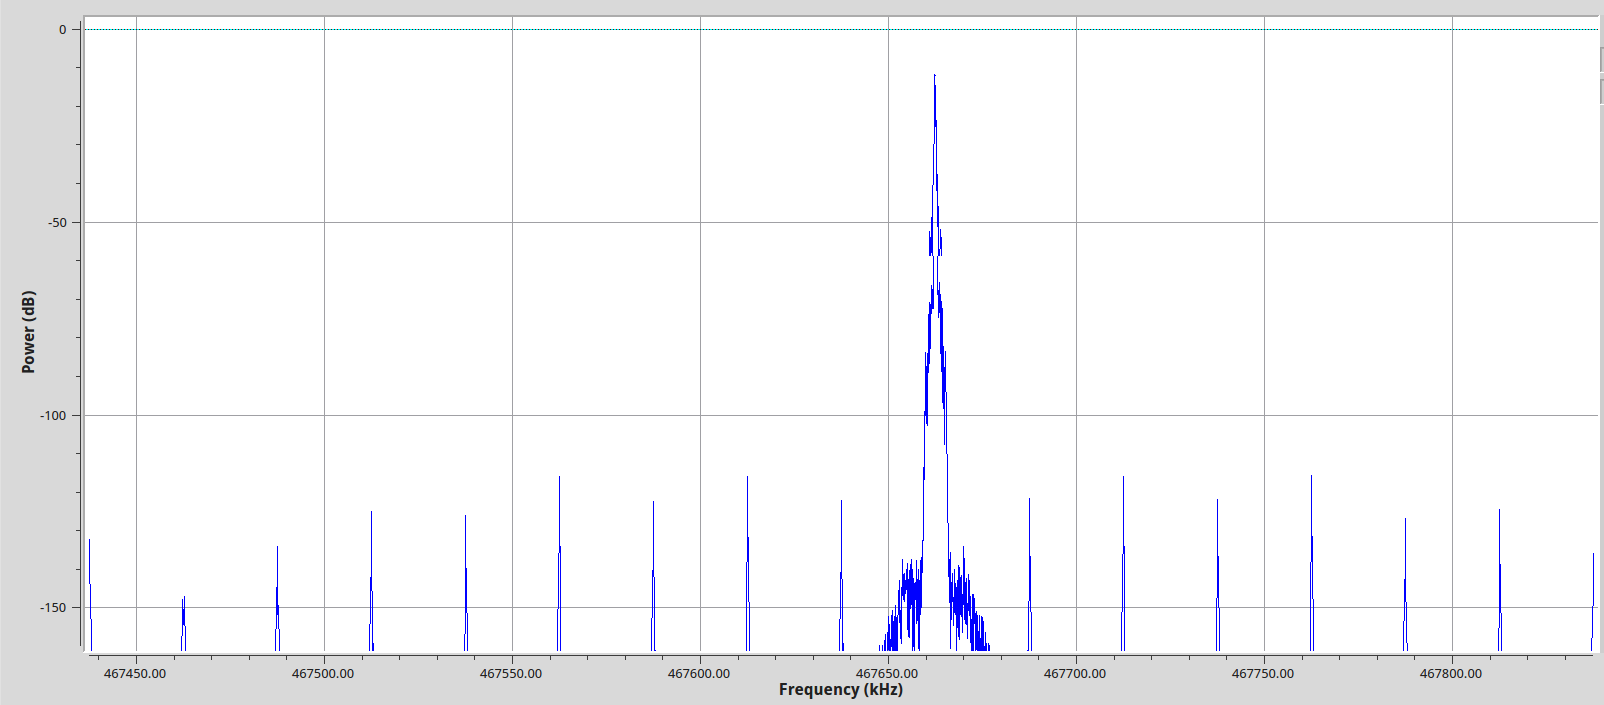
\includegraphics[width=4.75in]{images/frs/results/osmo-ch8.png}
  \caption{FFT plot of digital signal containing FRS channel 8}
  \label{fig:osmo-ch8}
\end{figure}

\begin{figure}[H]
  \centering
  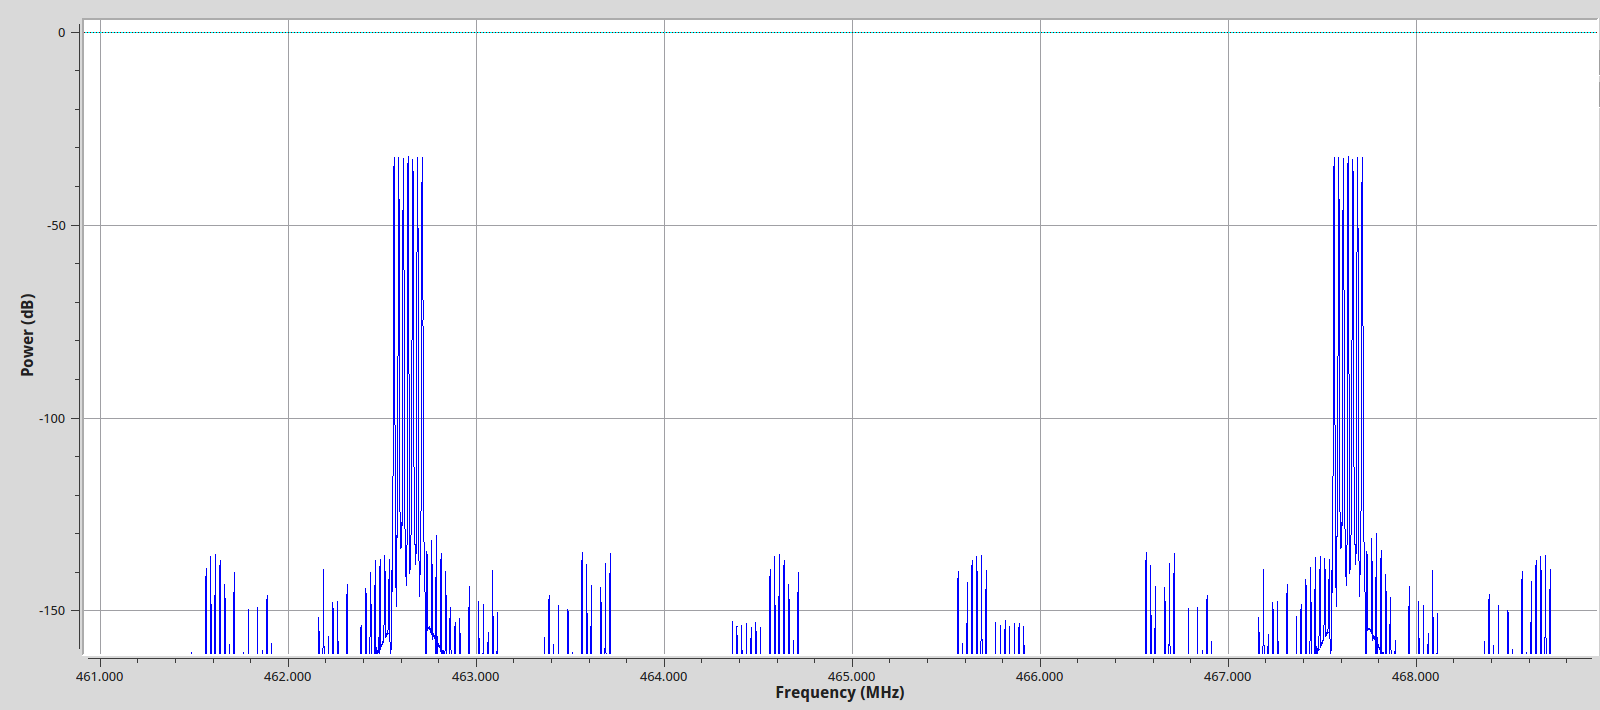
\includegraphics[width=4.75in]{images/frs/results/osmo_all_ch.png}
  \caption{FFT plot of digital signal containing all FRS channels}
  \label{fig:osmo-all}
\end{figure}

Per these plots, the channels are located at the expected frequencies, with
bandwidths within the 12.kHz maximum. The expected aliases that occur as a side
effect of polyphase synthesis \cite{TRONDEAU_PFB} are significantly rejected by
the designed filters and are observed to occur 100 dB below the signals of
interest.

Next, the output of the bladeRF's \ac{TX} port is observed, using an
Agilent E4406A \ac{VSA} \cite{VSA}. Again, the locations and widths channels
are first verified to be correct.

The signal levels of the \ac{FRS} signals and the expected aliases are found to
be within acceptable limits. It is noted that the magnitudes do differ from the
digital representation to some degree. This may be attributed to quantization
error that is inherent in converting a digital floating point signal to an
analog signal through the hardware's 12-bit \ac{DAC}. This can be simulated in
\ac{GRC} by adding a \texttt{Quantizer} block (found under ``Impairment
Models'') prior to the \texttt{osmocom Sink} block.

As discussed in Section \ref{sec:design}, the bladeRF's \ac{TX} frequency
is tuned 200 kHz under 465.1375 MHz -- the frequency that is equidistant from both
groups of channels -- to avoid distortion caused by any IQ imbalance.

The effectiveness of this strategy is made clear by Figure \ref{fig:vsa-all}.
Note that to the left of each group of \ac{FRS} signals, a significantly
attenuated image from the other group is present. By ensuring these images
do not overlap with the intended signal, a higher \ac{SINAD} is achieved.

\begin{figure}[h]
  \centering
  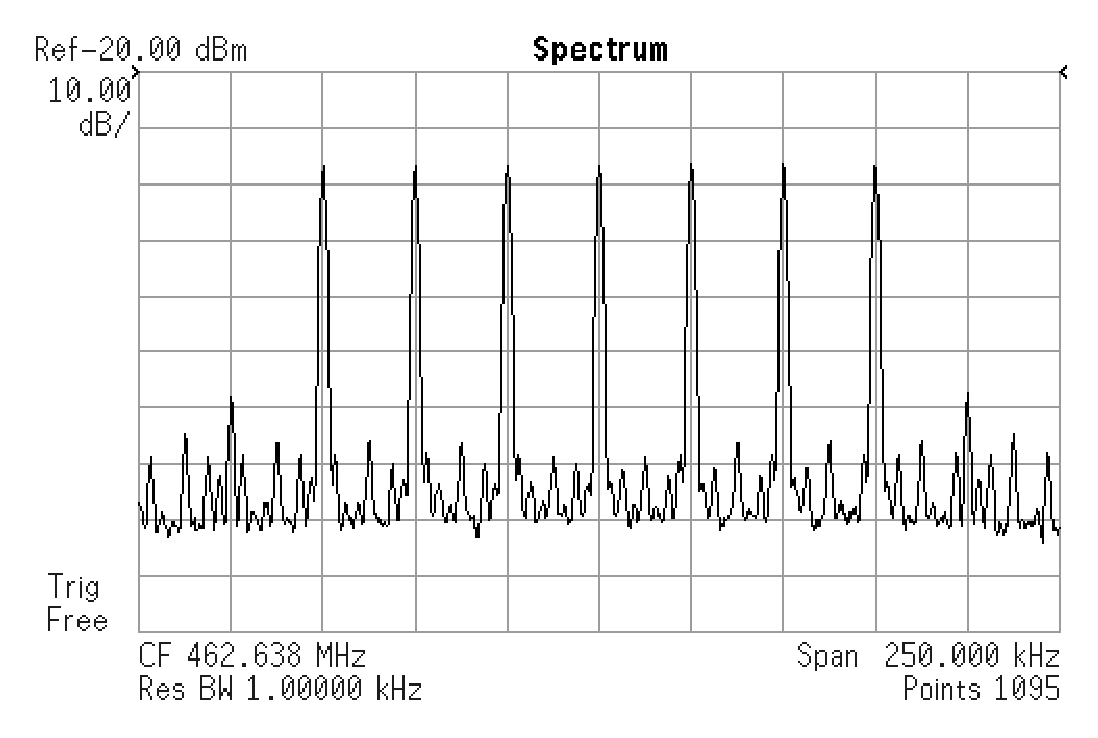
\includegraphics[width=3.5in]{images/frs/results/ch1-7.eps}
  \caption{FFT plot of analog signal containing FRS channels 1-7}
  \label{fig:vsa-ch1-7}
\end{figure}

\begin{figure}[h]
  \centering
  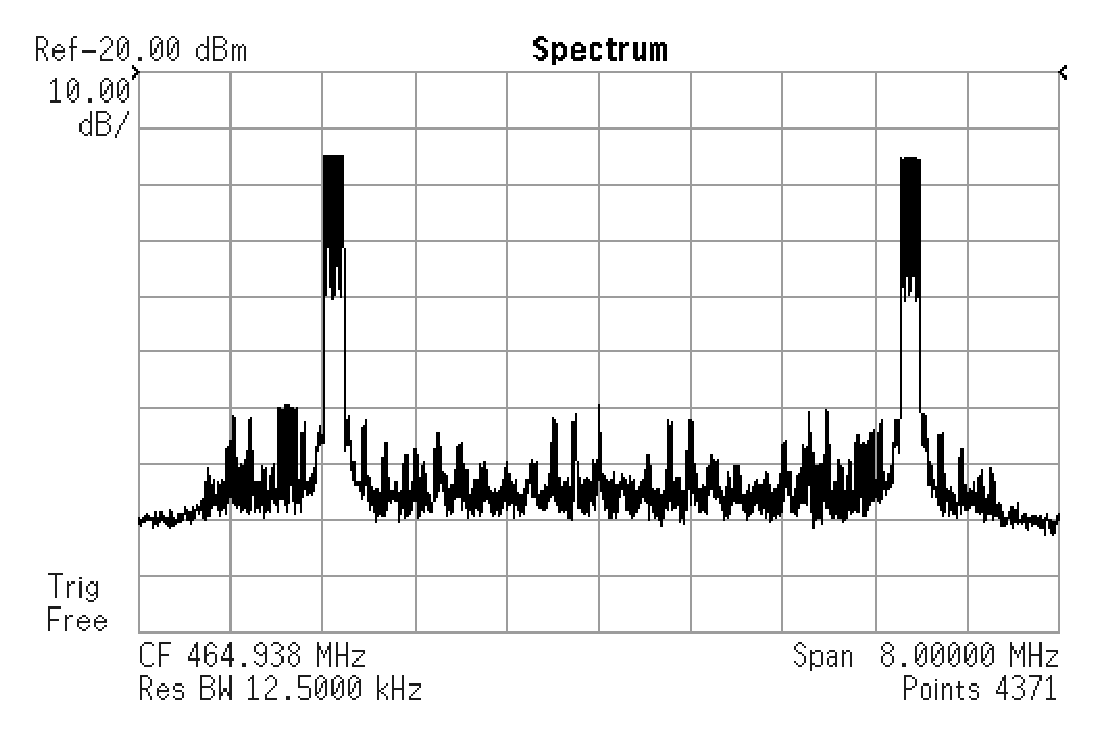
\includegraphics[width=3.5in]{images/frs/results/all_ch_enabled.eps}
  \caption{FFT plot of analog signal containing all 14 FRS channels}
  \label{fig:vsa-all}
\end{figure}

\newpage
\section{Software and System Configuration} \label{sec:sys_config}

The design and evaluation of the flowgraph described in this document is
performed with XUbuntu 14.10 \cite{XUBUNTU}, on machines with Intel i7
processors, more than 4 GB of RAM, and either Intel XHCI 7 Series or Renesas
uPD720202 USB 3.0 host controllers. Similar or better systems are recommended.

Due to the sample rates used in this flowgraph, USB 3.0 is required for
full-duplex operation. Be aware that even for half-duplex operation, USB 2.0
controllers may not be able to support the required 32 MB/s\footnote{Although
the theoretical max throughput of USB 2.0 is 60 MB/s, the practical achievable
throughput is significantly less due to protocol overheads.}

Table \ref{tab:versions} lists the minimum required software versions needed to
use this transceiver. Newer versions of the listed items should also be
compatible.

\begin{table}[h]
  \centering
  \caption{Minimum required component versions}
  \label{tab:versions}
  \footnotesize
  \begin{tabular} {|l|l|}
    \hline
    \textbf{Component}                   & \textbf{Version} \\ \hline
    \hline
    \textbf{bladeRF FPGA}               & 0.1.2             \\ \hline
    \textbf{bladeRF Firmware}           & 1.8.0             \\ \hline
    \textbf{libbladeRF}                 & 1.2.1             \\ \hline
    \textbf{GNU Radio}                  & 3.7.7             \\ \hline
    \textbf{gr-osmosdr}                 & 0.1.4-g48045b59   \\ \hline
  \end{tabular}
\end{table}

The ``Getting Started'' guide on the bladeRF wiki
\cite{BLADERF_GETTING_STARTED} provides instructions for installing the latest
versions of the above items. Those new to the bladeRF and GNU Radio may wish to
use the GNU Radio Live SDR Environment \cite{GNU_RADIO_LIVE_IMAGE} , an
Ubuntu-based live image with GNU Radio and SDR support pre-installed.

\newpage
\section{Flowgraph Diagrams} \label{sec:diagrams}
\begin{figure}[h!]
  \label{fig:full_flowgraph}
  \centering
  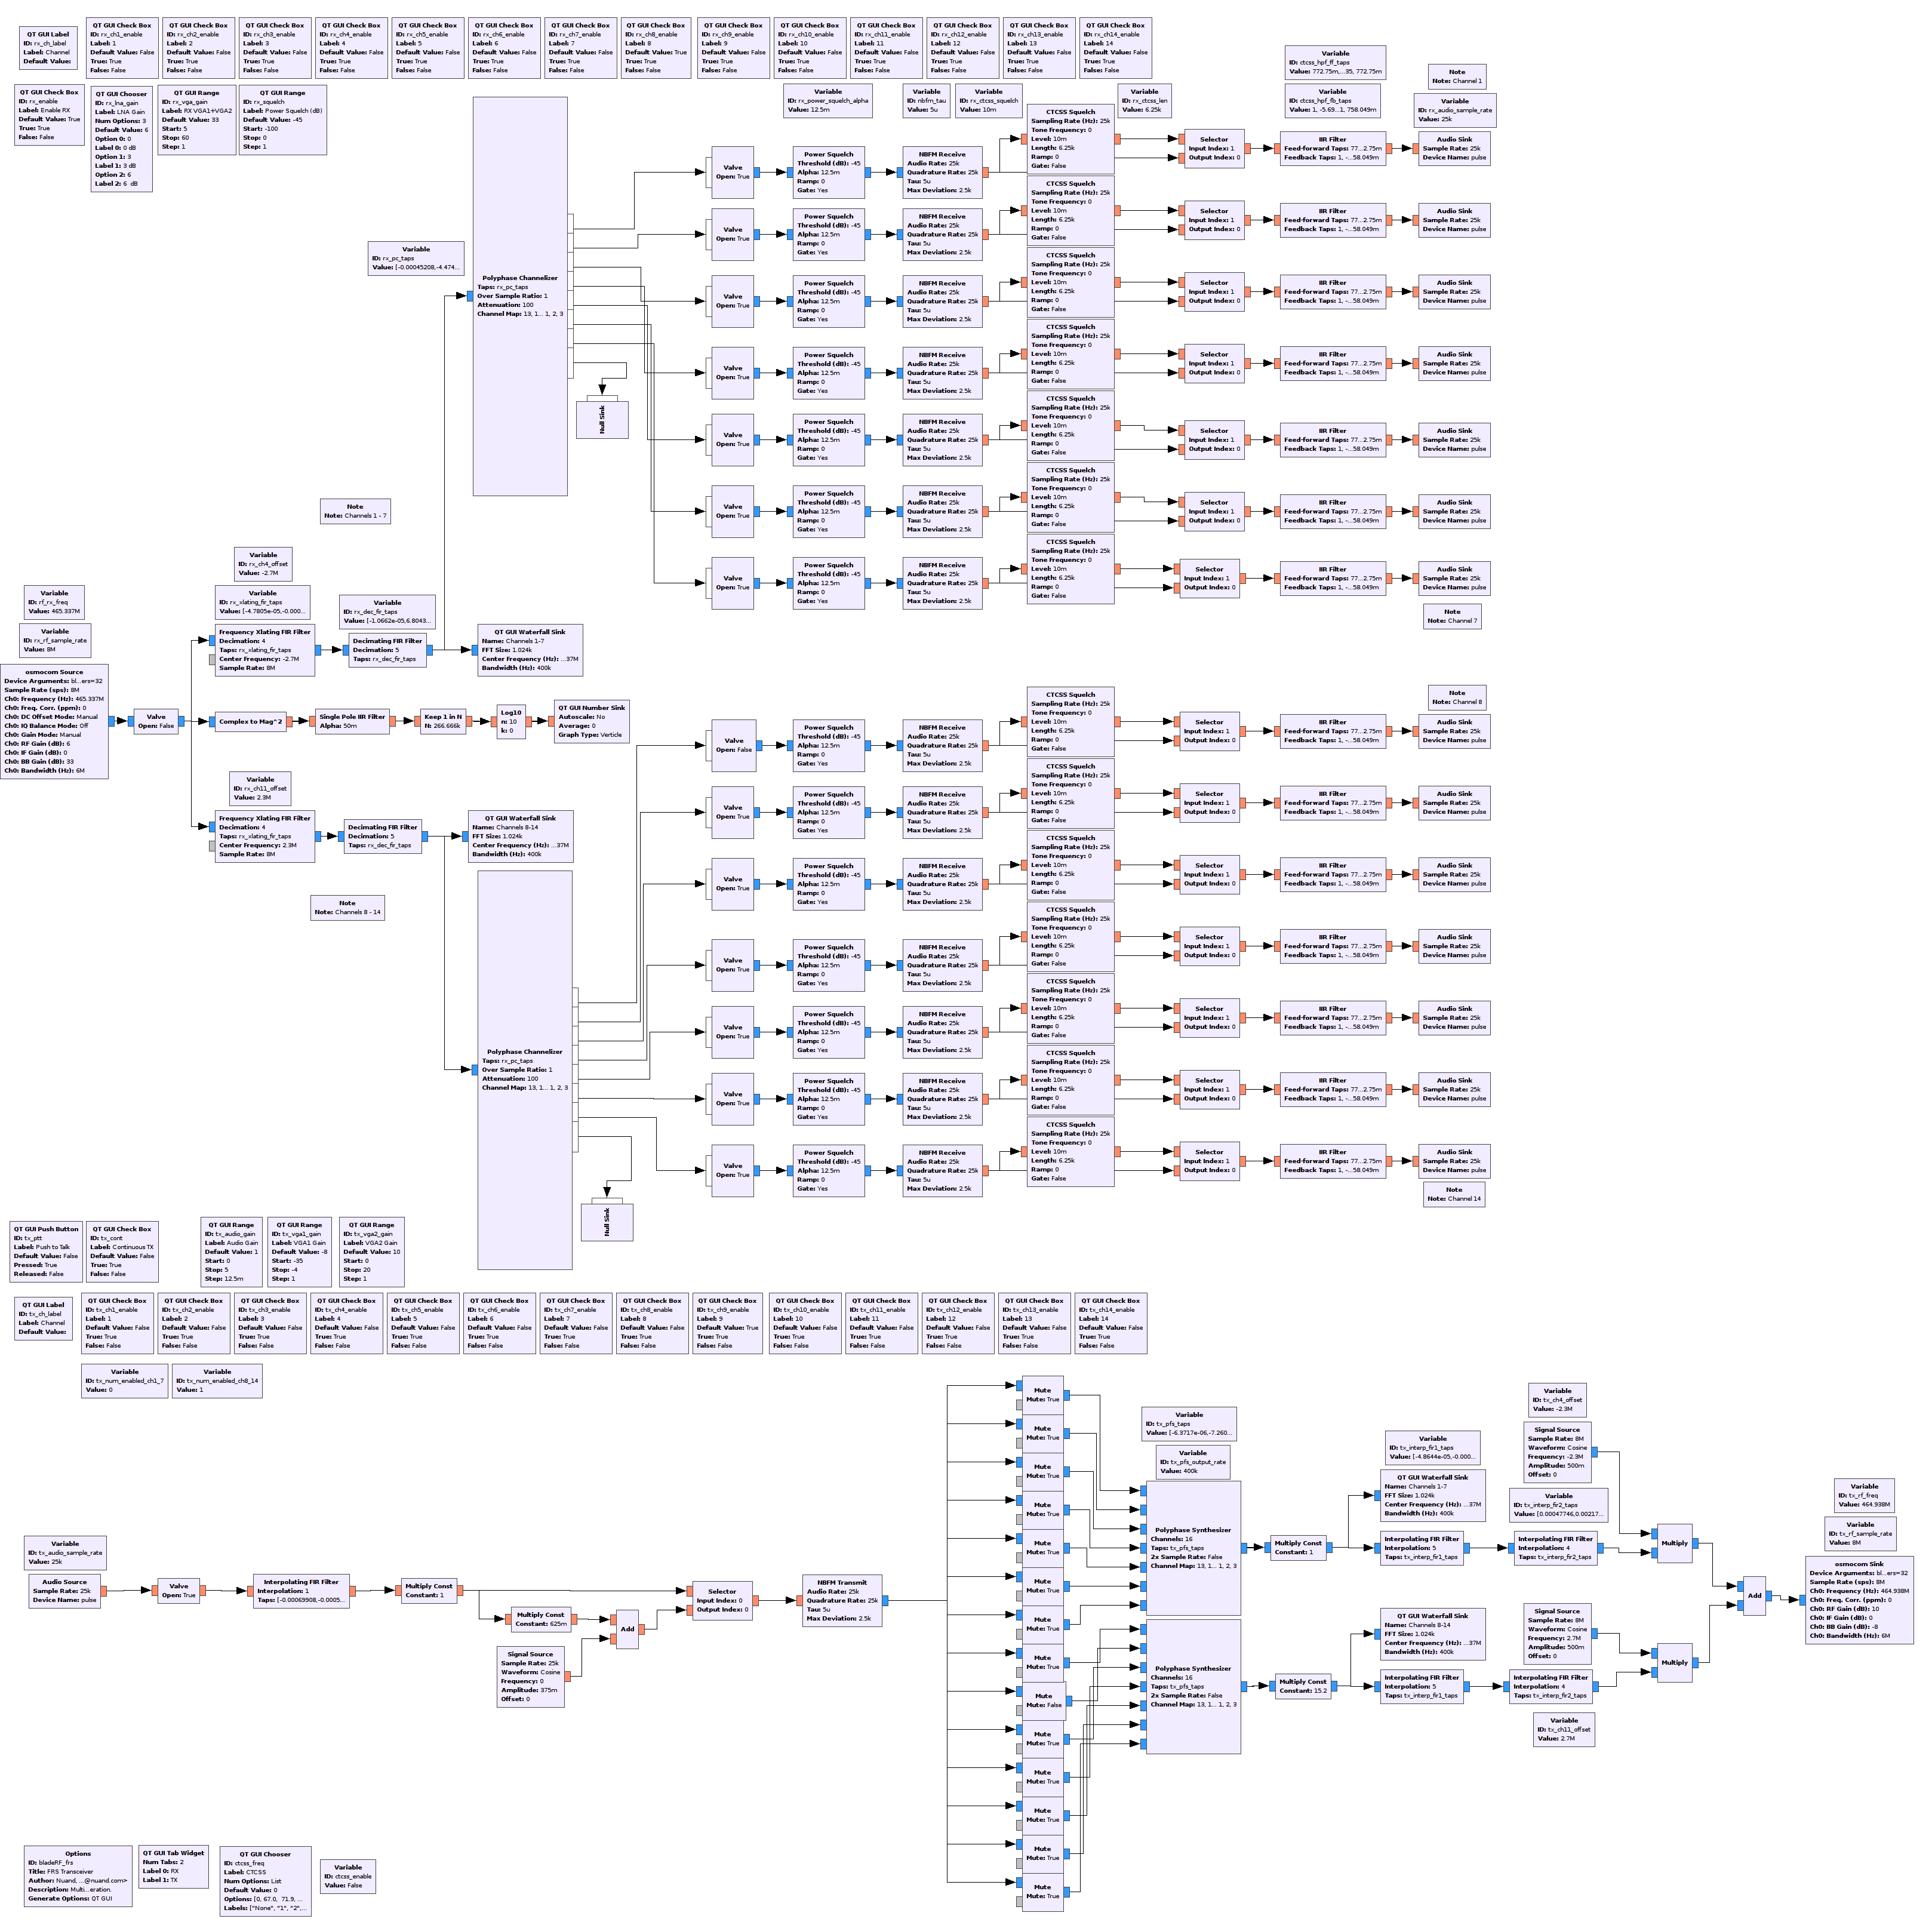
\includegraphics[width=6.5in]{images/frs/bladeRF_frs_grc.png}
  \caption{Full FRS transceiver flowgraph}
\end{figure}

\newpage
\begin{figure}[h!]
  \label{fig:rx_flowgraph}
  \centering
  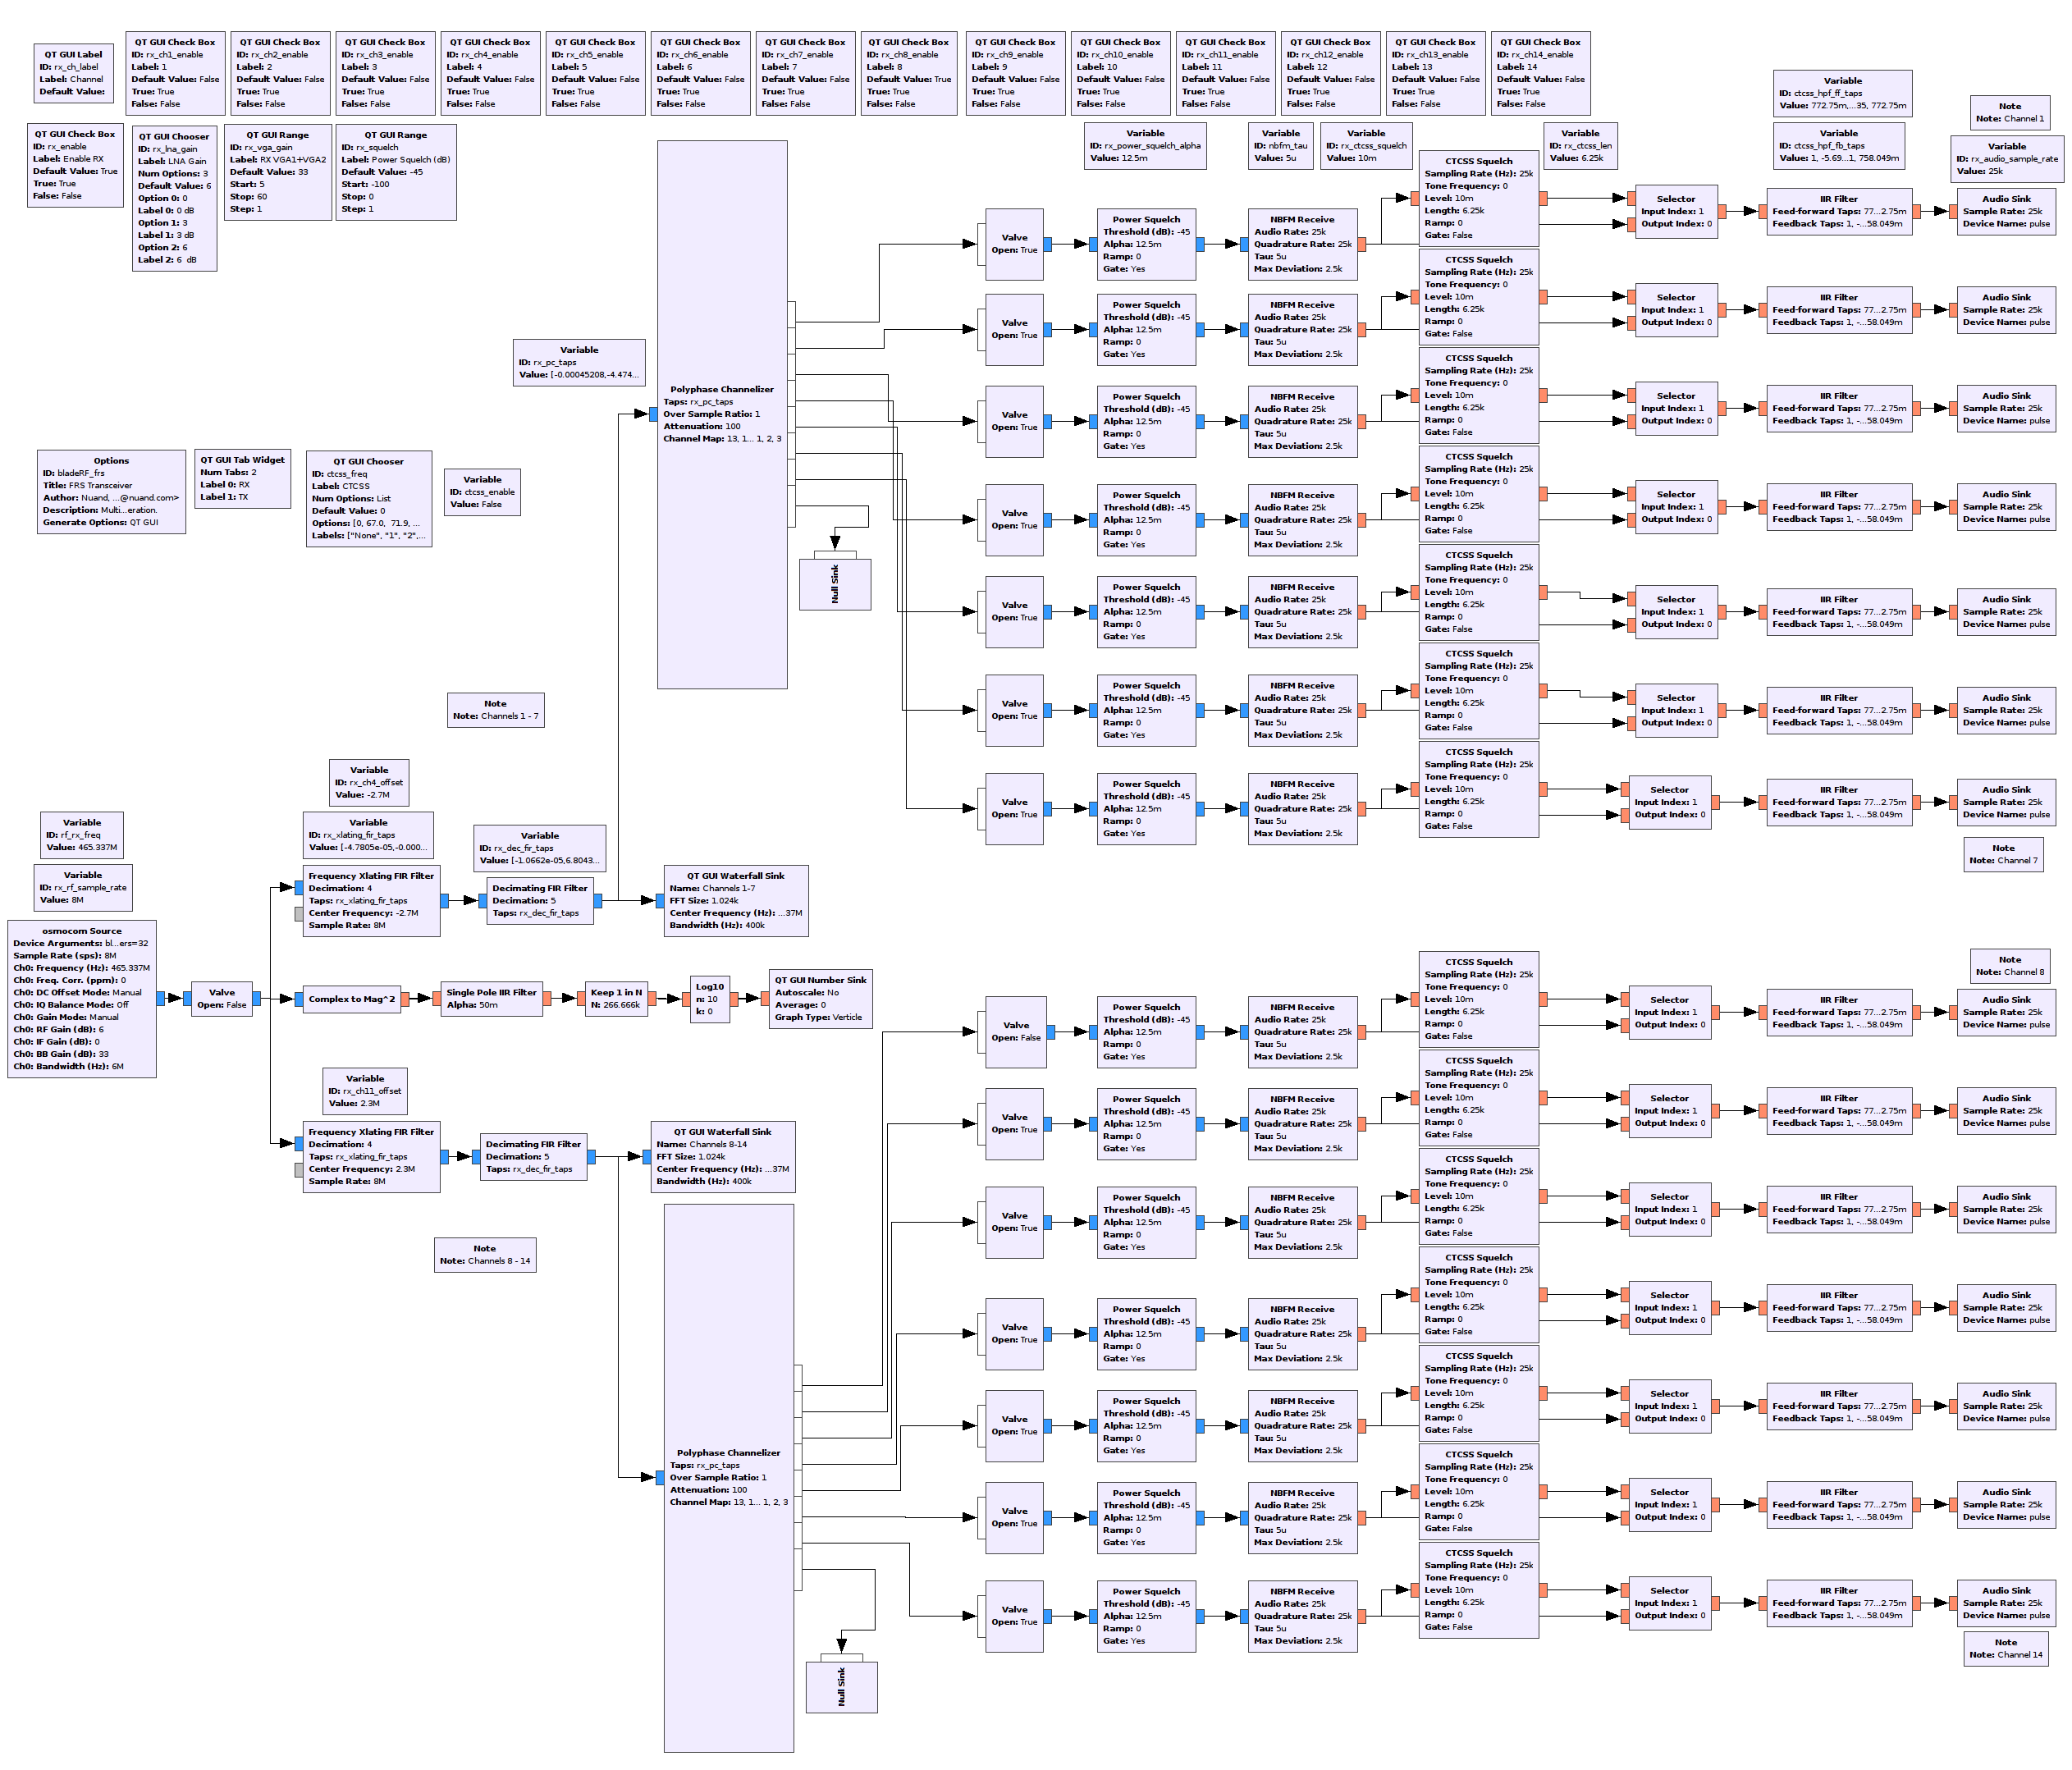
\includegraphics[width=6.5in]{images/frs/bladeRF_frs_rx_grc.png}
  \caption{RX path of FRS transceiver}
\end{figure}

\newpage
\begin{figure}[h!]
  \label{fig:tx_flowgraph}
  \centering
  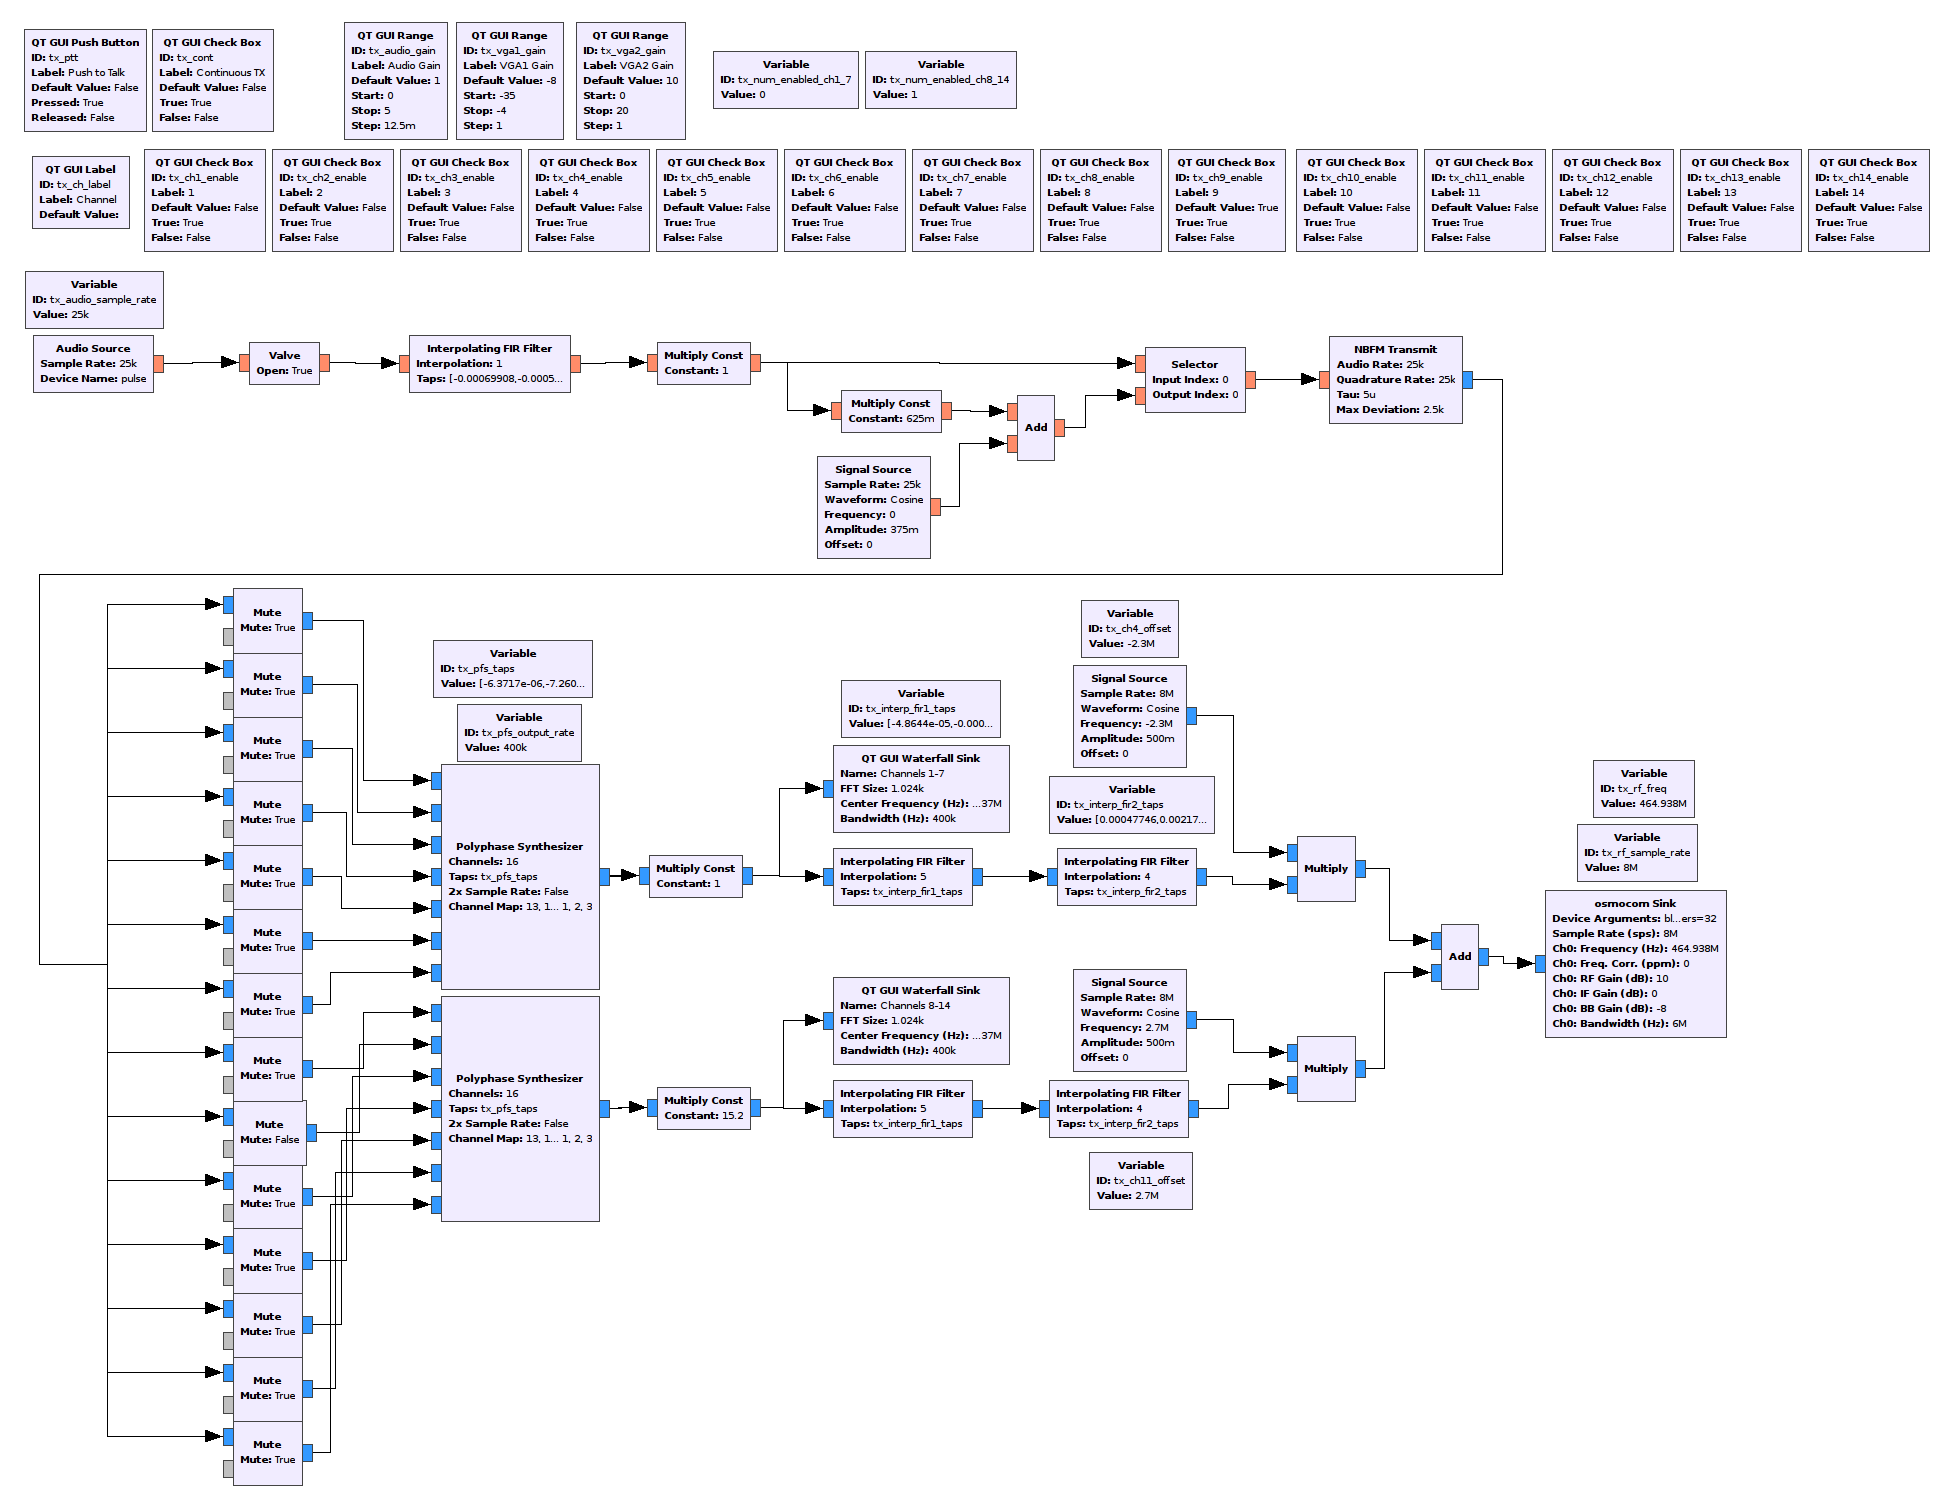
\includegraphics[width=6.5in]{images/frs/bladeRF_frs_tx_grc.png}
  \caption{TX path of FRS transceiver, slightly re-arranged to fit page}
\end{figure}

\newpage
{\footnotesize \bib}
\end{document}
